\chapter {Corpus Study}
\label{Corpus Studies}


The corpus study was conducted to investigate gemination in natural, conversational speech. 
The data was extracted from the Switchboard Corpus (\citealt{Godfrey.1997}), which consists of over 3 million words and comprises North American conversational speech. 
The methodology of the corpus study followed the general methodology described in the previous chapter. However, as the previous chapter was restricted to the description of the general methodology followed in both gemination studies presented in this book, i.e. the corpus and the experimental study,  it is necessary to describe the methodology specific to the corpus study in further detail. This will be done in the first part of this chapter.
 First, I will describe how the corpus data was collected. Then, I will turn to the decomposability rating which was conducted to code the variable \textsc{SemanticTransparencyRating}. After having discussed the validity and reliability of the rating, I will briefly describe the annotation of the variables in the data set. I will then turn to the two different types of analyses conducted.
 On the one hand, the data was analyzed with regard to decomposability, on the other it was analyzed with regard to consonant duration, i.e. gemination. 
First, I will discuss the decomposability analyses and lay out their results. 
Then, I will turn to the durational analyses. Again, I will describe the conducted analyses and discuss results.  At the end of the chapter, I will summarize the results and briefly discuss them with regard to the predictions made in chapter \ref{Theory}. An extensive discussion of the results and their theoretical implications will be conducted in chapter \ref{Conclusion} alongside with the results from the experimental study.\footnote{Earlier versions of sections \ref{sampling corpus},  \ref{Overview of the Variables in the Data Set corpus}, \ref{overview corpus}, \ref{un corpus}, \ref{in corpus}, and \ref{corpus un in} of this chapter have been published in \cite{BenHedia.2017}.} 


\section{Methodology}

\subsection{Sampling}\label{sampling corpus}

In the corpus study four subsets of complex words were investigated. One subset contains \prefix{un}prefixed words, one \prefix{in}prefixed words,
 one \prefix{dis}prefixed words and one \suffix{ly}-suffixed words. The complex words either feature a phonological double consonant at the morphological boundary (e.g. \textit{unnatural}) or a phonological singleton (e.g. \textit{uneven}).
All double consonants in the data set are surrounded by vowels. Singletons in prefixed words are either followed by a vowel or a consonant. Singletons in suffixed words are preceded by either a vowel or a consonant.

To compile the four data sets, I first extracted all words with one of the desired phonological structures from the corpus using the speech corpus management system LaBB-CAT (\citealt{Fromont.2012,Fromont.20032015}).  
I checked all extracted words for their morphological status by using the criteria described in \sectref{theory:in}.
As expected, the number of prefixed words with morphological geminates was quite low. 
For the prefix \prefix{in},
it turned out that the corpus only contained a few /ɪn/-prefixed tokens with two underlying /n/s at the morphological boundary (17 tokens of 5 types). Therefore, I decided to not include the allomorph /ɪn/ in the study, but instead to focus on /ɪm/ for which enough tokens were found. This means that to investigate \prefix{in}, its allomorph /ɪm/ was used (see also sections \ref{scope of gemination} and \ref{corpus data composition} for discussion).

Similarly to \prefix{in} (in its allomorphic form /ɪn/), the number of tokens with a double consonant was quite low for \prefix{un} and \prefix{dis}. For \prefix{un} the corpus contained 22 pertinent tokens, for \prefix{dis} it contained 24 pertinent tokens. In contrast to \prefix{in}, neither \prefix{un} nor \prefix{dis} feature allomorphic variants. In other words, there are no additional tokens with morphological geminates which can be investigated. Therefore, I included all of the available \prefix{un} and \prefix{dis}prefixed tokens with a phonological double, i.e. 22 for \prefix{un} and 24 for \prefix{dis}. 

For \prefix{in} (in its allomorphic form /ɪm/) and \suffix{ly}, the number of tokens with a phonological double was much higher than for \prefix{un} and \prefix{dis}. However, a closer look revealed that a lot of the available tokens were of the same type. Including a lot of tokens of the same type was not desirable for two reasons. 
First, one aim of this study is to investigate word-specific factors. It is therefore crucial to include a high number of different types. 
Second, including a high number of tokens of one type, while only including a low number of tokens of another, might cause serious statistical problems. If the type-token ratio in a data set is very unbalanced, statistical models will be highly influenced by specific types, i.e. by those types which occur frequently in the data set. Including a random effect for type in the model would not provide a solution. This is because the variation found in types which only occur a few times in the data set would be accounted for by the random effect exclusively, i.e. the variation of infrequent types would be explained by inherent differences between types. This would make it impossible to find any other effects. 
It was thus decided to avoid large numbers of tokens of the same type by restricting the number of tokens with a double consonant for \prefix{in} and \suffix{ly} to 90.  


The 90 \prefix{un} and the 90 \suffix{ly}-affixed tokens with a phonological double were semi-randomly selected from the list of all available tokens.  
The semi-random selection included selecting as many different types as possible, and selecting only one token of each type from one pertinent speaker.
Most speakers in the Switchboard Corpus provided us with only one pertinent token, which would have made it impossible to incorporate speaker-specific effects in the statistical analysis. I therefore decided to include only one token of a specific type from one given speaker. 

Note that, while selecting only one token of one type per speaker was possible for \prefix{in} and \suffix{ly}, the small number of items with double consonants in the \prefix{un} and \prefix{dis}subsets prohibited this selection procedure for \prefix{un} and \prefix{dis}. 
In other words, while for \prefix{in} and \suffix{ly}, all tokens of the same type come from different speakers, and all speakers provided only one token per type, for \prefix{un} and \prefix{dis}, two speakers contributed two tokens for one type. 


For all affixes, the selection of words with a singleton at the morphological boundary was executed in a similar way to the selection of \prefix{in} and \suffix{ly}-affixed words with a double consonant, i.e. the items were semi-randomly selected. To keep the data sets as large as possible (to ensure sufficient statistical power), but to also keep the differences in size between the subsets relatively small, the number of singleton tokens in the study was restricted. For the prefixes, 70 tokens were sampled for each of the singleton environments. For \suffix{ly}, 90 tokens were sampled for each environment. 
Hence, I included 70 \prefix{in}prefixed tokens with a single nasal (e.g. \textit{impossible}),  90 \suffix{ly}-suffixed tokens with a single lateral (e.g. \textit{truly, probably}), and 140 \prefix{un} and \prefix{dis}prefixed tokens with a singleton each. For \prefix{un} and \prefix{dis}, 70 of the singletons were followed by a vowel (e.g. \textit{unable}, \textit{disarm}) and 70 were followed by a consonant (e.g. \textit{unfit}, \textit{disgrace}).

After compiling the list of word tokens to be included, I extracted the sound files containing the pertinent tokens from the corpus. All tokens were segmented according to the criteria described in \sectref{Acoustic Analysis}, and afterwards coded for their environment.
Some of the tokens sampled had to be removed after closer inspection of the sound files,  for example because the quality of the recording was insufficient to provide valid segmentation, or because they were pronounced in very unnaturally-sounding ways. The final data sets were of comparable size and contained 158 \prefix{un}prefixed words, 156 \prefix{in}prefixed words (with the allomorph /ɪm/), 128 \prefix{dis}prefixed tokens and 154 \textit{ly-}suffixed words.  The type and token distribution for each environment for each affix is displayed  in \tabref{tbl:distribution of types and tokens in corpus}.


\begin{table}
	\caption{Distribution of types and tokens in corpus study}
	\label{tbl:distribution of types and tokens in corpus}
	
		
		\begin{tabular} {llrr}
				\lsptoprule	
			%\\		
			\textbf{un-}&&&\\
		%	\\
						\midrule   	
			Environment & Example & Number of Types & Number of Tokens\\
			\midrule
			n\#nV&\color{lsMidBlue}\textit{unnatural} & 6 & 23\\ 
			n\#C&\color{lsMidBlue}\textit{untold} & 53 & 68\\ 
			n\#V&\color{lsMidBlue}\textit{uneven} & 42 & 67\\
			\midrule
			Total&  & 101 & 158\\ 
			\midrule
		%	\midrule
			\\
			\textbf{in-}&&&\\
		%	\\
						\midrule   	
			Environment & Example & Number of Types & Number of Tokens\\
			\midrule
			m\#mV&\color{lsMidBlue}\textit{immortal} & 16 & 89\\ 
			m\#C&\color{lsMidBlue}\textit{impossible} & 67 & 67\\ 
			\midrule   
			Total&  & 83 & 156\\ 
			\midrule     	
	%		\midrule
			\\
			\textbf{dis-}&&&\\
		%	\\
									\midrule   	
			Environment & Example & Number of Types & Number of Tokens\\
			\midrule
			s\#sV&\color{lsMidBlue}\textit{dissatisfied} & 9 & 24\\ 
			s\#C&\color{lsMidBlue}\textit{disgrace} & 21 & 45\\ 
			s\#V&\color{lsMidBlue}\textit{disarm} & 34 & 59\\ 
			\midrule   	
			Total&  & 64 & 128\\ 
			\midrule   	
	%		\midrule
			\\
			\textbf{-ly}&&&\\
		%	\\
						\midrule   	
			Environment & Example & Number of Types & Number of Tokens\\
			\midrule
			non-syllabic l\#l &\color{lsMidBlue}\textit{really} & 29  & 33 \\ 
			syllabic 	l\#l &\color{lsMidBlue}\textit{ment(a)lly} & 48 & 48 \\ 
			\#l &\color{lsMidBlue}\textit{possibly} & 73 & 73\\ 
			\midrule   	
			Total&  & 150  & 154\\ 
		%	\midrule   	
			\lspbottomrule                                                                                
		\end{tabular}
		
	
\end{table}







\subsection{The decomposability rating} \label{decomposability rating corpus}

%intro, what was done and what will I say in this para
All types included in the corpus study were rated for their decomposability in terms of semantic transparency. The rating was carried out online using the software LimeSurvey (\citealt{LimeSurveyProjectTeam.2015}). All raters were native speakers of American English. The median rating of each item was coded in the variable  \textsc{SemanticTransparencyRating}. Before the median was computed, the ratings were tested for their reliability and their validity. In this section, I will describe the design of the rating and the analyses conducted to ensure reliability and validity. 

The rating was designed similar to the rating conducted in \cite{Hay.2001}, in which participants were asked to decide which of two derivatives was more complex. As in Hay's task,  participants read an explanation about the make-up of complex words before rating the words' decomposability.  The participants were informed that some words consist of more than one meaningful unit and were given examples. 
They were then asked to rate on a scale from 1 to 4 how easy it is to decompose the words into two meaningful units. The participants were explicitly told which units to look for, e.g.\textit{ in} and rest of the word for the rating of \prefix{in}prefixed words, and \textit{un} and rest of the word for \prefix{un}prefixed words. The participants were given the opportunity to  indicate if they did not know a word. 
Some biographical information about the participants, such as their language background, their profession, and their knowledge about linguistics, was recorded in order to test whether any of these factors influenced the rating.\footnote{The questionnaire the participants of the rating studies filled out, and the instructions they were given can be found in \hyperref[Appendix A: Decomposability Rating]{appendix A}. } 

Four ratings were conducted, two ratings included \prefix{un} and \prefix{in}prefixed words, one \prefix{dis} prefixed words and one \suffix{ly}-affixed words. In addition to the complex words included in the corpus study, the ratings also included simplex words which featured the same orthographic strings as the affixed words, e.g. \textit{{un}cle} and \textit{fami{ly}}. They were included to test whether the raters understood the task correctly. Simplex words should be rated as being very difficult to decompose. 

All in all 133 native speakers of American English between the ages of 14 and 62 rated 450 items. 
After the ratings were conducted, I analyzed the data in order to test the validity and the reliability of the rating. As a first step, I checked the distribution of ratings for each participant. Participants who did not vary in their rating, i.e. who rated all the items the same, and participants who rated the simplex items as very decomposable were excluded. It can be assumed that they either did not understand the task correctly, or did not fulfill the task thoroughly. Their ratings were not valid.
To further check the ratings' reliability, I computed three consistency estimates of inter-rater reliability, the intraclass correlation coefficient (ICC, \citealt{Bartko.1966}), item-total correlations and Cronbach's $\alpha$ (\citealt{Cronbach.1951}). All three measures can be used to test whether the subjects rated the items with internal consistency (see also \citealt[38 ff.]{Stemler.2008} for discussion). 

The intraclass correlation coefficient (ICC) assesses the agreement rate of multiple responses across different stimuli, i.e. it assesses the agreement in the ratings of all raters across all items. Two different ICCs were computed, ICC 2 and ICC 3. While ICC 2 takes differences in the average ratings of the participants into account, ICC 3 does not. For example, if rater 1 rated item A with 1 and item B with 2, while rater 2 rated item A with 2 and item B with 3, the ICC 2 would show perfect agreement between the two raters (an ICC 2 of 1). Taking the difference in the intercept into account, rater 1 and rater 2 agreed perfectly by rating item B with one value more than item A. The absolute agreement of the ratings would, however, not be perfect because the two raters did not rate both items with the same values. This degree of absolute agreement is shown by ICC 3, which would be below 1 in the example.

The second measure of consistency are item-total correlations. This measure computes the correlation between the ratings of one participant and the ratings of all other participants across all items. This means that one value for each participant is computed. This measure can be used to detect participants which differed to a high degree from the other participants in their rating. After inspecting the distribution of item-total correlations across speakers, I excluded all participants whose item-total correlation was clearly lower than the other participants' correlations. This resulted in excluding all participants who featured an item-total correlation below 0.6. 

The third measure of inter-rater reliability is Cronbach's $\alpha$, which is a reliability coefficient often used to measure internal consistency. Cronbach's $\alpha$ displays the average inter-correlation among raters across items. Its value is between 0 and 1 with 1 indicating excellent internal consistency and 0 unacceptable internal consistency. 
I computed all measures using the R package \texttt{psych} (\citealt{Revelle.2017}).




After excluding invalid ratings, based on the inspection of the ratings' distributions and the analysis of inter-rater reliability, the ratings proved to be valid and reliable. This is indicated by the consistency estimates which are summarized in \tabref{tbl:Overview consistency estimates for all ratings in corpus studys} for all ratings. For the item-total correlations, the minimum, the maximum, the mean and the median correlations for each rating are displayed. The table also shows the final number of raters for each rating, i.e. the number of raters after the exclusion of invalid raters. All in all, 23 raters were excluded.


\begin{table*}
	\caption{Overview consistency estimates for all ratings in corpus study}
	\label{tbl:Overview consistency estimates for all ratings in corpus studys}
	
		\resizebox{\textwidth}{!}{%
			\begin{tabular} {lrrrrrrrr}
			
			
			\lsptoprule
				&number &			  &  & &&  &  & \\
				&of raters& Cronbach's \textbf{$\alpha$ }&ICC1 & ICC 2& \multicolumn{4}{r}{item-total correlation}\\
				\midrule
				&  &&&&Min & Max& Mean& Median  \\
				\midrule
				\midrule
				Rating 1:		& &&  & &&&&\\ 
				\prefix{un} and 
				\prefix{in}&26&0.99& 0.75 &0.77 &   0.69& 0.95& 0.88& 0.91 \\  
				
				
				\midrule
				
				
				Rating 2:& &&  & &&&&\\ 
				\prefix{un} and \prefix{in}&32 &0.99 &0. 69 & 0.72 &0.69&  0.94& 0.85& 0.87 \\   			
				
				\midrule
				
				Rating 3:& &&  & &&&&\\ 
				\prefix{dis}& 32& 0.98&  0.62 &0.66 & 0.63 &0.91& 0.83 &0.81\\   			
				\midrule
				
				
				Rating 4: & &&  & &&&&\\ 
				\suffix{ly}& 20 &0.98 & 0.72 & 0.72 &0 .62 &1.0 &0.93 &0.99   \\  			
				%			\midrule
				\lspbottomrule                                                                                
		\end{tabular}
		}
	
\end{table*}



After the reliability of the ratings was ensured, I checked for possible effects of age, sex and linguistic background (including knowledge of Latin and linguistics) on the rating by conducting regression models. The dependent variable of these models was the rating. Fixed factors included age, sex, linguistic background and knowledge of Latin. The participant was included as a random effect. The analyses showed that neither age, nor sex,  nor the linguistic background or knowledge of Latin had a significant effect on the rating.

I computed the median rating for each type and coded it in the variable \textsc{Seman-ticTransparencyRating}. I chose to code the median in the variable, i.e. not the mean, to avoid the influence of a few extreme ratings. 






\subsection{Annotation} \label{Overview of the Variables in the Data Set corpus}

After extracting and phonetically annotating the words included in the corpus study, they were annotated with regard to factors possibly influencing consonant duration. These factors were described in detail in \sectref{General method annotation}. Because of differences between corpus and experimental data, not all of the discussed variables were included in both studies. For the corpus study, the five variables \textsc{GlobalSpeechRate}, \textsc{TypeOfL}, \textsc{Accentuation}, \textsc{PrePause} and \textsc{PostPause} were not coded (see variable descriptions in \sectref{General method annotation} for a discussion on why these variables were not included). 
All other variables described in \sectref{General method annotation} were included in the study. 
Overviews of all variables initially included in the models predicting absolute consonant duration are given in tables \ref{tab: summary dep variables un-model} -- \ref{tbl: corpus summary varables ly} in \hyperref[App B: Summaries of variables in initial models of corpus study]{appendix B}. 




\section{Decomposability} \label{corpus dec}

Analyzing decomposability had two aims. The first aim was to test the suitability of the decomposability measures used in this study. This was done by investigating the relation between the different decomposability measures.  
The second aim was to test the validity of the segmentability hierarchies proposed in \sectref{comparison affixes}.  This is important with regard to the theoretical predictions proposed in chapter \ref{Theory}. To test whether the hierarchies are validated by the data, the segmentability of the five affixes was compared.




\subsection{The relation between decomposability measures} \label{The Relation between Decomposability Measures} 
 


As discussed thoroughly in \sectref{decomposability}, we find different operationalizations of decomposability in the literature. It is yet unclear whether all of them are well-suited measures of the concept. In this study five variables are used as potential measures of decomposability: \textsc{SemanticTransparency}, \textsc{SemanticTransparen-cyRating}, \textsc{TypeOfBase}, log\textsc{Re-lativeFrequency} and \textsc{LSAScore}.
To test whether all of these variables tap into the same phenomenon, i.e. decomposability, it is necessary to investigate their relation to each other. If they are all measures of the same underlying property, they are expected to be highly correlated. To test the relation between the variables, hierarchical cluster analyses were conducted. 

Hierarchical cluster analyses are usually used to find patterns and groups with similar characteristics in a data  set (see, for example, \citealt[chapter 5.1.5]{Baayen.2008}, \citealt[chapter 8.1]{Zumel.2014}). They can also successfully be applied to investigate the similarity between different variables, and are thus well suited to provide insights into the relation between the five decomposability variables (see \citealt[200 f.]{Baayen.2008}). 
The type of cluster analysis applied here first computes Spearman's rank correlations between all included variables, then squares them, and then puts them into a correlation matrix. This matrix hence includes pairwise comparisons of all decomposability variables. The use of squared figures is motivated by the need to avoid negative values.
Since correlations can only be calculated for numerical variables,  categorical variables have to be recoded into numerical variables in order to be included into the analysis. 
Therefore, the categorical variable \textsc{SemanticTransparency}  was recoded into the numerical variable \textsc{numSemanticTransparency}, and the categorical variable \textsc{TypeOfBase} was recoded into the numerical variable \textsc{numTypeOfBase}.  The variable \textsc{numSemanticTransparency} featured  the two levels 0 (=~opaque) and 1 (=~transparent), the variable \textsc{numTypeOfBase} the levels 0 (=~bound root) and 1 (=~word as base). After the correlation matrix was created,  a dendrogram in which the correlations are displayed was generated. Variables which cluster together in the dendrogram are more similar, i.e. have a higher correlation, than variables which are more distant in the dendrogram. 

I conducted five cluster analyses, one for each subset and one for the whole data set. 
I decided to not only conduct one analysis looking at the whole data set, but to also investigate the relation between the variables in each of the four subsets, to check for possible differences between subsets. The affixes might deviate in their segmentability (as will be discussed in further detail in \sectref{The decomposability of the four affixes: a comparison}), and these differences between affixes might be mirrored in the relation between the different decomposability variables in the subsets, i.e. the correlations might deviate between subsets.

All analyses were based on types, not on tokens. Types were chosen to avoid that the decomposability features of one very frequent type in the data set affect the results for the whole data set. In other words, to avoid that the correlations between the variables were influenced by the relation between them in one specific type, each type was only included once in the analyses. 
All in all, 396 types were analyzed. However, for the correlations with the variable \textsc{LSAScore}, not all types could be considered. This is due to the fact that, as explained in \sectref{variables of interest}, a similarity score can be computed only for derivatives with words as bases, and thus only derivatives with words as bases were coded for \textsc{LSAScore}. It follows that the correlations between the variable \textsc{LSAScore} and all other variables only considered those items for which the score was available (303 types). For all other correlations all 396 types were taken into consideration. 
All cluster analyses were generated in R using the \texttt{Hmisc package} (\citealt{Harrell.2017}).

The first cluster analysis conducted investigated all types of the corpus study, i.e. derivatives with all five affixes. The correlation matrix created in the analysis is shown in \tabref{tab: Correlation matrix for all decomposability measures in corpus study}. The table shows that the highest correlations are between the variables \textsc{numSemanticTransparency}, \textsc{SemanticTransparencyRating} and \textsc{numTypeOfBase}. The correlations between log\textsc{RelativeFrequency} and \textsc{LSAScore} and all other variables are much lower. 



 
 \begin{table*}

	\caption{Correlation matrix for decomposability measures in corpus study}
	\label{tab: Correlation matrix for all decomposability measures in corpus study}
	
	\resizebox{\textwidth}{!}{%
\begin{tabular}{lrrrrr}
\lsptoprule
 &\textsc{numSemantic-}  & log\textsc{Relative-} &  \textsc{SemanticTrans-}      &\textsc{numType-} &\textsc{}\\
  &\textsc{Transparency}  & \textsc{Frequency} &  \textsc{parencyRating}      &\textsc{OfBase} &\textsc{LSAScore}\\
 
 \midrule

 \textsc{numSem.Transp.}                 &     1.00        &           &   &  &   \\
 log\textsc{Rel.Freq. }                &     0.09        &          1.00    &&   &   \\
 \textsc{Sem.Transp.Rating}                                    &    0.70             &     0.10    &1.00   & & \\
 \textsc{numTypeOfBase}                   &            0.65      &           0.08 &   0.70  & 1.00  &    \\
 \textsc{LSAScore}                             &       0.11             &     0.03  &  0.08   & 0.05     & 1.00\\
 \lspbottomrule                                                                                
		\end{tabular}
}

 \end{table*}
 
 
 


 

 
  \figref{fig:cluster corpus all affixes} displays the relation between the variables in a dendrogram. On the y-axis the squared Spearman correlation score between the variables is displayed. 
  The figure shows three splits which structure the variables into four clusters. The lower the splits in the figure, the higher are the correlations between the variables of the pertinent clusters.
      The first split separates the  variable \textsc{LSA-Score} from all other variables. \textsc{LSAScore} thus forms its own cluster, which indicates the dissimilarity of this variable to the other four decomposability variables. The second split separates the variable log\textsc{RelativeFrequency} from \textsc{numSemanticTransparency}, \textsc{SemanticTransparencyRating} and \textsc{numTypeOfBase}. This shows that log\textsc{RelativeFrequency} is also rather dissimilar from the other three decomposability variables. 
      That log\textsc{RelativeFrequency} and \textsc{LSAScore} are different from the other three decomposability variables is also shown by the high position of the first two splits in the figure.
      
      
     \begin{figure*}
    	
    	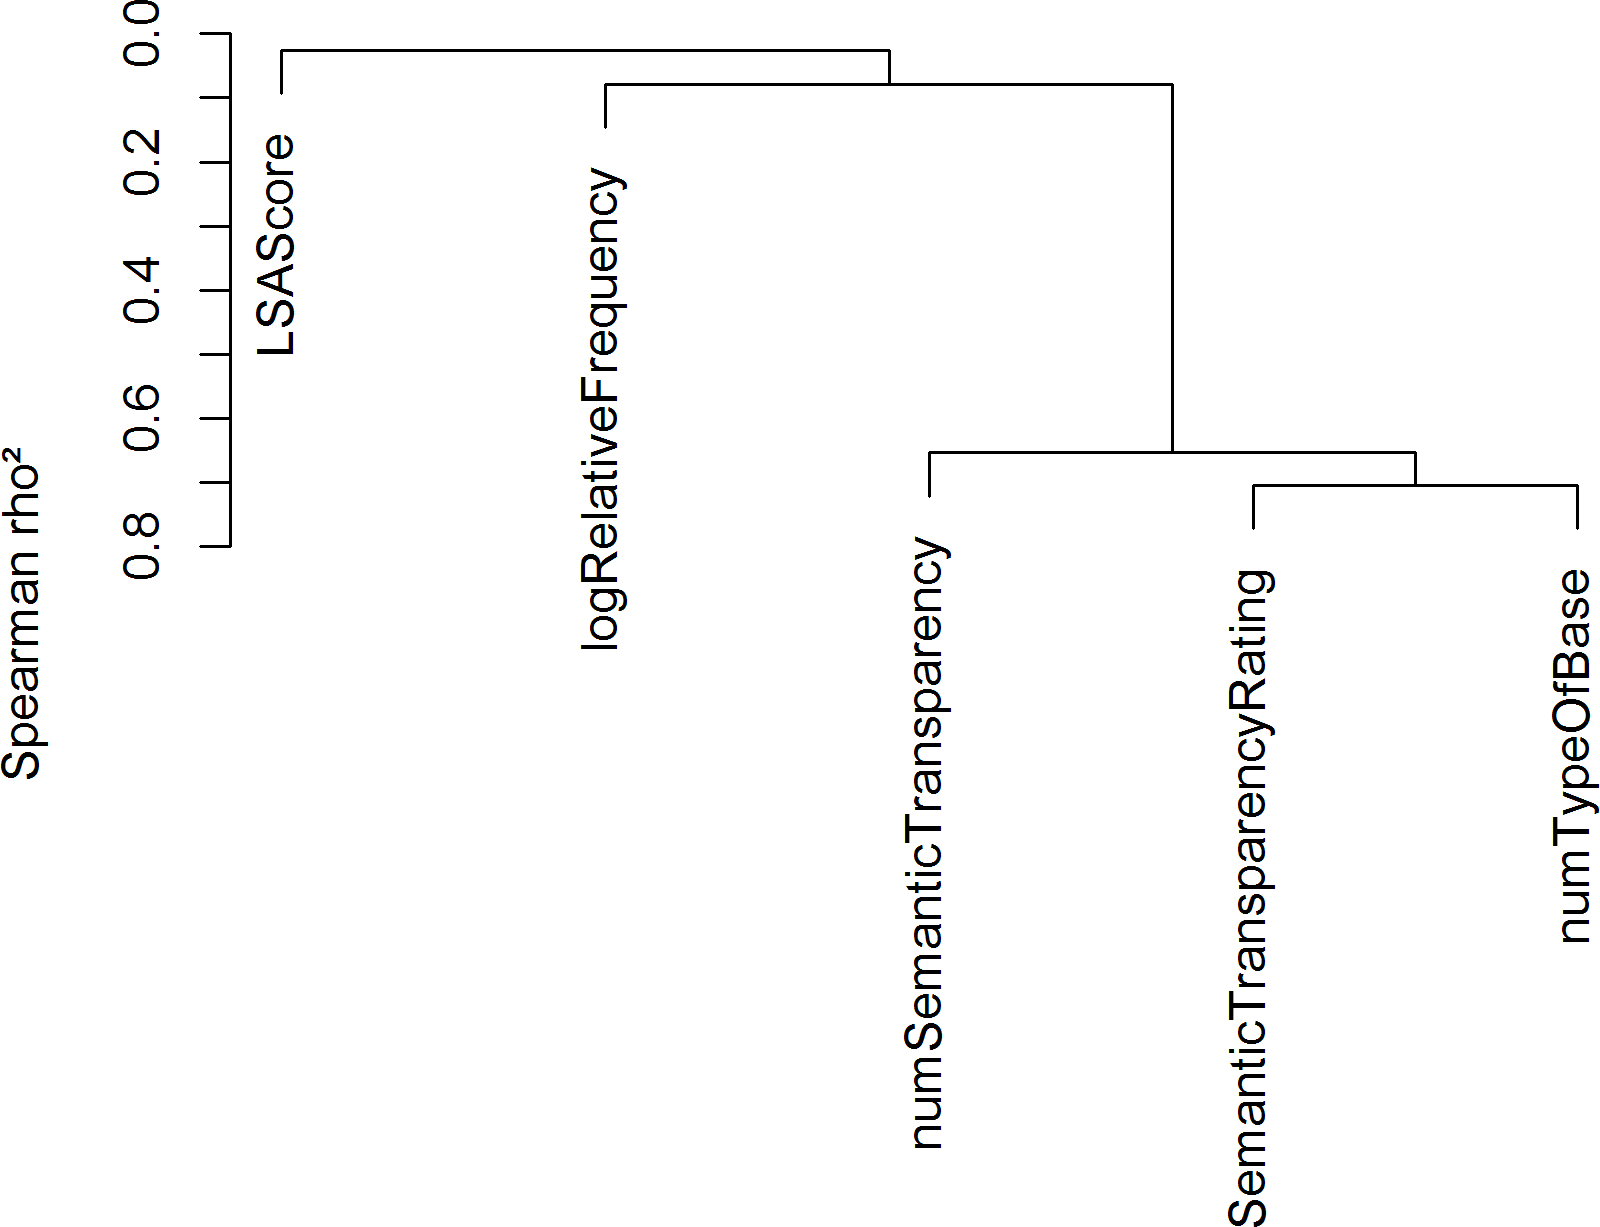
\includegraphics[scale=0.5]{images/Corpus/clusterAnalysisDecomposabilityCorpusAllTypes.png}
    	\caption{ Dendrogram of the five decomposability measures for all types in the corpus study}
    	\label{fig:cluster corpus all affixes}
    \end{figure*}
      
      
  The third split is the one splitting \textsc{numSemanticTransparency} from \textsc{Seman-ticTransparencyRating} and \textsc{numTypeOfBase}. This split is displayed in the lower part of the figure, which indicates that even though  \textsc{SemanticTrans-parencyRating} and \textsc{numTypeOfBase} are more similar to each other than they are to \textsc{numSemanticTransparency}, all three variables correlate to a high degree and are very similar.
  
 
 Let us now turn to the analyses of the individual affixes.
 It turned out that fitting a cluster analysis was only reasonable for the prefixes \prefix{in} and \prefix{dis}, i.e. it was not reasonable to conduct cluster analyses for \prefix{un} and \suffix{ly}. 
 This is due to the distribution of the decomposability variables in the \prefix{un} and the \suffix{ly}-data sets. Three of the five decomposability variables do not show enough variability to be investigated. All of the \prefix{un} and \textit{ly-}affixed words are semantically transparent, and only a few feature a bound root. Furthermore, all \prefix{un}prefixed, and the majority of \suffix{ly}-suffixed words were rated as very decomposable. Because of this lack of variability in the variables \textsc{SemanticTransparency}, \textsc{SemanticTransparencyRating} and \textsc{TypeOfBase}, only the correlation between log\textsc{RelativeFrequency} and \textsc{LSAScore} was investigated for \prefix{un} and \suffix{ly}.
 The squared Spearman correlation score is below 0.05 for all correlations tested. This means there is no indication that the two variables log\textsc{RelativeFrequency} and \textsc{LSAScore} can be used as the operationalization of the same concept.
 
 
 
 
 
 For \prefix{in} and \prefix{dis}, all variables showed enough variation to conduct cluster analyses. The results of the analyses for the two prefixes are displayed in the dendrograms in \figref{fig:cluster corpus dis and in}. 
 For both prefixes, the variables \textsc{numSemanticTransparency}, \textsc{SemanticTransparency-Rating} and \textsc{numTypeOfBase} cluster together in the lower part of the figure. This means that the correlations between the three variables are quite high. \textsc{LSAScore} and log\textsc{RelativeFrequency}, on the other hand, do not correlate to a high degree with any other variable. This resembles the results of the first cluster analysis.

\begin{figure*}  
	
	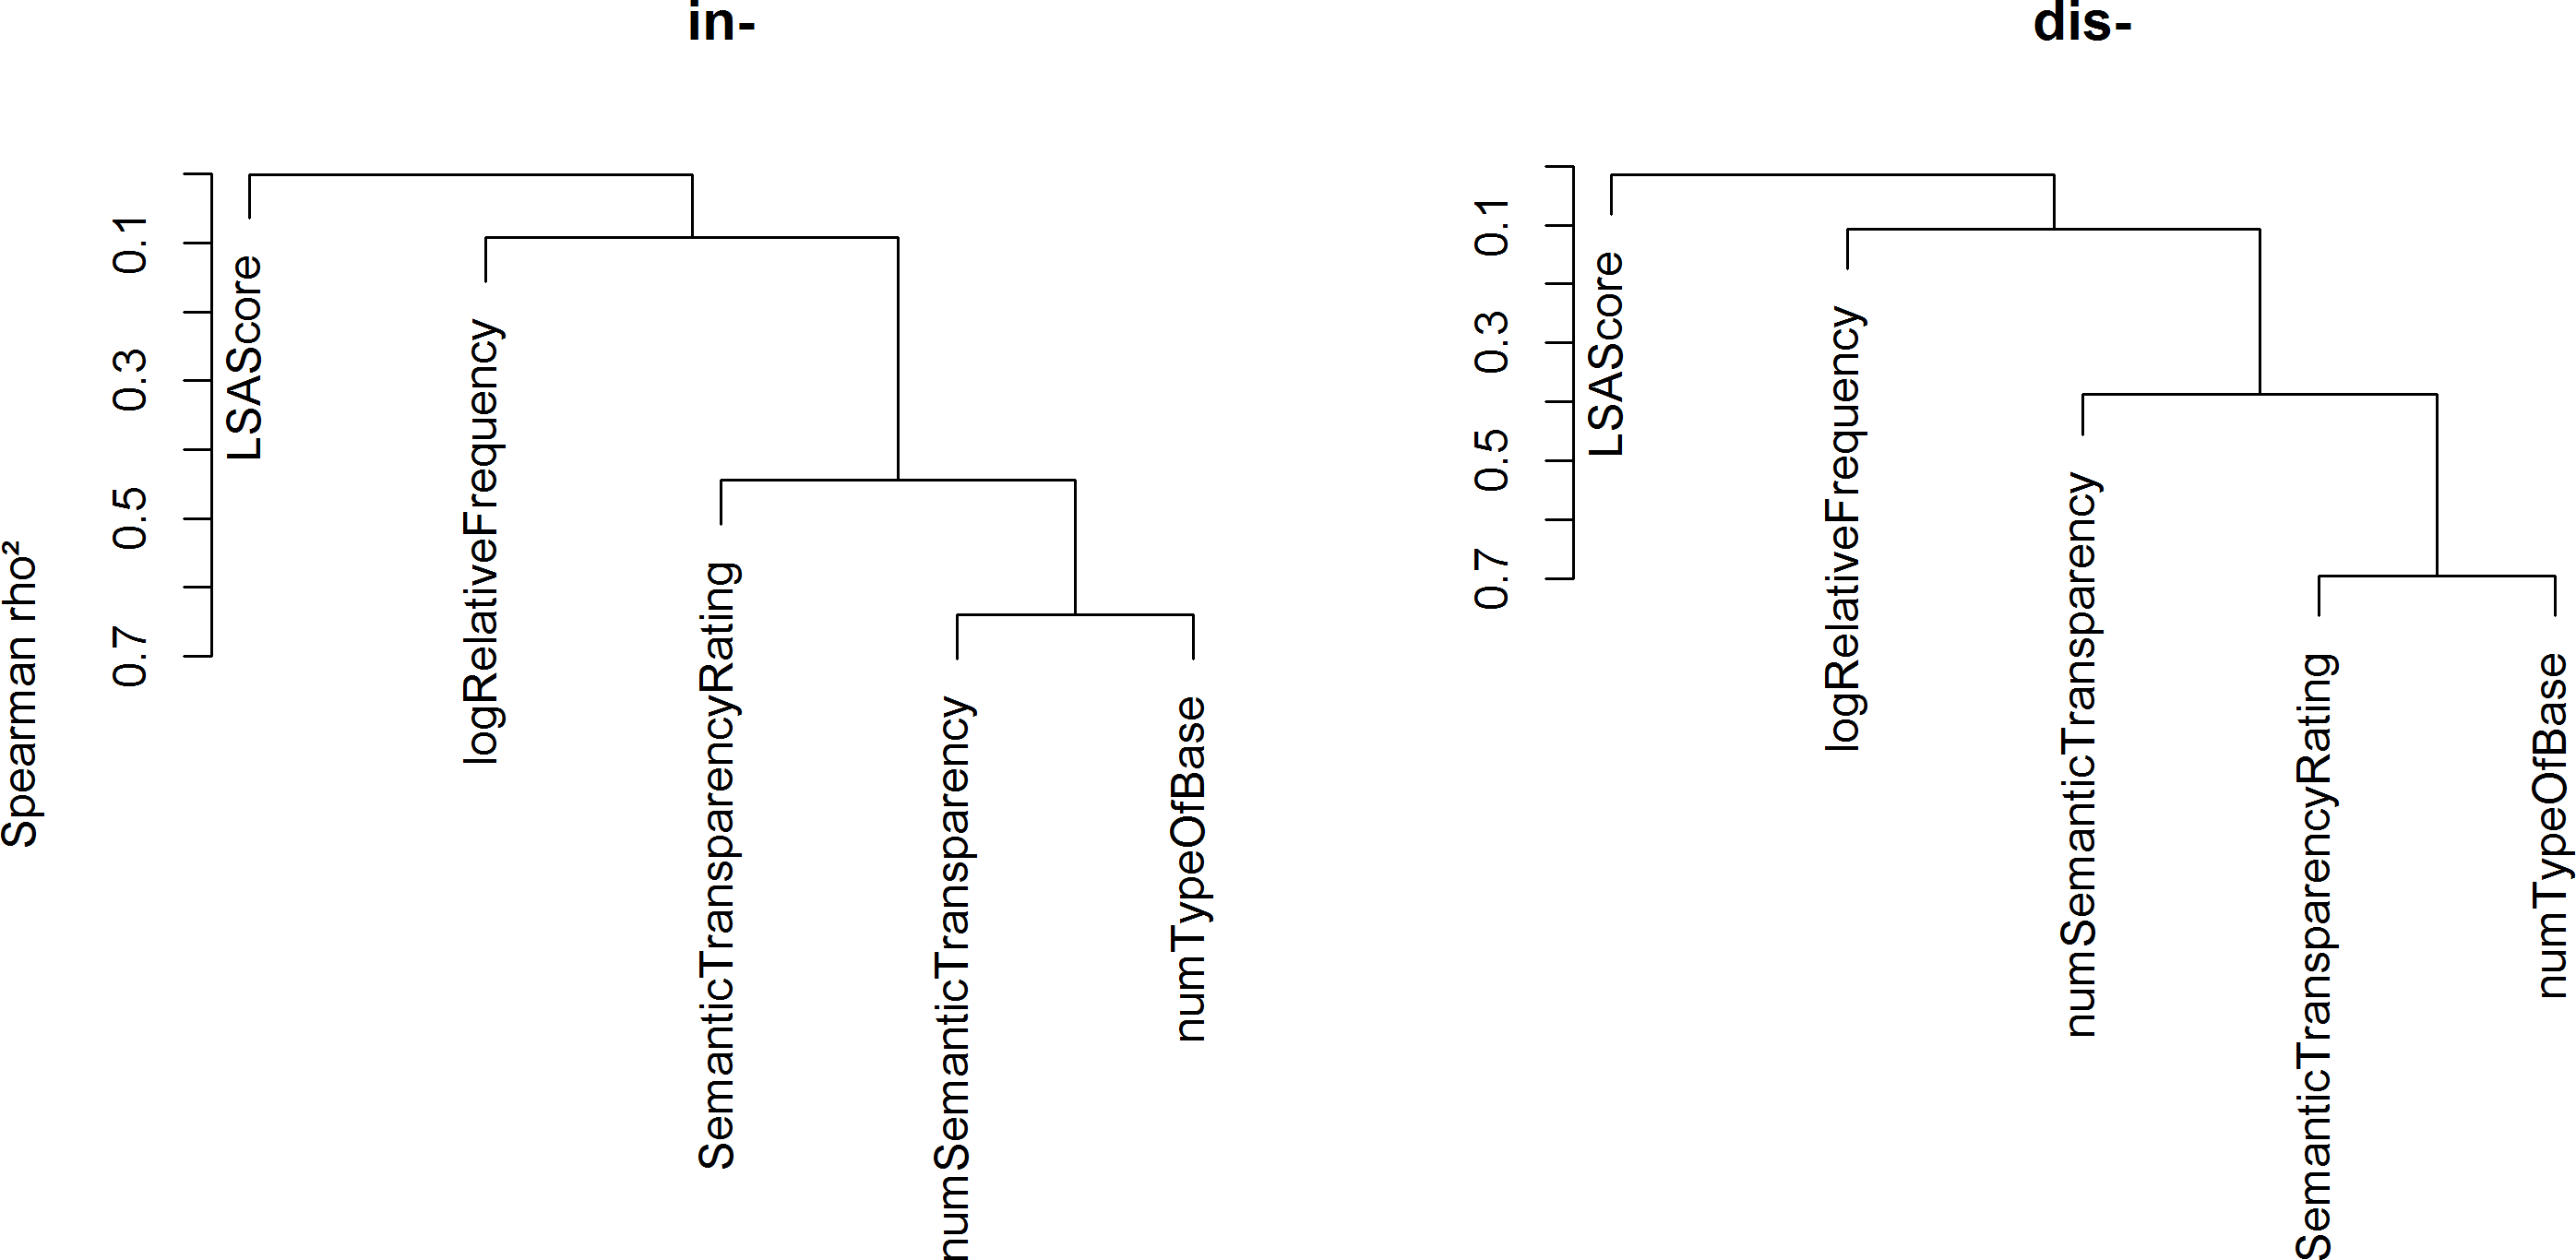
\includegraphics[scale=0.5]{images/Corpus/clusterAnalysisDecomposabilityCorpusDisAndIn.png}
	\caption{ Dendrogram of the five decomposability measures for \prefix{in} and \prefix{dis}prefixed words in the corpus study}
	\label{fig:cluster corpus dis and in}
\end{figure*}



To sum up, the cluster analyses have revealed that the three variables \textsc{Semantic-Transparency}, \textsc{SemanticTransparencyRating} and \textsc{TypeOfBase} are highly correlated. The two variables log\textsc{RelativeFrequency} and \textsc{LSAScore}, in contrast, barely correlate with the other decomposability variables.
These outcomes can be interpreted in the following way: while the three variables  \textsc{SemanticTransparency}, \textsc{SemanticTransparencyRating} and \textsc{TypeOfBase} can certainly be used as measures of the same concept, this cannot be stated for the two variables log\textsc{RelativeFrequency} and \textsc{LSAScore}. In other words,  while possible effects of \textsc{SemanticTransparency}, \textsc{SemanticTransparencyRating} and \textsc{TypeOfBase} on duration are probably caused by the same underlying property, any effects of log\textsc{RelativeFrequency} and \textsc{LSAScore} can be regarded as independent.


The result that only three of the five investigated variables are measuring the same underlying property, i.e. that two measures are independent, raises the question of which variable, or which set of variables, is the right measure of decomposability.
The answer to this question is not trivial and depends on one's definition of the concept \newterm{decomposability}. As thoroughly discussed in \sectref{decomposability}, decomposability is not explicitly defined in the literature and different operationalizations are used. In other words, decomposability is not one uniform theoretical concept and cannot be treated as such. Different operationalizations call for different definitions of the concept. 
The analyses conducted in this section indicate that the decomposability measures used in this study form operationalizations of three different types of decomposability. The first type is operationalized by \textsc{SemanticTransparency}, \textsc{TypeOfBase} and \textsc{SemanticTransparencyRating}, the second is operationalized by log\textsc{RelativeFrequency}, and the third is operationalized by \textsc{LSAScore}.
The answer to the question of which variable measures decomposability is thus that all five variables are measures of decomposability but that they do not measure the same type of decomposability. 

 

\subsection{The segmentability of the affixes: A Comparison}
\label{The decomposability of the four affixes: a comparison}

Two of the theoretical predictions about gemination, i.e. the affix-specific morphological segmentability prediction and the affix-specific morphological informativeness prediction (cf. \sectref{decomposability}), are based on the lexical segmentability hierarchies proposed in \sectref{comparison affixes}. To ensure the validity of these predictions, it is necessary to ensure the validity of the proposed segmentability hierarchies (see \figref{fig:Segmentability hierarchies of  affixes repetition 2} for a repetition of the hierarchies). 
The Semantic Segmentability Hierarchy is mainly based on a qualitative analysis of the affixes' semantics (see discussion on semantics of the affixes in \sectref{comparison affixes}). Testing its validity by a quantitative analysis, such as the one applied here, is therefore quite challenging.
 The validity of the Non-Semantic Segmentability Hierarchy can, however, well be tested by checking whether the hierarchy is mirrored in the distribution of the decomposability measures in this data set.
 
 



\begin{figure*}
		
	
\begin{tabularx}{\linewidth}{lll}
	
	& \textbf{Segmentability}&	\textbf{Additional 	}  		  \\
	
	&	\textbf{hierarchy	}	&		\textbf{assumption }  	  \\		
	\midrule\\
	
	\textbf{Semantic} & \prefix{un} > \{\prefix{dis}, \prefix{in}\textsubscript{\textsc{Neg}}\}>  \prefix{in}\textsubscript{\textsc{Loc}} > \suffix{ly}& lexical meaning over pro-	 		  \\	
	\textbf{Hierarchy}	& & ductivity, transparency and 	 		  \\	
	& & type of base			 		  \\	
	\\
	\textbf{Non-Semantic}	&  	\prefix{un} > \suffix{ly} > \{\prefix{dis}, \prefix{in}\textsubscript{\textsc{Neg}}\}>  \prefix{in}\textsubscript{\textsc{Loc}}&		 productivity, transparency			   \\	
	\textbf{Hierarchy}& & and  type of base	over   \\	
	& & lexical meaning		  		  \\	
	\midrule \\						
\end{tabularx}

	
	\caption{Lexical segmentability hierarchies of  affixes}
	\label{fig:Segmentability hierarchies of  affixes repetition 2} 
	
\end{figure*}


I tested the validity of the Non-Semantic Segmentability Hierarchy by comparing the segmentability of the five investigated affixes as found in the data. I looked at the distributions of the decomposability variables\footnote{Note that I will continue to use the term \newterm{decomposability measures} for the five variables \textsc{SemanticTransparency}, \textsc{SemanticTransparencyRating}, \textsc{TypeOfBase}, log\textsc{RelativeFrequency} and \textsc{LSAScore}, even though the results of the cluster analyses have revealed that these variables do not form measures of the same underlying property. I will continue to use the term `decomposability variables' because of two reasons. First, to avoid confusion. The term is used in the literature as well as \sectref{General Method} of this book to refer to these variables, and it might cause confusion to change the terminology at this point. Second, even though the variables might not measure the same underlying property, it can still be argued that they all form operationalizations of decomposability. Importantly, decomposability has to be defined in different terms depending on the decomposability measure used.} for each affix in the data set, and used standard test statistics, such as the $\chi$-square-test and the Kruskal-Wallis test, to see whether differences between affixes were statistically significant.
If the Non-Semantic Segmentability Hierarchy is valid, the comparison should reveal the same segmentability hierarchy  as the one proposed. 


First, I looked at the distribution of the variable \textsc{SemanticTransparency} for each affix. The distribution is shown in \tabref{tbl:Corpus distribution semantic transparency}. The table shows how many types of each affix were classified as semantically opaque, and how many were classified as semantically transparent. The percentage of opaque and transparent types per affix is given in parentheses next to the total number of  types. The more transparent types an affix features, the more segmentable it is. The affixes are ordered from the least to the most segmentable.




\begin{table*}
	\caption{Semantic Transparency by affix }
	\label{tbl:Corpus distribution semantic transparency}
	
	\resizebox{\textwidth}{!}{%
		\begin{tabular} {lrrrrrrrrrr}
			
			
			\lsptoprule
			\textsc{Semantic}& & & &&   \\
			\textsc{Transparency }&\multicolumn{2}{c}{\prefix{in}\textsubscript{\textsc{Loc}}   }&\multicolumn{2}{c}  {\textit{dis-}} &   \multicolumn{2}{c} {\prefix{in}\textsubscript{\textsc{Neg}}   } &\multicolumn{2}{c} {\prefix{un} }& \multicolumn{2}{c} {\suffix{ly}  }  \\
			\midrule
			
			opaque              &     42 &(78\%) &   28 &(45\%)    &  7& (24\%) & 0 &(0\%)   & 0 & (0\%)      \\
			transparent  &  12& (22\%)  &   34& (55\%) &  22 &(76\%)  & 101 &(100\%)  & 150  &(100\%) \\
			\lspbottomrule                                                                                
		\end{tabular}
	}

	
\end{table*}



The affixes \prefix{un} and \suffix{ly} only feature transparent items, i.e. they are the semantically most transparent affixes out of the five. They are followed by negative \prefix{in} and \prefix{dis}. Locative \prefix{in} has the most opaque items and is thus the least segmentable affix in terms of semantic transparency.
 A $\chi$-square-test ($\chi$-$squared=204.48$, $df=4$, $p$ $< 0.001$) and  pairwise comparisons of proportions (see, for example, \citealt[chapter 6.5]{Crawley.2012}) revealed that the contrasts between all affixes are significant (except for the one between \prefix{un} and \suffix{ly}).



The distribution of the variable \textsc{SemanticTransparencyRating} reveals a similar picture. \tabref{tbl:Corpus distribution semantic transparency rating} shows the distribution of the median ratings (of types) for each affix. Again, the total number of types and the percentage of types are given. 
The two affixes \prefix{un} and \suffix{ly} were rated to be the easiest to segment. Locative \prefix{in} and \prefix{dis} were rated to be the most difficult to segment.
 


\begin{table*}

	\caption{Semantic Transparency Rating  by affix }
	\label{tbl:Corpus distribution semantic transparency rating}

	
	\resizebox{\textwidth}{!}{%
				\begin{tabular} {lrrrrrrrrrr}
			
			
			\lsptoprule
			\textsc{Semantic}& & & &&   \\
			\textsc{TransparencyRating }&\multicolumn{2}{c}{\prefix{in}\textsubscript{\textsc{Loc}}   }&\multicolumn{2}{c}  {\textit{dis-}} &   \multicolumn{2}{c} {\prefix{in}\textsubscript{\textsc{Neg}}   } & \multicolumn{2}{c} {\suffix{ly}  } &\multicolumn{2}{c} {\prefix{un} }  \\
			\midrule
			
			1 - most decomposable             &     2 & 4\%) &   40 & (65\%)    &  20&  (69\%)   & 145&  (97\%)  & 101&  (100\%)        \\
			2                                                            &  13 & (24\%) &   4 & (6\%) &  1 & (3\%)&   4 & (2\%)& 0 & (0\%)  \\
			3															 &  25 & (46\%) &   14 &  (23\%)&  4&  (14\%) & 1 & (1\%) &0 & (0\%)    \\
			4 -  least decomposable             &  14&  (26\%) &   4 & (6\%) &  4 & (14\%) & 0 & (0\%) & 0 & (0\%)   \\
			\lspbottomrule                                                                                
		\end{tabular}
}

	
\end{table*}




To test whether the differences between affixes were significant, pairwise Krus-kal-Wallis tests were applied.  Only a few differences proved to be significant. The ratings for locative \prefix{in} differ significantly from the ratings for all other affixes. Furthermore, the ratings for \prefix{dis} differ significantly from the ratings for \prefix{un} and \suffix{ly}. 
One can thus say that there is a significant difference between the affixes which were rated as the most difficult to segment (\prefix{in}\textsubscript{\textsc{Loc}} and \prefix{dis}) and the affixes which were rated as being the most easy to segment (\prefix{un} and \suffix{ly}). However, due to the small size of the tested data sets combined with the rather high number of levels ( i.e. 4 levels for each affix) and the differences in number of observations between affixes, one must be cautions to not over-interpret the significance, or insignificance, of the contrasts. 
All in all, the rating clearly shows that locative \prefix{in} is the least segmentable affix, and that \prefix{un} and \suffix{ly} are the most segmentable affixes.



\tabref{tbl:Corpus distribution type of base} gives the distribution for the variable \textsc{TypeOfBase} for all affixes. It shows that locative \prefix{in}, unlike all other affixes, has a strong preference for bound roots. Almost all of the \prefix{un} and \suffix{ly}-affixed words feature a word as a base. For negative \prefix{in} and \prefix{dis}, there are quite a few words which feature a bound root. As indicated by pairwise tests of proportions, the differences between all affixes, except for the one between \prefix{un} and \suffix{ly} and the one between negative \prefix{in} and \prefix{dis}, are significant. On can thus state that in terms of type of base, locative \prefix{in} is the least segmentable affix, \prefix{un} and \suffix{ly} are the most segmentable affixes, and \prefix{dis} and negative \prefix{in} pattern in between.

\begin{table}
	\caption{Type of base by affix}
	\label{tbl:Corpus distribution type of base}
	
	\resizebox{\textwidth}{!}{%
		\begin{tabular} {lrrrrrrrrrr}
			
			
			\lsptoprule
			\textsc{TypeOf}& & & &&   \\
			\textsc{Base }&\multicolumn{2}{c}{\prefix{in}\textsubscript{\textsc{Loc}}   }&\multicolumn{2}{c}  {\textit{dis-}} &   \multicolumn{2}{c} {\prefix{in}\textsubscript{\textsc{Neg}}   } &\multicolumn{2}{c} {\prefix{un} }& \multicolumn{2}{c} {\suffix{ly}  }  \\
			\midrule
			
			bound root            &     44 &  (81\%) &   15 &  (24\%)  &  7 &  (24\%)  & 1 &  (1\%)   & 1&  (1\%)        \\
			word          & 10 &  (19\%) &  47 &  (76\%) &  22 &  (76\%)   & 100&   (99\%)   & 149&   (99\%)  \\
			\lspbottomrule                                                                                
		\end{tabular}
	}

	
\end{table}



Turning to the gradient measures of decomposability, \figref{fig: corpus RelFreq comparison} displays the distribution of the variable log\textsc{RelativeFrequency} 
for the five affixes using boxplots. The logarithmized relative frequency is displayed on the x-axis of the plot.  Each of the five boxes in the plot represents 50\% of the types of one affix.  The black dot in each box marks the median relative frequency for each affix. For example, the graph shows that 50\% of the \suffix{ly}-words have a logarithmized relative frequency between $-2.191$ and $-0.058$. It also shows that half of the \suffix{ly}-words have a relative frequency above $-1.415$, and half have a relative frequency below $-1.415$. All significant differences are indicated in the plot.


\begin{figure*}  
	
	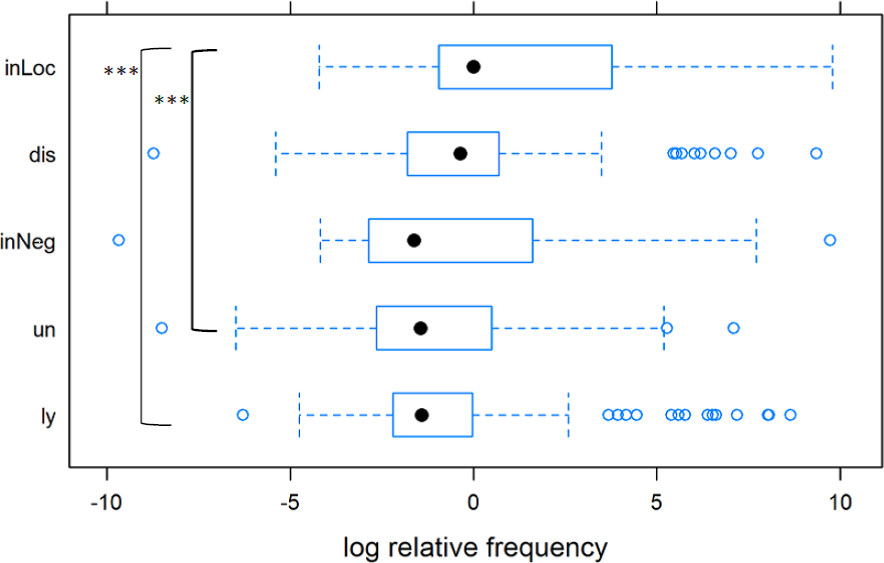
\includegraphics[scale=0.5]{images/Corpus/corpusComparisonRelFreq2.png}
	\caption{ Comparison of the relative frequency of the five affixes }
	\label{fig: corpus RelFreq comparison}

\end{figure*}


The plot suggests that locative \prefix{in} is the least segmentable affix having the highest relative frequency. It is followed by \prefix{dis}. The median relative frequencies of \prefix{in}, \prefix{un} and \suffix{ly} do not differ to a high degree, but the plot suggests that, with regard to their decomposability, \suffix{ly} and \prefix{un}affixed words are more uniform than words with negative \prefix{in}. In other words, while the majority of the \suffix{ly}- and \prefix{un}words have a rather low relative frequency, we find some variation with negative \prefix{in}. 
 An ANOVA ($F=6.716 ,p<0.001$) indicates that there is a significant difference between the relative frequency of the five affixes. Pairwise comparisons using Tukey contrasts reveal, however, that only two of the differences are significant. The affix with the highest relative frequency, locative \prefix{in}, is significantly different from the two affixes with the lowest relative frequency, \prefix{un} ($t$-$value=4.813, p<0.001$)  and \suffix{ly} ($t$-$value=4.489, p<0.001$). 

            

One reason for the insignificance of the contrasts between the affixes might be that there are not enough observations for each affix to reach significance. Furthermore, the differences in relative frequency between the affixes are quite small. This is partly due to the gradient nature of the variable log\textsc{RelativeFre-quency}. In combination, the size of the data set and the gradient nature of the variable might lead to a lack of statistical power. 
To alleviate this problem, I recoded the variable log\textsc{RelativeFrequency} into a categorical one. This especially makes sense considering that the variable has a natural threshold. For all types with a relative frequency below 0, the derivative is less frequent than its base. For all items having a relative frequency higher than 0, the opposite is the case. Therefore, items with a relative frequency below 0 were recoded as being `more decomposable', and items with a relative frequency higher than 0 were recoded as `less decomposable' (see \citealt{Hay.2001,Collie.2008} for a similar coding of relative frequency). \tabref{tbl:Corpus Categorical RelFreq} displays the distribution across affixes.
Pairwise comparisons revealed that \suffix{ly} has significantly more `more decomposable' words  than negative \prefix{in}, locative \prefix{in} and \prefix{dis}. Furthermore, locative \prefix{in} has significantly less  `more decomposable' words than \prefix{un} and negative \prefix{in}. 







% Summary Rel Freq
To sum up the comparisons of the affixes' relative frequency, \prefix{un} and \suffix{ly} are the most segmentable affixes, locative \prefix{in} is the least segmentable affix. The affixes \prefix{dis} and negative \prefix{in} seem to be in the middle of the scale. However, in both analyses (gradient and categorical relative frequency), only few contrasts proved to be significant.






\begin{table*}
	
	\caption{Categorical relative frequency by affix }
	\label{tbl:Corpus Categorical RelFreq}
	
		\resizebox{\textwidth}{!}{%
			\begin{tabular} {lrrrrrrrrrr}
				\lsptoprule
				\textsc{Cat. Relative}& & & &&   \\
				\textsc{Frequency }&\multicolumn{2}{c}{\prefix{in}\textsubscript{\textsc{Loc}}   }&\multicolumn{2}{c}  {\textit{dis-}} &   \multicolumn{2}{c} {\prefix{in}\textsubscript{\textsc{Neg}}   } &\multicolumn{2}{c} {\prefix{un} }& \multicolumn{2}{c} {\suffix{ly}  }  \\
				\midrule
				less    decomposable              &     38 &(70\%) &   30 &(48\%)   &  9 &(31\%)  & 35& (35\%)   &35& (23\%)        \\
				more decomposable &  16 &(30\%) &   32& (52\%)  &  20 &(69\%) &66& (65\%) & 115& (77\%) \\
				\lspbottomrule                                                                                
		\end{tabular}
		}
	
\end{table*}




\begin{figure*}
	
	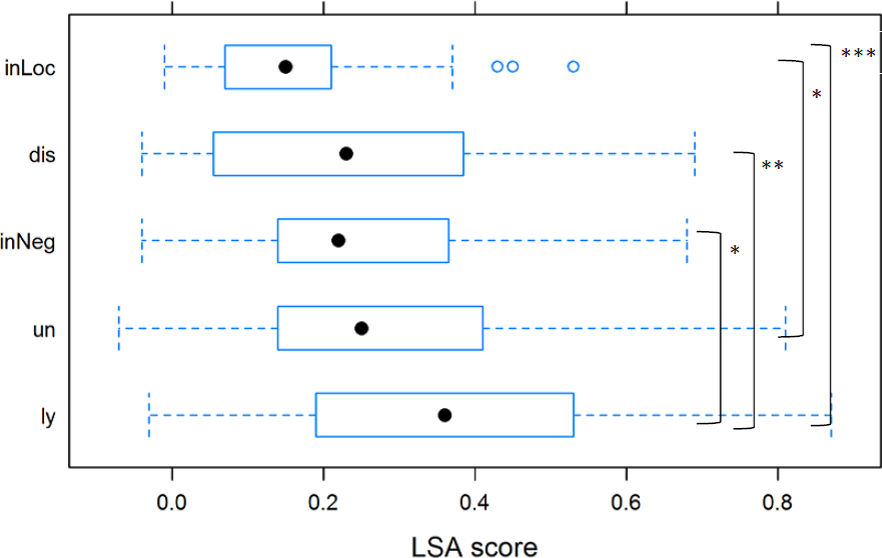
\includegraphics[scale=0.5]{images/Corpus/corpusComparisonLSAScores2.png}
	\caption{ Comparison of LSA score of the five affixes }
	\label{fig: corpus LSA comparison}
\end{figure*}


%  LSA
Turning to the last measure of decomposability, the comparison of the affixes' LSA scores reveals that there are only minor differences between the affixes. \figref{fig: corpus LSA comparison} displays these differences using boxplots. On the x-axis the LSA score is displayed. Each box represents the distribution of the LSA scores for one affix in increasing order. Locative \prefix{in} has the lowest score indicating that words featuring this affix are the least semantically similar to their base words. In terms of semantic similarity, they can thus be said to be the least decomposable words in the data set. Words with the affix \suffix{ly} have the highest score, and are thus the most similar to their base word. They are the most decomposable.
However, the figure shows that there is a big overlap in the distribution of the LSA scores across affixes, i.e. the differences between affixes are rather small. Statistical analyses confirm this impression.
While an ANOVA ($F=8.512, p< 0.001$) showed a significant effect of the affix on the LSA score, the pair-wise comparison of the means using Tukey contrasts shows  that only four of the contrasts are significant. The affix \suffix{ly} has significantly higher LSA scores than the affixes \prefix{un} ($t$-$value=0.027, p=0.01$), locative \prefix{in} ($t$-$value=5.197, p< 0.001$) and \prefix{dis}  ($t$-$value=3.443, p=0.006$). Furthermore, the affix \prefix{un} has significantly higher scores than the  affix locative \prefix{in} ($t$-$value=2.772, p=0.044$). 



        When interpreting the results for the variable \textsc{LSAScore}, it should be remembered that for some affixes not all items were taken into consideration in the comparisons. While for most of the \suffix{ly}- and \prefix{un}affixed words the LSA score could be computed (118 types for \suffix{ly}, 89 types for \prefix{un}), for the other affixes fewer types were considered in this comparison (between 23 and 40). Therefore, it is not surprising that we only find significant contrasts with \suffix{ly} and \prefix{un}, but not with the other affixes.  
        
        One can summarize that despite the fact that for a lot of types no LSA score could be computed, and the comparison of affixes in terms of their LSA score is thus based on a rather small number of observations, the distribution of the variable \textsc{LSAScore} reveals the same picture as the other decomposability variables. Locative \prefix{in} is the least segmentable affix, followed by \prefix{dis} and negative \prefix{in}. The affixes \prefix{un} and \suffix{ly} are the most segmentable affixes. 
        
                                                               
After having looked at each decomposability measure individually, let us now take a look at the whole picture. \tabref{tbl:summary comparison of affix} summarizes the results of the comparisons by showing a segmentability hierarchy for each decomposability measure. The segmentability hierarchies rank the affixes from the most segmentable to the least segmentable. The table shows very similar hierarchies for all measures. Locative \prefix{in} is the least segmentable affix, followed by \prefix{dis} and negative \prefix{in}. The affixes \prefix{un} and \suffix{ly} are the most segmentable affixes out of the five. 


\begin{table*}
	\caption{Segmentability hierarchies for each decomposability measure}
	\label{tbl:summary comparison of affix}
	
			\resizebox{\textwidth}{!}{%
		\begin{tabular} {lrcrcrcrcr}
			\lsptoprule
			\textbf{Decomposability measure}& & &&&&& &&\\
			\midrule
			\textsc{SemanticTransparency}  &\{\prefix{un} &, &\suffix{ly}\}  &>&   \prefix{in}\textsubscript{\textsc{Neg}}  &>&  \prefix{dis}  &>&\prefix{in}\textsubscript{\textsc{Loc}}  \\		
			
			\textsc{SemanticTransparencyRating }&\prefix{un}  &>& \suffix{ly}  &>&   \prefix{in}\textsubscript{\textsc{Neg}}   &>&\prefix{dis}  &>&  \prefix{in}\textsubscript{\textsc{Loc}}  \\	
			
			\textsc{TypeOfBase} &\{\prefix{un} &, &\suffix{ly}\}  &>&   \{\prefix{in}\textsubscript{\textsc{Neg}}  &,&  \prefix{dis}\}  &>&\prefix{in}\textsubscript{\textsc{Loc}}  \\	
			
			log\textsc{RelativeFrequency}&\suffix{ly} &> &  \prefix{un}  &> &   \prefix{in}\textsubscript{\textsc{Neg}}&> &  \prefix{dis}     &> &\prefix{in}\textsubscript{\textsc{Loc}}  \\				
			
			\textsc{Cat.RelativeFrequency}&\suffix{ly} &> &  \prefix{un}  &> &   \prefix{in}\textsubscript{\textsc{Neg}}&> &  \prefix{dis}     &> &\prefix{in}\textsubscript{\textsc{Loc}}  \\				
			
			\textsc{LSAScore}&\suffix{ly} &> &  \prefix{un}  &> &   \prefix{in}\textsubscript{\textsc{Neg}}&> &  \prefix{dis}     &> &\prefix{in}\textsubscript{\textsc{Loc}}  \\				
			
			\lspbottomrule                                                                                
		\end{tabular}
	}
	
\end{table*}



The differences  between the hierarchies mostly concern the ranking of \prefix{un} and \suffix{ly}. In terms of \textsc{LSAScore} and log\textsc{RelativeFrequency}, \suffix{ly} is more segmentable than \prefix{un}, in terms of \textsc{SemanticTransparencyRating}, \prefix{un} is more segmentable than \suffix{ly}, and in terms of \textsc{SemanticTransparency} and \textsc{TypeOfBase}, there is no difference between the two. 
While all hierarchies display a very similar picture, it is to note that they differ with regard to how significant differences between affixes are. While for \textsc{SemanticTransparency} and \textsc{TypeOfBase} all differences were significant, this was not the case for the other measures of decomposability. 


The results of the segmentability comparison fit in with previous research on the segmentability of prefixes. \cite{Zirkel.2010}, for example, investigated the parsability of 15 prefixes in terms of four different measures (productivity, type parsing ratio, token parsing ratio and average boundary strength). The comparison of the prefixes revealed that out of the 15 investigated prefixes, \prefix{un} is the third most segmentable, and \prefix{dis} is the 10th most segmentable. In other words, as in the present study, the prefix \prefix{un} is very segmentable and the prefix \prefix{dis} is far less segmentable. The prefix \prefix{in} was not investigated in \cite{Zirkel.2010}. 

Overall, the segmentability hierarchies displayed in \tabref{tbl:summary comparison of affix} match the Non-Semantic Segmentability Hierarchy. Thus, the Non-Semantic Segmentability Hierarchy is borne out by the data. This supports its validity and thus shows that the predictions made by the affix-specific Morphological Segmentability Approach are valid.

\subsection{Summary } \label{summary decomposability corpus study}

% Cluster analyses
In the first part of this section the relation between the five measures of decomposability \textsc{SemanticTransparency}, \textsc{SemanticTransparencyRating}, \textsc{TypeOfBase}, log\textsc{RelativeFrequency} and \textsc{LSAScore} was investigated. The cluster analyses revealed that the three variables \textsc{SemanticTransparency}, \textsc{SemanticTrans-parencyRating} and \textsc{TypeOfBase} are highly correlated. The two gradient measures  log\textsc{RelativeFrequency} and \textsc{LSAScore}  did not correlate with any other decomposability variable.  
One can thus summarize that, while  \textsc{SemanticTransparency}, \textsc{SemanticTransparencyRating} and \textsc{TypeOfBase} tap into the same phenomenon, and are therefore well suited to be used as operationalizations of the same concept, this cannot be said for 
log\textsc{RelativeFrequency} and \textsc{LSAScore}. 
It was argued that the results can be interpreted as evidence for three different types of decomposability. The first type is operationalized by  \textsc{SemanticTransparency}, \textsc{SemanticTransparencyRating} and \textsc{TypeOfBase}, the second by log-\textsc{RelativeFrequency}, and the third by \textsc{LSAScore}. Potential effects of the decomposability variables must be interpreted with these different types of decomposability in mind. 

 In the second part of the section, the distributions of the decomposability variables across affixes were compared. All comparisons revealed the same picture. Locative \prefix{in} is the least segmentable affix, \prefix{un} and \suffix{ly} are the most segmentable. The prefixes negative \prefix{in} and \prefix{dis} pattern in between. 
 Even though not all contrasts proved to be significant, and the categorical measures seemed to provide a clearer picture than the gradient measures, one can say that the decline in segmentability from \prefix{un} and \suffix{ly} to locative \prefix{in} is supported by all measures. 
 This order resembles the Non-Semantic Segmentability Hierarchy (cf. \figref{fig:Segmentability hierarchies of  affixes repetition 2} ). The corpus data thus empirically verifies one of the proposed segmentability hierarchies. In turn, the gemination prediction of the affix-specific Segmentability Approach, which is based on the Non-Semantic Segmentability Hierarchy, is valid. 

\section{Duration}


\subsection{Analyses} \label{analyses dur corpus}


The first durational analysis consists of investigating the distribution of consonant duration in each subset to test whether gemination is a categorical or a gradient phenomenon (cf. `Nature of gemination: Predictions' in \sectref{predictions nature of gemination}). To see whether the distributions significantly differ between environments, I generated boxplots for each environment of each subset and applied standard test statistics. 
If doubles show a significantly higher mean than singletons, and the boxplots indicate that the distributions of doubles and singles differ significantly, the data shows a bimodal distribution. In that case, one can assume gemination to be categorical. 
If there is no significant difference in the distribution of the environments, two explanations are possible. The first one is that the morphological geminates in the given data set degeminate, i.e. there is no difference in the duration of doubles and singles in the data set. The other possibility is that gemination is a gradient phenomenon which is not traceable by merely looking at distributions of durations and comparing averages. To check which of the two explanations holds, further statistical models are needed, i.e. linear regression models. 



I fitted at least two linear regression models for each subset, one predicting absolute consonant duration in milliseconds  (\textsc{AbsoluteConsonantDuration}) and one predicting relative consonant duration (\textsc{RelativeConsonantDuration}). Relative consonant duration refers to the duration of the consonant relative to the duration of the preceding vowel. In addition to the models for each subset, one model directly comparing the three prefixes with nasals, i.e. \prefix{un}, locative \prefix{in} and negative \prefix{in}, was fitted. While this model has the advantage of directly comparing the three prefixes with each other, it also faces several problems, such as the systematic difference in the distribution of variables between the prefixes. As will be discussed in the pertinent section, these problems limit the usefulness of the model to a great degree, e.g. some variables cannot be investigated in the model.

In the relative duration models, the independent variable \textsc{PrecedingSegmentDuration} was not included. This was because relative duration is computed by means of preceding segment duration. In other words, the variable \textsc{PrecedingSegmentDuration} is part of the dependent variable and therefore not a suitable predictor variable.


With regard to the decomposability measures, only in the \prefix{in} and \prefix{dis}models all five decomposability variables were included. In the \prefix{un} and \suffix{ly}-models, only the effects of log\textsc{RelativeFrequency} and \textsc{LSAScore} were tested. The reason is the distribution of the variables in the different subsets (see \sectref {The decomposability of the four affixes: a comparison} for discussion). 
Since the variable \textsc{LSAScore} was not coded for all items, i.e. the inclusion of the variable results in a loss of a lot of data points, the effect of this variable was tested individually in all subsets. 

In the models predicting consonant duration with \prefix{in} and \prefix{dis}, collinearity problems had to be addressed. As discussed in the previous section, the three decomposability variables \textsc{SemanticTransparency}, \textsc{SemanticTransparencyRating} and \textsc{TypeOfBase} highly correlate, and it was thus problematic to test all of them simultaneously in the model. Therefore, the effect of these variables was tested by including them individually in the model, and by conducting principal component analyses (cf. \sectref{stats}). 


The use of mixed effects models was precluded by the data's unnestedness. Almost every item is produced by a different speaker and many items occur only once in the corpus, so that it did not make sense to use speaker and item as random effects (see also discussion in \sectref{sampling corpus}). All models were fitted according to the modeling strategy described in \sectref{stats}.



All models were tested for two types of  interactions. First, I tested for interactions which are predicted to affect gemination according to the theoretical approaches discussed in chapter \ref{Theory}. These  are the interactions between the variable \textsc{Environment} and the decomposability variables, and the interaction between \textsc{Environment} and \textsc{Affix}.
Then, I tested for interactions which, based on previous empirical work and theoretical considerations, can be assumed to affect affixational consonant duration. In other words, I tested for interactions between variables for which one can assume that their relationship leads to a situation in which the simultaneous influence of the variables on affixational consonant duration is not additive. One of those interactions is, for example, the interaction between \textsc{Environment} and \textsc{BaseInitialStress}. For prefixed words, it can be assumed that base-initial stress affects the duration of a double consonant differently than the duration of a singleton. The reason is that, as discussed in \sectref{Phonological representation of geminates}, part of the double consonant belongs to the base-initial syllable, while the singleton only belongs to the prefix. 
Some interactions were not testable because some level combinations were not attested. An example of such an untestable interaction is the interaction between \textsc{Environment} and \textsc{BaseInitialStress} in the \prefix{un}data set. There are no \prefix{un}prefixed words with a double consonant and an unstressed base-initial syllable. All interactions tested in the corpus study are listed in \hyperref[Appendix C: Summaries of tested interactions in corpus study]{appendix C}.

After fitting the regression models for each subset, I used multi-model inferencing to verify the results, i.e. to ensure that multi-model inferencing predicts the same variables to be important for predicting consonant duration as the final regression model (see \sectref{stats} for a discussion of multi-model inferencing).




The plots of the regression models were generated with the \texttt{visreg package} (\citealt{Breheny.2015}). For a plot showing the effect of a variable, all other variables are held constant at the median (for numeric variables) or at the most common category (for factors). For the models predicting absolute consonant duration, the plots always show the response variable \textsc{AbsoluteNasalDuration} in milliseconds, i.e. in cases where the dependent variable had to be transformed in the modeling process, the plots show the back-transformed variable.



\subsection{Overview}\label{overview corpus}



\begin{figure*}[t!]
	
		
		
		\begin{subfigure}
			
			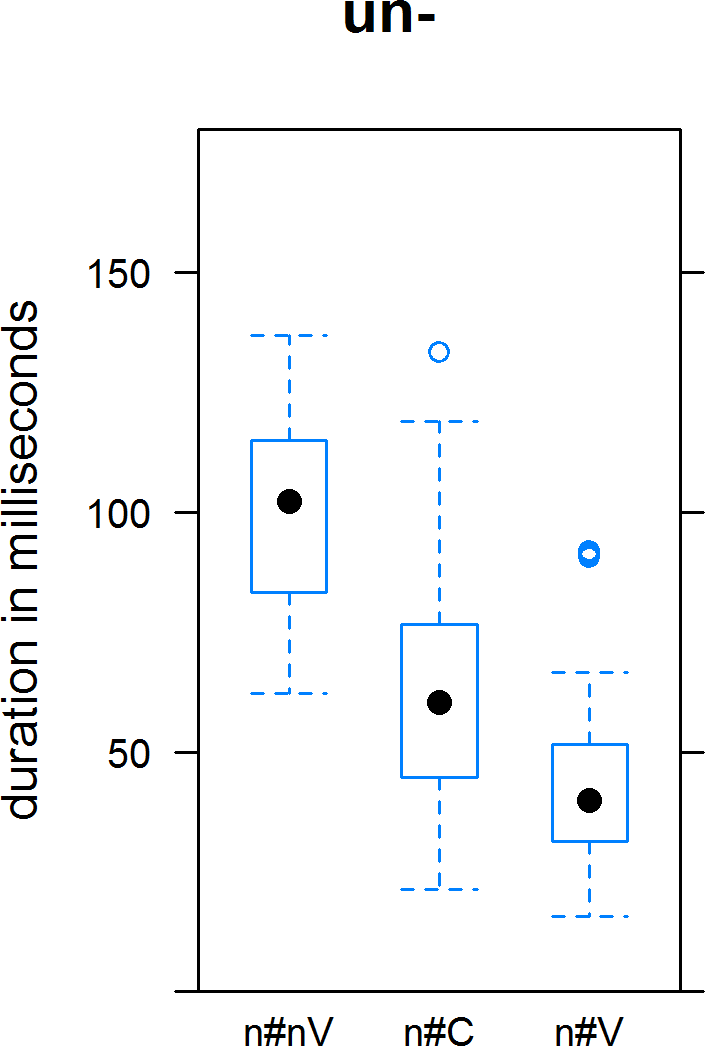
\includegraphics[scale=.55]{images/Corpus/boxUn.png}
			%	\caption{1a}
			%	\label{fig:sfig1}
		\end{subfigure}%
		~
		\begin{subfigure}
			
			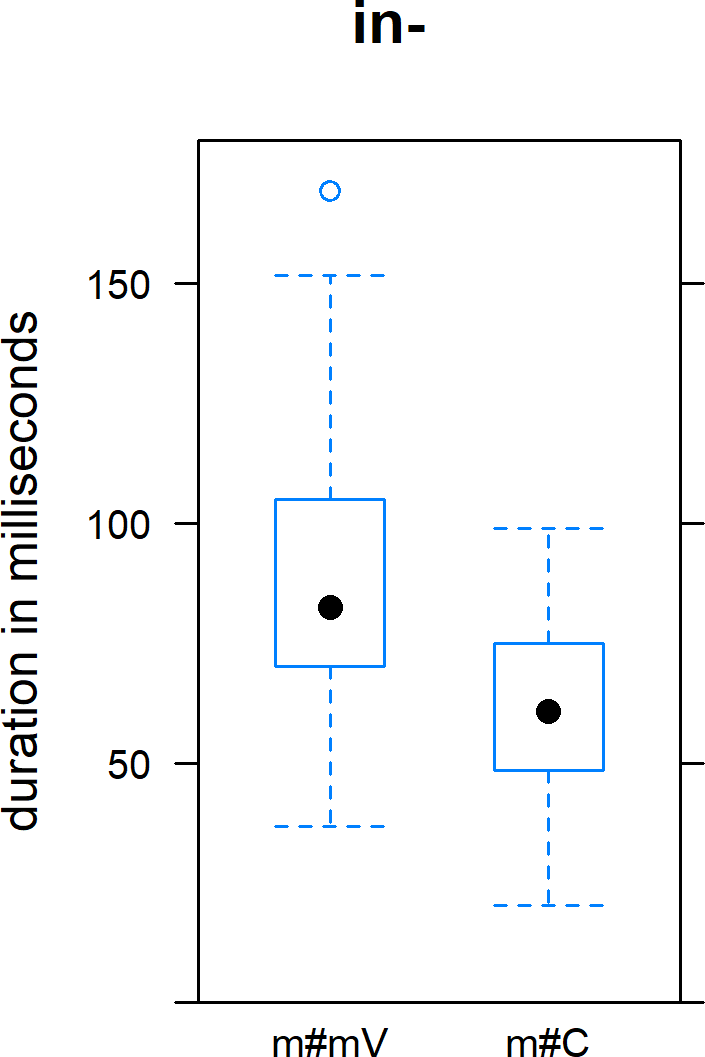
\includegraphics[scale=.55]{images/Corpus/boxIn.png}
			%	\caption{1b}
			%	\label{fig:sfig2}
		\end{subfigure}
		
		\begin{subfigure}
			
			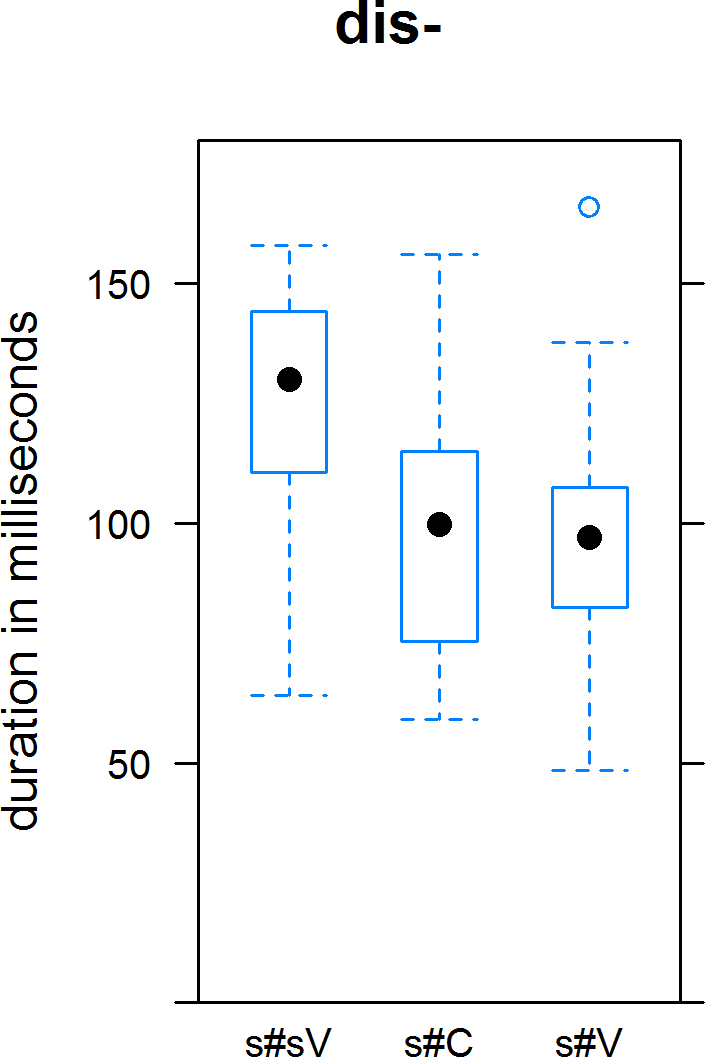
\includegraphics[scale=.55]{images/Corpus/boxDis.png}
			%	\caption{1b}
			%	\label{fig:sfig2}
		\end{subfigure}
		~
		\begin{subfigure}
			
			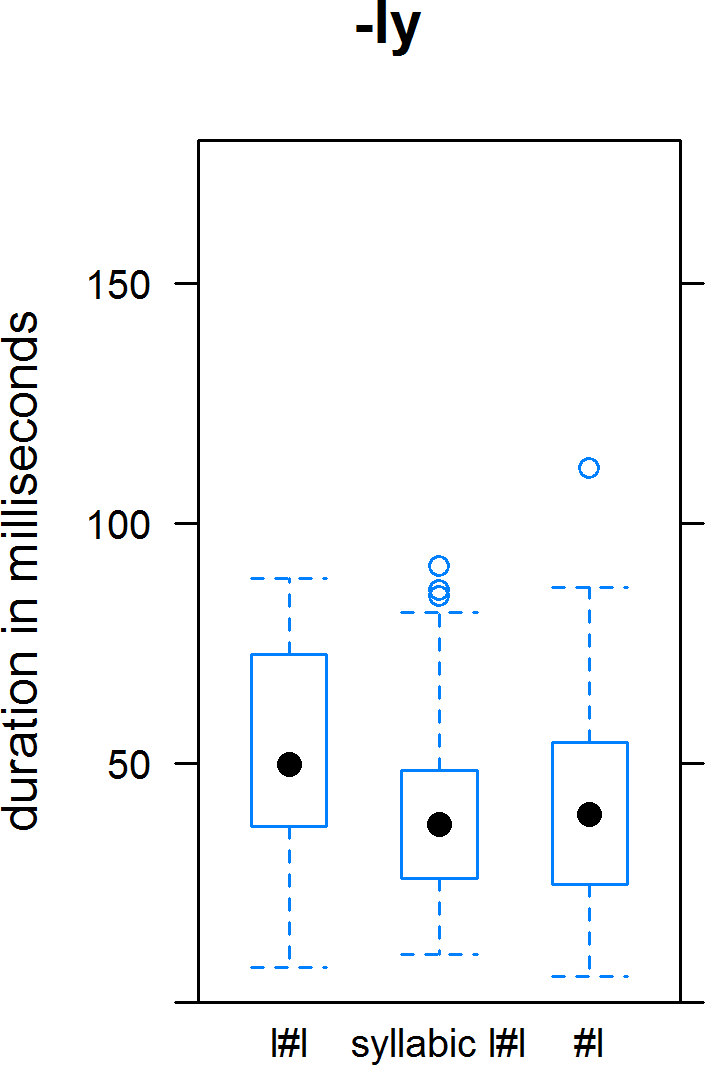
\includegraphics[scale=.55]{images/Corpus/boxLy.png}
			%	\caption{1b}
			%	\label{fig:sfig2}
		\end{subfigure}				
					
	\caption{Distribution of consonant duration in the four data sets}
	\label{fig:Corpus raw duration distribution}
\end{figure*}

% boxplots			
\figref{fig:Corpus raw duration distribution} depicts the distribution of consonant duration for each environment in each subset using boxplots. The distribution in the \prefix{un}data set is shown in the upper left panel, the one for \prefix{in} in the upper right panel, the one for \prefix{dis} in the lower left panel, and the one for \suffix{ly} in the lower right panel.
The y-axis of each plot displays the duration of the consonant in milliseconds. The leftmost box in each plot represents the distribution for items with a double consonant, and the boxes on the left show the distributions for items with a single consonant. For \suffix{ly}, the box in the middle of the panel shows the distribution of the syllabic doubles.
 
 
For the prefixes, the figure shows a clear difference in duration between double and single consonants. Doubles are longer than singletons. The figure also shows that there is a clear binary distribution in the \prefix{un}, \prefix{in} and \prefix{dis}data sets.  For \prefix{in} and \prefix{dis}, there is hardly any overlap in the interquartile range of doubles and singletons. For \prefix{un}, there is no overlap at all. For the prefixes, the durational distribution thus suggests a clear categorical difference between doubles and singletons. In other words, the plots suggest that the prefixes geminate, and that gemination is a categorical phenomenon. 
The \suffix{ly}-data set does not show a bimodal distribution, i.e. there is a big overlap in the distribution of doubles and singletons, and doubles are not significantly longer than singletons in this data set. One might thus suspect degemination for \suffix{ly}. Further statistical analyses are, however, necessary to confirm this impression.











  
  \begin{table*}
  	\caption{Duration of consonant(s) in milliseconds per environment for all affixes}
  	\label{tbl:Corpus raw duration}
  	
  		\begin{tabular} {lllll}
  			\lsptoprule
  			\textbf{un-}\\
  			%\\
  			Environment & Example & Mean & Median& Standard Deviation\\
  			\midrule			
  			n\#nV&\color{lsMidBlue}\textit{unnatural} & 100 & 102 & 21\\ 
  			n\#C&\color{lsMidBlue}\textit{untold} & 64 & 60 & 24\\ 
  			n\#V&\color{lsMidBlue}\textit{uneven} & 45 & 40 & 18\\
  			\midrule   	
  			Overall &  & 60 & 54 & 28\\ 
  			\midrule
  			%\midrule
  			\\
  			\textbf{in-}\\
  			%\\
  			
  			Environment & Example & Mean & Median& Standard Deviation\\
  			\midrule			
  			m\#mV&\color{lsMidBlue}\textit{immortal} & 87 & 81 & 27\\   	
  			m\#C&\color{lsMidBlue}\textit{impossible} & 61 & 61 & 19\\ 
  			\midrule   	
  			Overall &  & 76 & 74 & 27\\ 
  			\midrule   
  			%\midrule
  			\\
  			\textbf{dis-}\\
  			%\\
  			Environment & Example & Mean & Median& Standard Deviation\\
  			\midrule			
  			s\#sV&\color{lsMidBlue}\textit{dissatisfied} & 127 & 130  &35 \\ 
  			s\#C&\color{lsMidBlue}\textit{disgrace} & 100 & 100& 29\\ 
  			s\#V&\color{lsMidBlue}\textit{disarm} &95 & 96 & 22 \\ 
  			\midrule   	
  			Overall &   &103   & 102  & 30  \\ 
  			\midrule   	
  			%\midrule
  			\\
  			\textbf{-ly}\\
  			%\\
  			\midrule
  			Environment & Example & Mean & Median& Standard Deviation\\
  			\midrule			
  			l\#l&\color{lsMidBlue}\textit{really} & 50  & 50 & 23 \\ 
  			syllabic l\#l&\color{lsMidBlue}\textit{ment(a)lly} &41 & 37  & 21\\ 
  			\#l&\color{lsMidBlue}\textit{possibly} & 42& 39& 21\\ 
  			\midrule   	
  			Overall &  &43  &41 &22\\ 
  			\lspbottomrule                                                                                
		\end{tabular}
  	
  \end{table*}
  

\tabref{tbl:Corpus raw duration} shows a summary of the distribution of consonant duration for each environment in the four subsets. Overall the durations of the consonants in the data set are in the same range as those found in other studies. For example, \citet[Tables II and X]{Umeda.1977} finds in her North American English data that intervocalic word-internal singleton /n/ is between 34 and 38 ms long (depending on stress). 
Double /n/s across a word boundary have a duration of 100 ms. For singleton intervocalic word-medial /m/, Umeda finds mean durations between 70 and 74 ms, and for singleton /s/, mean durations range from 90 to 120 ms in that position. Singleton /l/ is between 40 and 47 ms long in Umeda's study. This indicates that the data and the durational measurements are valid.

Let us now turn to the distribution of duration for single and double consonants in the data, i.e. to the question of gemination.  As already shown in \figref{fig:Corpus raw duration distribution}, for the three prefixes the mean and median duration of the double consonants is much higher than the mean and median duration of the single consonants. The differences in mean range from 26 ms (\texttt{m\#mV} to  \texttt{m\#C)} to 55 ms (\texttt{n\#nV} to  \texttt{n\#V}). For \suffix{ly}, there is a difference in mean duration of 8 ms between double /l/ (\texttt{l\#l}) and single /l/ (\texttt{\#l}). The double is thus only slightly longer than the singleton.
  
  


% stats for doubles vs. singles

To get a first idea about the nature of these differences between environments, some univariate analyses were carried out. The pair-wise comparison of the means for \prefix{un} using Tukey contrasts yields significant contrasts for all three pairs, i.e. the differences between all environments are significant (see \tabref{tbl:Tukey un}). This suggests gemination for \prefix{un}. 
For \prefix{in}, a Welch t-test shows a significant difference between the two environments \texttt{m\#mV} and \texttt{m\#C} ($t$($152.98$) $=7.1122$, $p< 0.001$). 
Thus, as in the \prefix{un}data set, in the \prefix{in}dataset doubles are significantly longer than singletons.
For \prefix{dis}, the comparison of the means also yields significant contrasts for the difference between doubles and singletons (see \tabref{tbl:Tukey dis}). However, the difference between the two singleton levels is not significant. None of the differences between the \suffix{ly}-environments proved to be significant. Thus, while for all the prefixes, doubles are significantly longer than singletons, this is not the case for the suffix \suffix{ly}.


  \begin{table*}
  	\caption{Multiple comparison of means of nasal duration for \prefix{un}prefixed words (Tukey contrasts)}
  	\label{tbl:Tukey un}
  	
  		\begin{tabular} {lrrrr}
			
			
			\lsptoprule
  			& Estimate & Std. Error & $t$-value  & Pr($>$$|$$t$$|$)    \\
  			\midrule
  			n\#C - n\#nV  &-35  &  5 & -6.903 & $<$ 0.001\\
  			n\#V - n\#nV & -56 &  5 & -10.798 & $<$ 0.001\\
  			n\#C - n\#V  & -20 & 4 & -5.487 & $<$ 0.001 \\
  			\lspbottomrule                                                                                
		\end{tabular}
  	
  \end{table*}
  
  
  
  \begin{table*}
  	\caption{Multiple comparison of means of consonant duration for \prefix{dis}prefixed words (Tukey contrasts)}
  	\label{tbl:Tukey dis}
  	
  		\begin{tabular} {lrrrr}
			
			
			\lsptoprule
  			& Estimate & Std. Error & $t$-value  & Pr($>$$|$$t$$|$)    \\
  			\midrule
  			s\#C - s\#sV  &  - 28 &  7  & -6.903 & 0.001\\
  			s\#V - s\#sV & -32  &  7  & -10.798 &$<$ 0.001\\
  			s\#C - s\#V    &  {5}       &  5  &  -0.858  &  0.666  \\
  			  			\lspbottomrule                                                                                
		\end{tabular}

  	
  \end{table*}
  
  

					

All in all, the first analyses of durations have shown that the singleton consonant durations in the data are similar to the ones found in previous studies and the data is thus valid. Furthermore, the investigation of distributions suggests that the investigated prefixes geminate and that gemination is categorical. It also suggests degemination for \suffix{ly}. 
However, since it is well known that the duration of segments in natural speech is subject to a variety of different influences, more advanced statistical analyses are necessary to investigate the matter. In the next subsections I will present such analyses for each subset.



\subsection{The prefix \prefix{un}} \label{un corpus}

\subsubsection{Absolute duration}

The linear model predicting absolute duration with \prefix{un} was fitted according to the procedure described in sections \ref{stats} and \ref{analyses dur corpus}. 
The residuals of the initial model showed a non-normal distribution. Therefore, the dependent variable \textsc{AbsolutConsonantDuration} was transformed by the Box-Cox-transformation parameter $0.303$, and outliers were removed. The removal of outliers resulted in the loss of  2 observations, i.e. 1.3\% of the observations. After the model was refitted with the transformed dependent variable, it showed a satisfactory distribution of residuals. The model was then simplified and interactions were tested  (see \hyperref[Appendix C: Summaries of tested interactions in corpus study]{appendix C} for a list of all tested interactions).
None of the interactions was significant, and only two significant predictors remained in the final model, \textsc{Environment} and  \textsc{LocalSpeechRate}. The model explains 57\% of the variance found in the data. \tabref{tbl: summary model un} documents the estimates for each predictor and their p-values in the final model.

\begin{table*}[!h]
	\caption{Summary of linear model for variables predicting the Box-Cox-transformed duration of [n] in \prefix{un}prefixed words}
	\label{tbl: summary model un}
	
		
		
		\begin{tabular}{lrrrr}
			
			
			\lsptoprule
			& Estimate & Std. Error & t-value & p-value  \\ 
			\midrule
			Intercept                           &   0.580 &  0.015  & 38.502 &  $<$ 0.001\\
			\textsc{Environment}-\texttt{n\#C} & -0.050 &  0.010 & -5.072 & $<$ 0.001\\
			\textsc{Environment}-\texttt{n\#V} & -0.097 &   0.010 & -9.770 & $<$ 0.001\\
			\textsc{LocalSpeechRate} &                 -0.008  & 0.001 &  -6.814 & $<$ 0.001\\
			
			\midrule\\
			Adjusted R-squared: 0.562  \\
			\lspbottomrule
		\end{tabular}

	
\end{table*}


\figref{fig:SpeechRate un} depicts the effect of \textsc{LocalSpeechRate}.  The y-axis of the graph displays the duration of the nasal in milliseconds, the horizontal axis represents the local speech rate. The line represents the estimated effect of the variable. The shaded areas in the graphs represent the 95\% confidence intervals. The  plot shows, the higher the speech rate, i.e. the more segments are pronounced in a given amount of time, the shorter becomes the nasal. This is an expected effect.





\begin{figure*}
	

	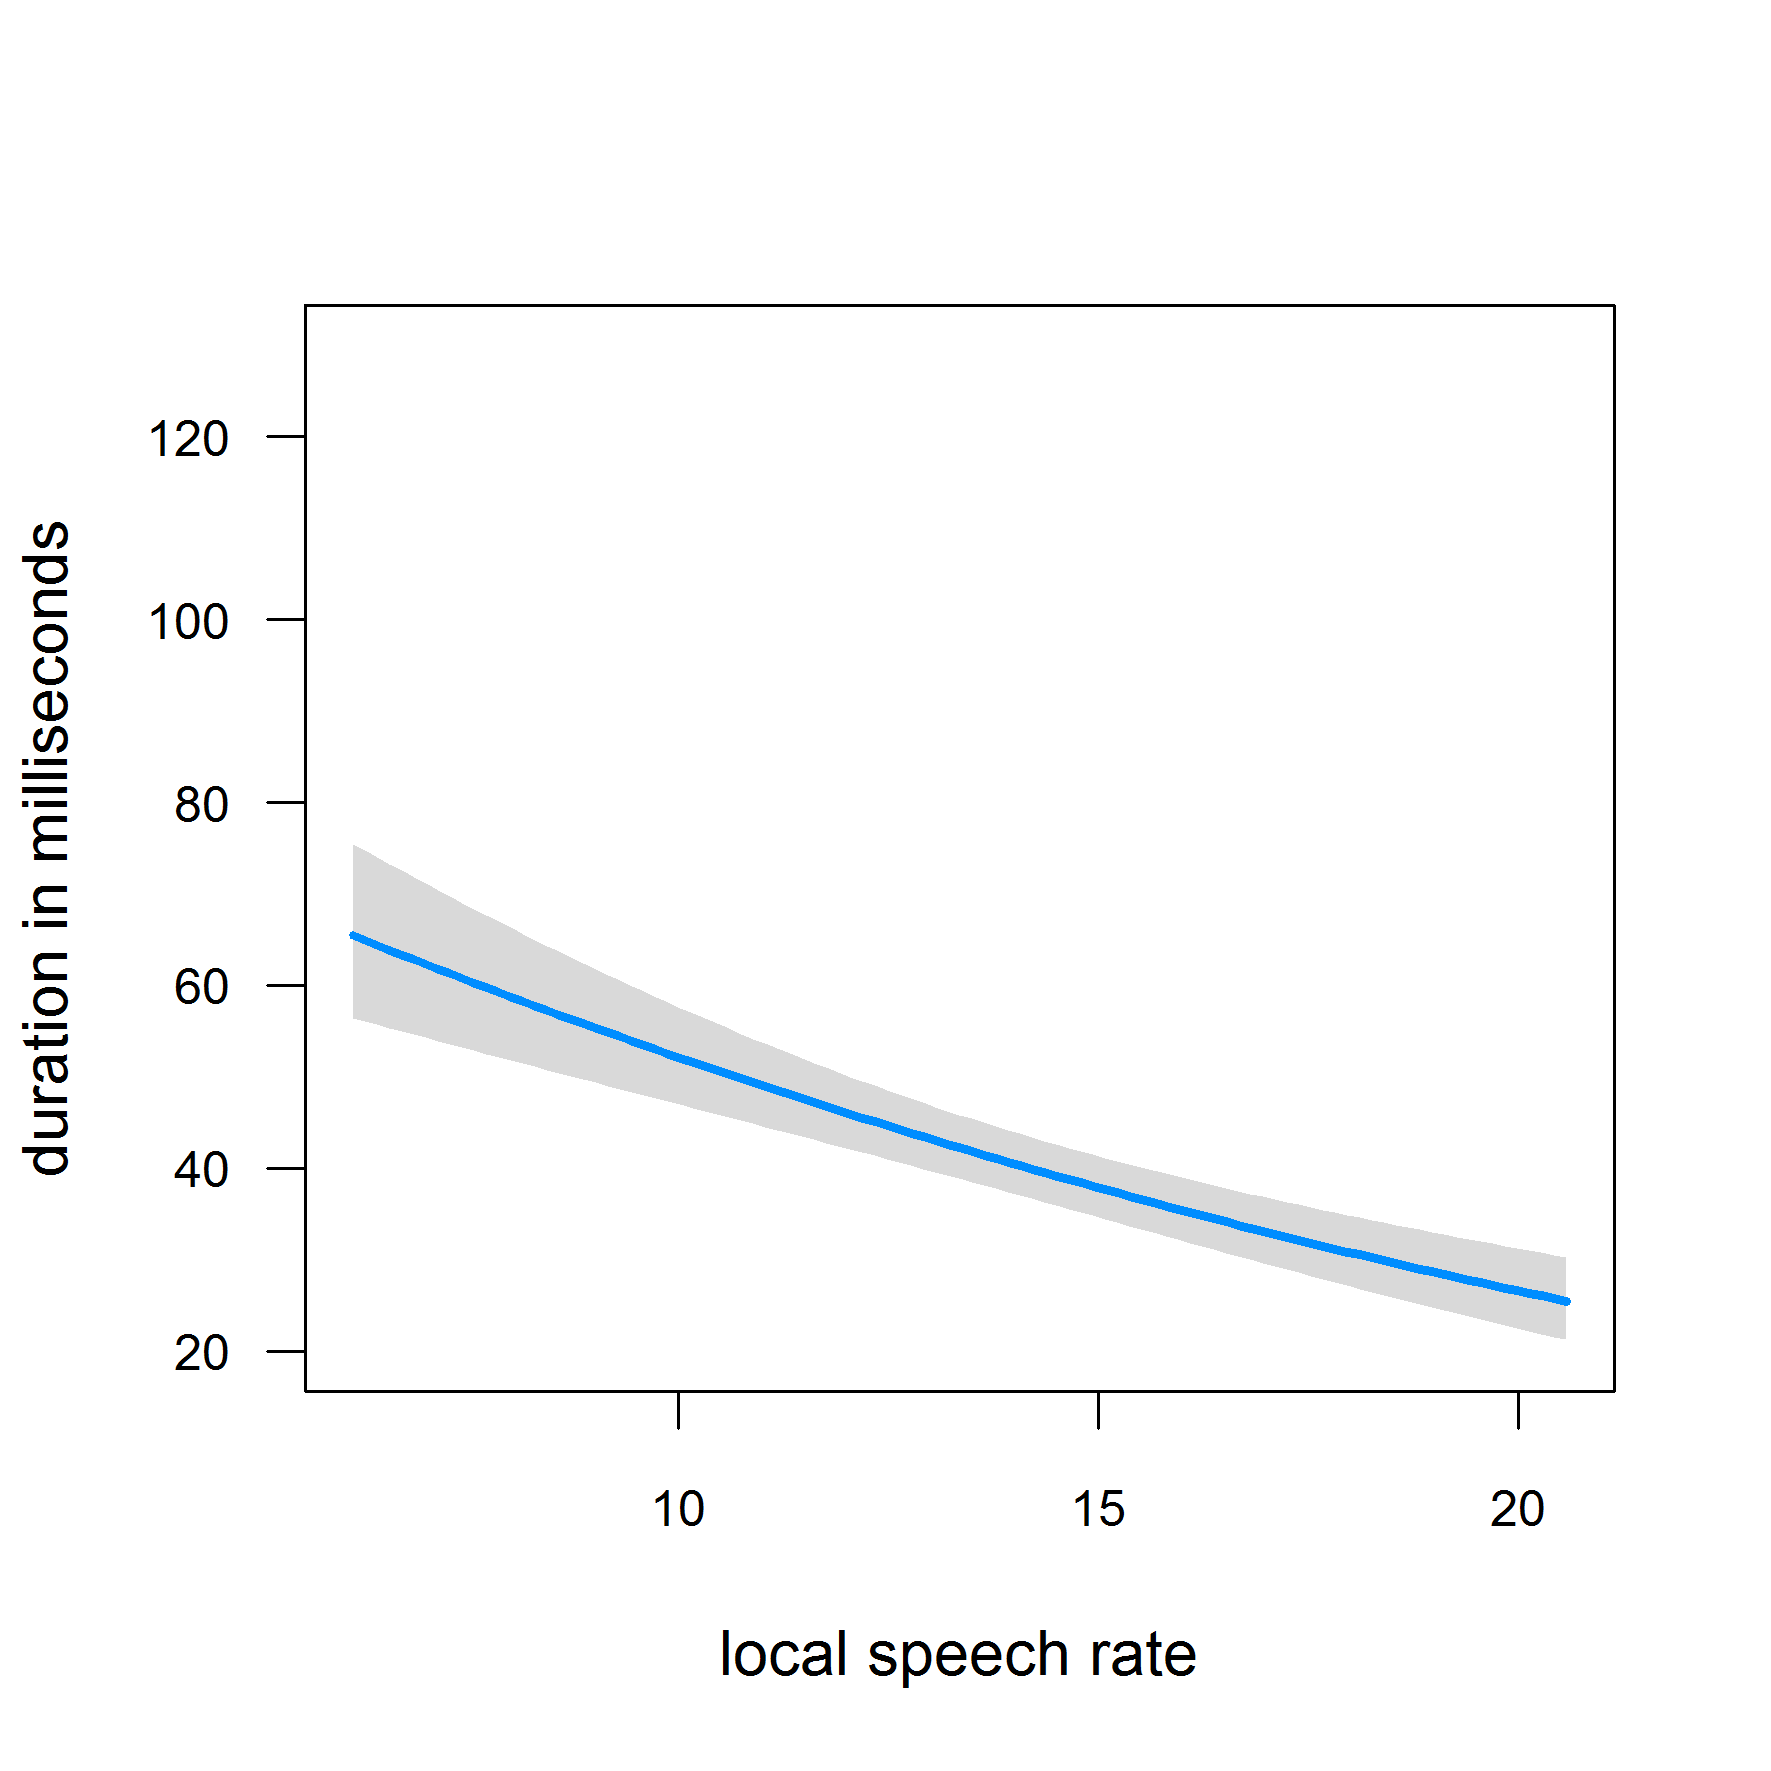
\includegraphics [scale=0.4]{images/Corpus/unModelSpeechRate.png}
	\caption{ Effect of local speech rate on consonant duration in \prefix{un}data set}
	\label{fig:SpeechRate un}

\end{figure*}





Let us now turn to our variable of interest, \textsc{Environment}. Its effect is shown in \figref{fig:NumNasal un}. The blue lines in the figure represent the estimated consonant duration for each of the three investigated environments. The graph shows that words containing a double nasal have a significantly longer duration than words with one nasal, no matter whether the single nasal is followed by a non-nasal consonant or by a vowel. In the case of a following vowel, the single /n/ is shortest. 




\begin{figure}  
	
	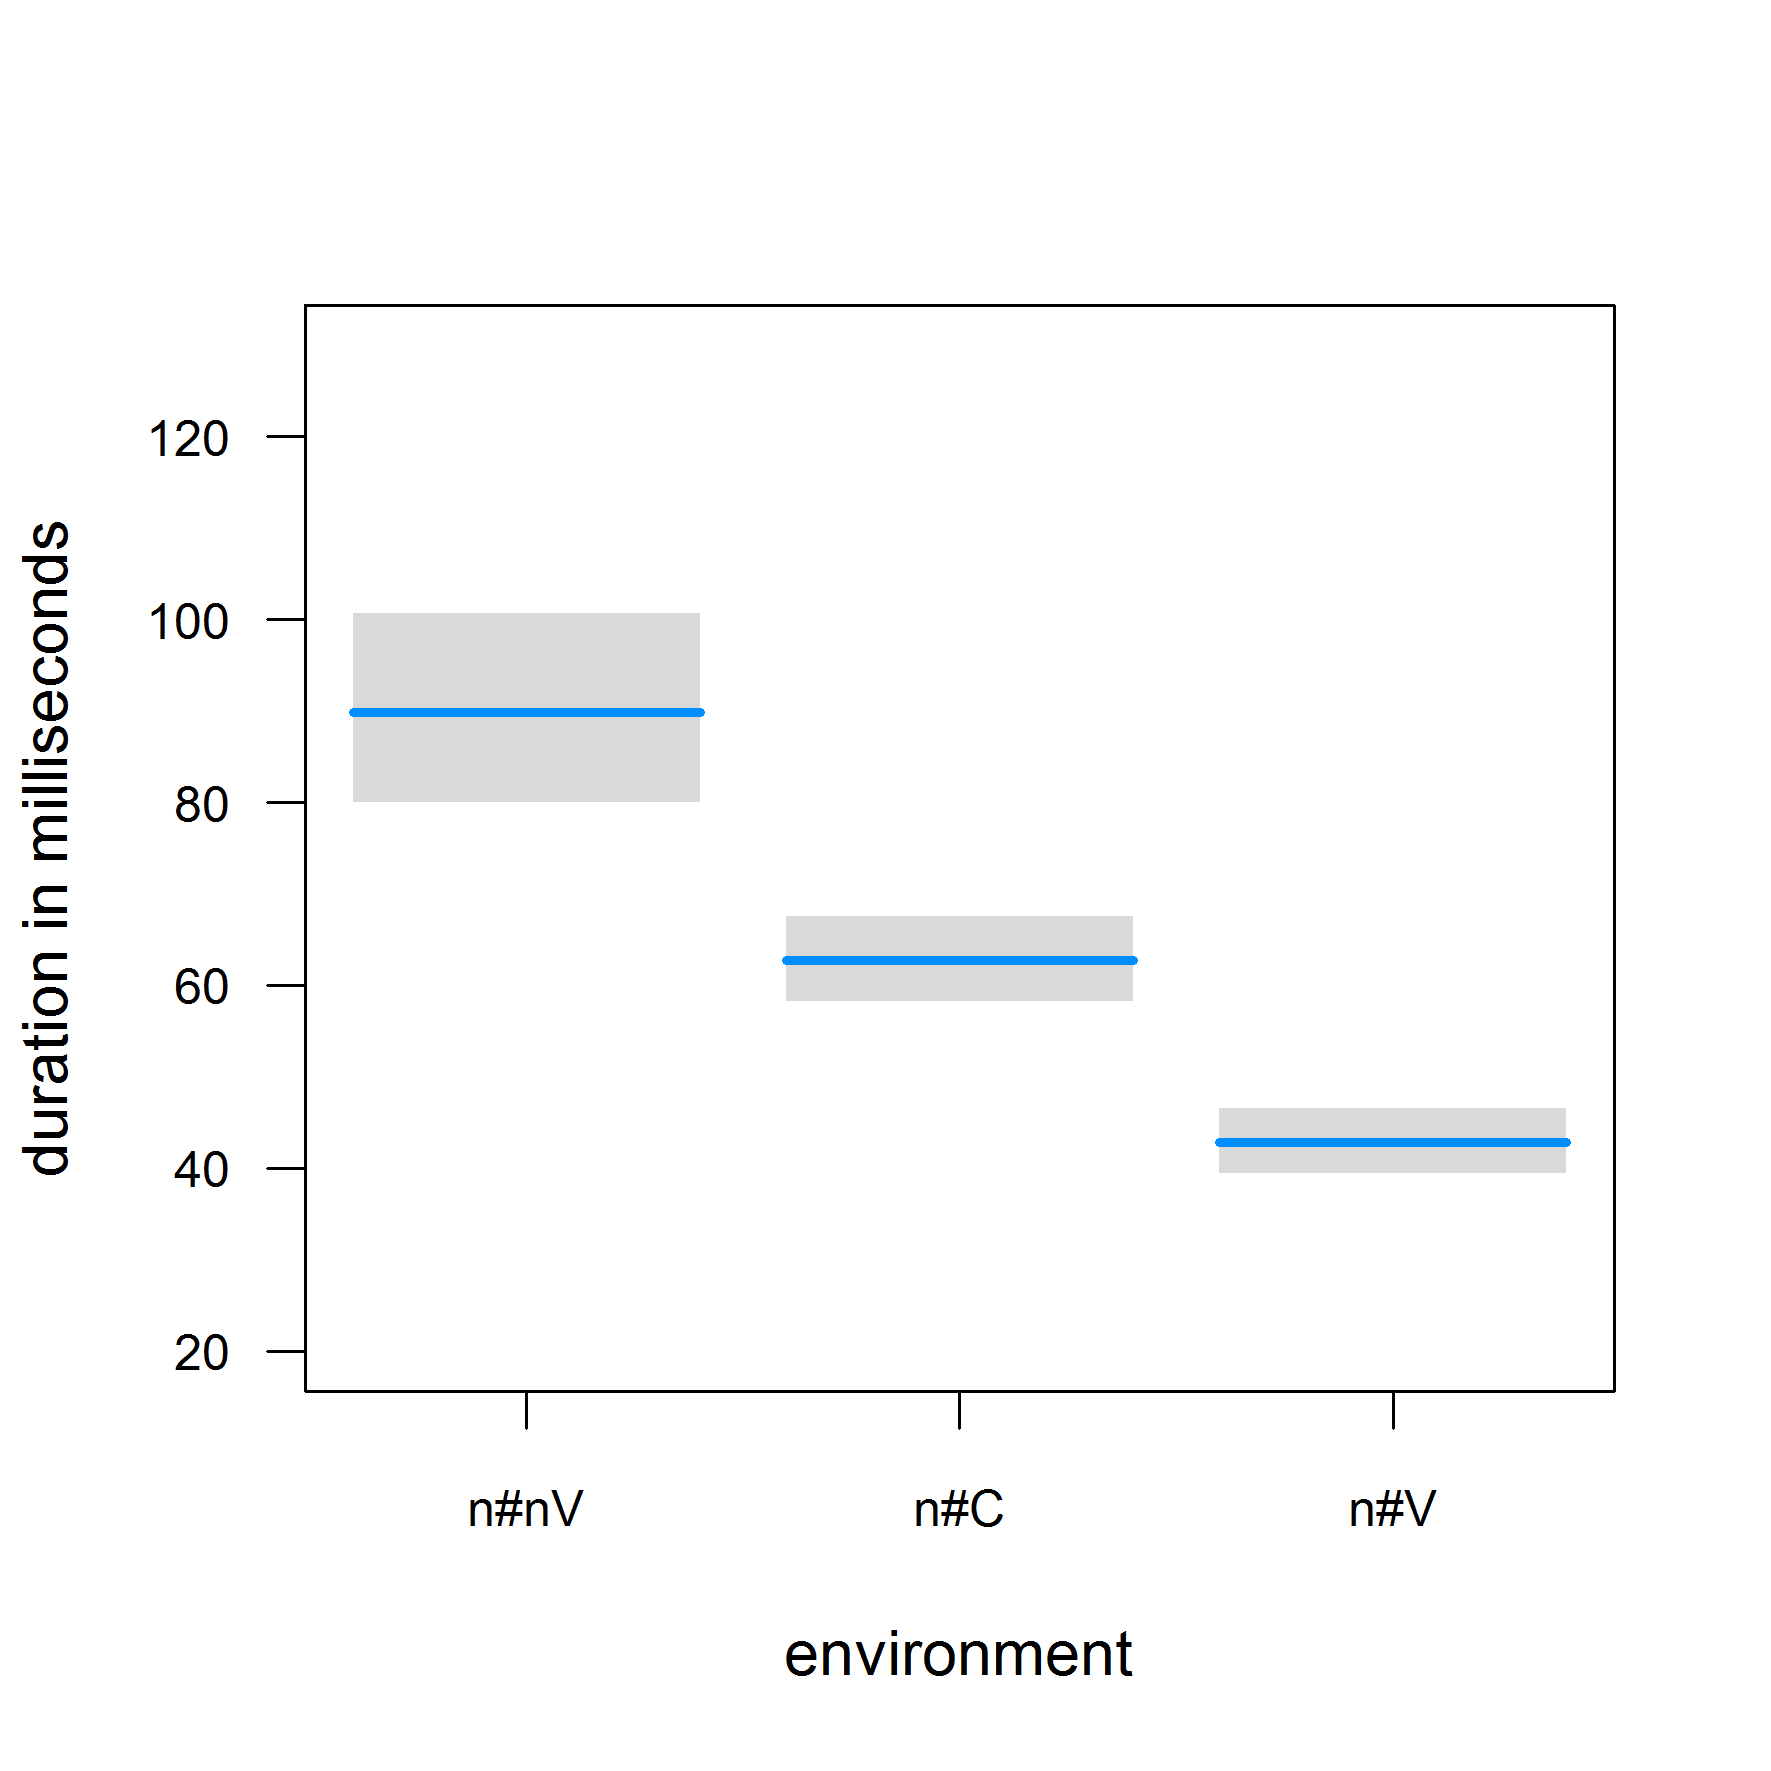
\includegraphics [scale=0.4] {images/Corpus/unModelNumNasal.png}
	\caption{Effect of environment on consonant duration in \prefix{un}data set}
	\label{fig:NumNasal un}
\end{figure}




The predicted mean duration for double nasals is 90~ms. For words with the \texttt{n\#C} environment the nasal is predicted to be 63~ms long, and for words having the \texttt{n\#V} environment it is predicted to be 43~ms long. If we compare the two environments with a following vowel (and thus hold the type of following segment constant), the model predicts double nasals to be even a bit longer than twice the duration of the average single nasal in this environment (90~ms as against 43~ms). This result clearly speaks in favor of gemination with \prefix{un}.

When a consonant follows the single nasal at the morpheme boundary, we also find a highly significant contrast between the two environments, but the difference is smaller. We do not find twice the duration for the double nasal, but only a difference of 27 ms, i.e. an increase in duration of 43\% from single to double nasal. 

The question may be raised whether this increase in phonetic duration can be interpreted as gemination in spite of the fact that the duration is not doubled. The literature on gemination has shown, however, that the durational differences between geminates and their corresponding singletons may vary substantially (see \sectref{what is gemination} for discussion). 
For /n/ in English, differences between 34\% and 109\% were found. For word boundary geminates, \cite{Delattre.} finds  an increase from singleton to geminate /n/ of 50\%.  All investigated environments in \citeauthor{Delattre.}'s study were were, however, vowel-initial.  For normal speech, \citet[86, Figure 2]{Oh.2012} arrive at an estimated 82~ms for word-internal singletons, 110~ms for \prefix{un}geminates and geminates across word boundaries. This is an increase of 60\%. For careful speech, they find estimated durations of 110~ms for singletons, 225~ms for \prefix{un}geminates, and 230~ms for geminates across word boundaries. This is an increase of 104\% to 109\%.\footnote{\citet{Oh.2012} do not give the estimated means in their article. The figures given here are read off from the partial effects plot given in Figure 2 of their article.} Note that again, only vocalic environments were tested.

The comparison to previous findings on gemination with English /n/ shows that there is good reason to interpret even the smaller of the two contrasts in the data (i.e. the one between \texttt{n\#C} vs. \texttt{n\#nV}) as evidence for gemination. While some studies have found bigger singleton-geminate ratios, some found smaller ratios. Differences in experimental set-up, especially speech condition, and  environment might be the cause of the different ratios found. In this study, the smaller singleton-geminate ratio between pre-consonantal singletons and doubles  (as against the ratio of pre-vocalic singletons and doubles) can be attributed to the type of following segment (C vs. V). As discussed in \sectref{variables of interest}, following consonants generally lead to longer durations for nasals.

After fitting the linear model, multi-model inferencing was used to detect which of the variables included in the initial model are the most predictive variables across a multitude of models. The variable \textsc{LSAScore} was not included in the multi-model inferencing analysis because of the low number of items which were coded for \textsc{LSAScore}. 
The analysis revealed that the two most important variables are those which also ended up in the final linear model, i.e. \textsc{Environment} (importance value: $1$) and \textsc{LocalSpeechRate} (importance value: $1$).  The importance values of the other variables are much lower (\textsc{PrecedingSegment-Duration}:  $0.4$, \textsc{BaseInitialStress}: $0.29$, log\textsc{WordFormFrequency}: $0.27$, log\textsc{Re-lativeFrequency}: $0.33$). This indicates that these variables are far less predictive of nasal duration than \textsc{Environment} and \textsc{LocalSpeechRate}. 


\subsubsection{Relative duration}


The model predicting relative consonant duration with \prefix{un} was fitted similarly to the model predicting absolute consonant duration and the same interactions were tested. Again the dependent variable was transformed using Box-Cox- transformation to achieve a normal distribution of residuals. The transformation parameter was $0.141$. In contrast to the absolute duration model, no outliers had to be excluded. 
 \tabref{tbl: summary corpus un rel dur} summarizes the final model. The model explains about 33\% of the variance and features only one variable, \textsc{Environment}.



\begin{table*}
	\caption{ Summary of linear model for variables predicting the Box-Cox-transformed relative duration of [n] in \prefix{un}prefixed words}
	\label{tbl: summary corpus un rel dur}
	
		
	\resizebox{\textwidth}{!}{%		
		\begin{tabular}{lrrrr}
			
			
			\lsptoprule
			& Estimate & Std. Error & t-value & p-value  \\ 
			\midrule
			
			Intercept       & 1.029  &0.013 & 80.326  &   	$<$ 0.001\\ 
			
			\textsc{Environment}-\texttt{n\#C}  &-0.072 &  0.015  &-4.858 & $<$ 0.001\\ 
			
			\textsc{Environment}-\texttt{n\#V}    &-0.127  & 0.015 &  -8.527 &   $<$ 0.001\\ 
			
			\midrule\\
			Adjusted R-squared:  0.327 \\
			\lspbottomrule
		\end{tabular}
}		
	
\end{table*}



The model reveals that, as in absolute duration, double /n/ is significantly longer than both singleton /n/s in relative duration. It thus confirms the results of the absolute duration model, i.e. \prefix{un} geminates. In contrast to the absolute duration model, the variable \textsc{LocalSpeechRate} is not significant in this model. This is not surprising, as the dependent variable \textsc{RelativeConsonantDuration} does not measure duration per se, but the relation of consonant duration and preceding vowel duration, i.e. a ratio. While speech rate is known to affect absolute duration, an effect on relative duration is not expected. 

Multi-model inferencing confirms the final model. The variable \textsc{Environment} is the most predictive variable (importance value: $1$). All other variables have very low importance values  (log\textsc{WordFormFrequency}: $0.56$, \textsc{BaseInitialStress}: $0.46$, \textsc{LocalSpeechRate}: $0.26$, log\textsc{RelativeFrequency}: $0.26$).


\subsubsection{Summary}

Two models were fitted to predict consonant duration with  \prefix{un}. The model predicting absolute consonant duration explains more variance than the one predicting relative consonant duration, i.e. the absolute duration model is the better model. In the absolute duration model, the noise variable \textsc{LocalSpeechRate} had the expected effect. In the relative duration model, no noise variables remained in the final model.
 Both models found a significant effect of the variable \textsc{Environment}. Phonological doubles (\texttt{n\#nV}) are significantly longer than phonological singletons, irrespective of whether the following segment is a consonant (\texttt{n\#C}) or a vowel (\texttt{n\#V}). The durational difference between doubles and singletons is more pronounced when the singleton is followed by a vowel, i.e. a following consonant lengthens the prefixal /n/. The results clearly show that the prefix \prefix{un} geminates.
With regard to the other variables of interest, only \textsc{LSAScore} and log\textsc{RelativeFrequency} could be tested. Neither had a significant effect. 


\subsection{The prefix \prefix{in}} \label{in corpus}


\subsubsection{Absolute duration}

The initial \prefix{in}model predicting absolute duration showed a non-normal distribution of residuals. Therefore, the dependent variable was  transformed (Box-Cox-transformation  parameter: $0.465$). After the transformation, the model showed a satisfactory distribution of residuals. The model was then fitted according to the strategy described in \sectref{stats} and interactions were tested (see \hyperref[Appendix C: Summaries of tested interactions in corpus study]{appendix C} for a list of all tested interactions). 
To avoid collinearity, the effects of the decomposability variables were tested individually.


The final model explains about 50\% of the variance in the data and includes four variables with a significant effect on consonant duration, \textsc{Environment}, \textsc{LocalSpeechRate}, \textsc{BaseInitialStress} and \textsc{Affix}. None of the tested interactions proved to be significant. 
An overview of the model coefficients is given in \tabref{tbl: summary model2}.% \pagebreak



\begin{table*}

	\caption{ Summary of linear model for variables predicting the Box-Cox-transformed duration of [m] in \prefix{in}prefixed words}
	\label{tbl: summary model2}
	
	\resizebox{\textwidth}{!}{%		
		\begin{tabular}{p{8cm}rrrr}
			
			
			\lsptoprule
			& Estimate & Std. Error & t-value & p-value  \\ 
			\midrule
			Intercept                              &  0.368 &    0.015 & 24.931 & $<$ 0.001\\
			\textsc{Environment}-\texttt{m\#C}   & -0.048 &    0.007 & -6.662 &  $<$ 0.001\\ 
			\textsc{LocalSpeechRate}  				   &  -0.003&    0.001&  -4.335 & $<$ 0.001\\
			\textsc{BaseInitialStress}-\texttt{unstressed}    & -0.038 &  0.008& -4.826&  $<$ 0.001\\ 
			\textsc{Affix}-\texttt{inNeg}          & 0.016  & 0.007 & 2.121 &   0.036\\ 
			\midrule\\
			Adjusted R-squared: $0.504$\\
			\lspbottomrule
		\end{tabular}
 }	
	

\end{table*}


\figref{fig:covariates in} displays the effects of the two noise variables in the model. The left panel shows the effect of  \textsc{LocalSpeechRate}. This effect is as expected: 
the higher the speech rate, the shorter the nasal. The right panel shows the effect of \textsc{BaseInitialStress}. With an estimated mean duration of 74~ms, the consonant is 21~ms shorter before an unstressed base-initial syllable than before a stressed base-initial syllable (95~ms). This result is expected, too. As mentioned in \sectref{General method annotation}, \cite{Umeda.1977} also found that nasals before unstressed vowels are shorter than nasals before stressed vowels.

\begin{figure*}
	
	
	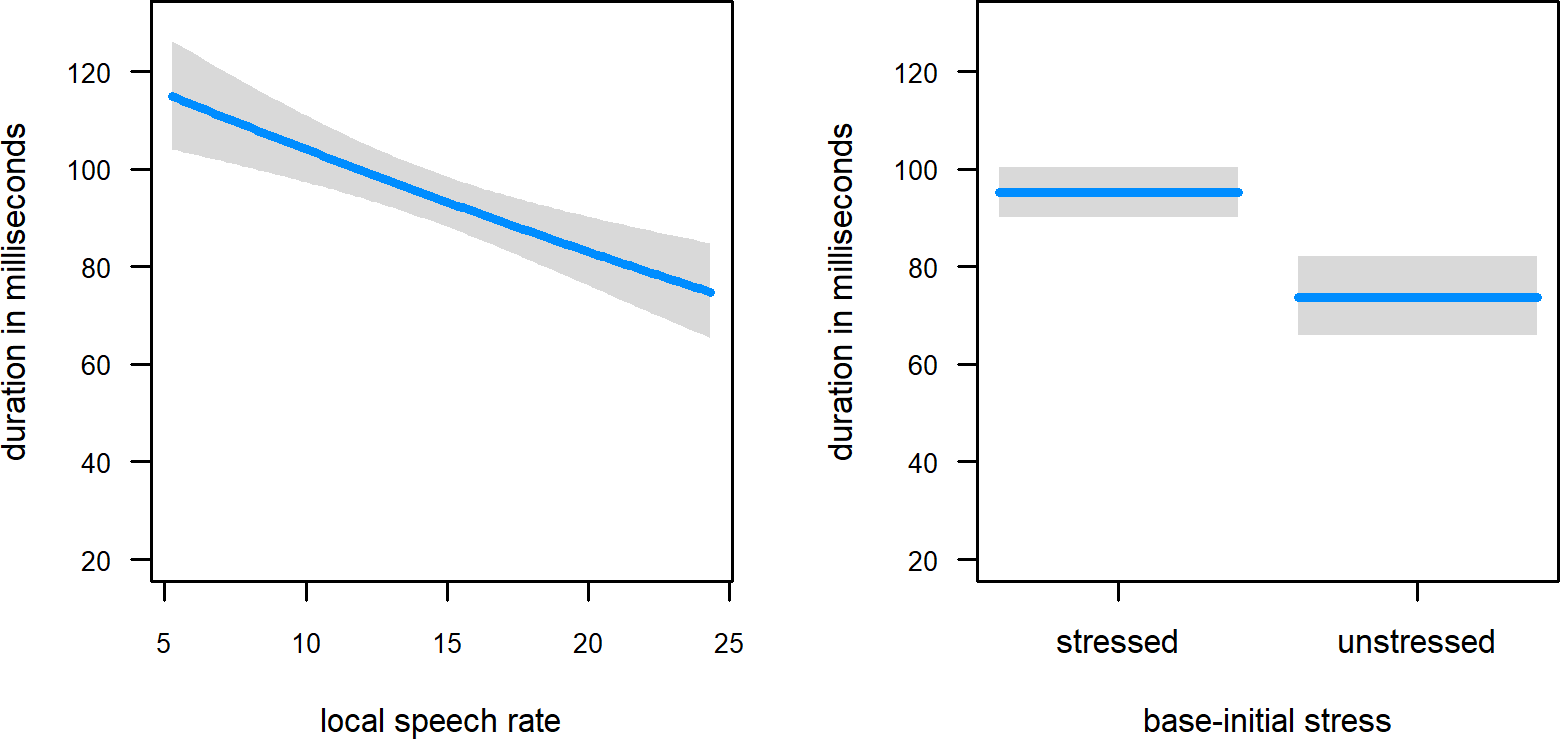
\includegraphics  [scale=0.8] {images/Corpus/inModelcov.png}
	\caption{Effects of local speech rate and base initial-stress on consonant duration in \prefix{in}data set}
	\label{fig:covariates in}
\end{figure*}

Let us turn to the variables of interest. The left panel of \figref{fig:inModel} displays the effect of \textsc{Environment}. Double consonants are significantly longer than singletons. The estimated mean duration for double consonants is 95~ms, while it is 68~ms for single consonants, a difference of 27~ms. This difference is significant, and shows that \prefix{in} geminates. 







\begin{figure*}
	
	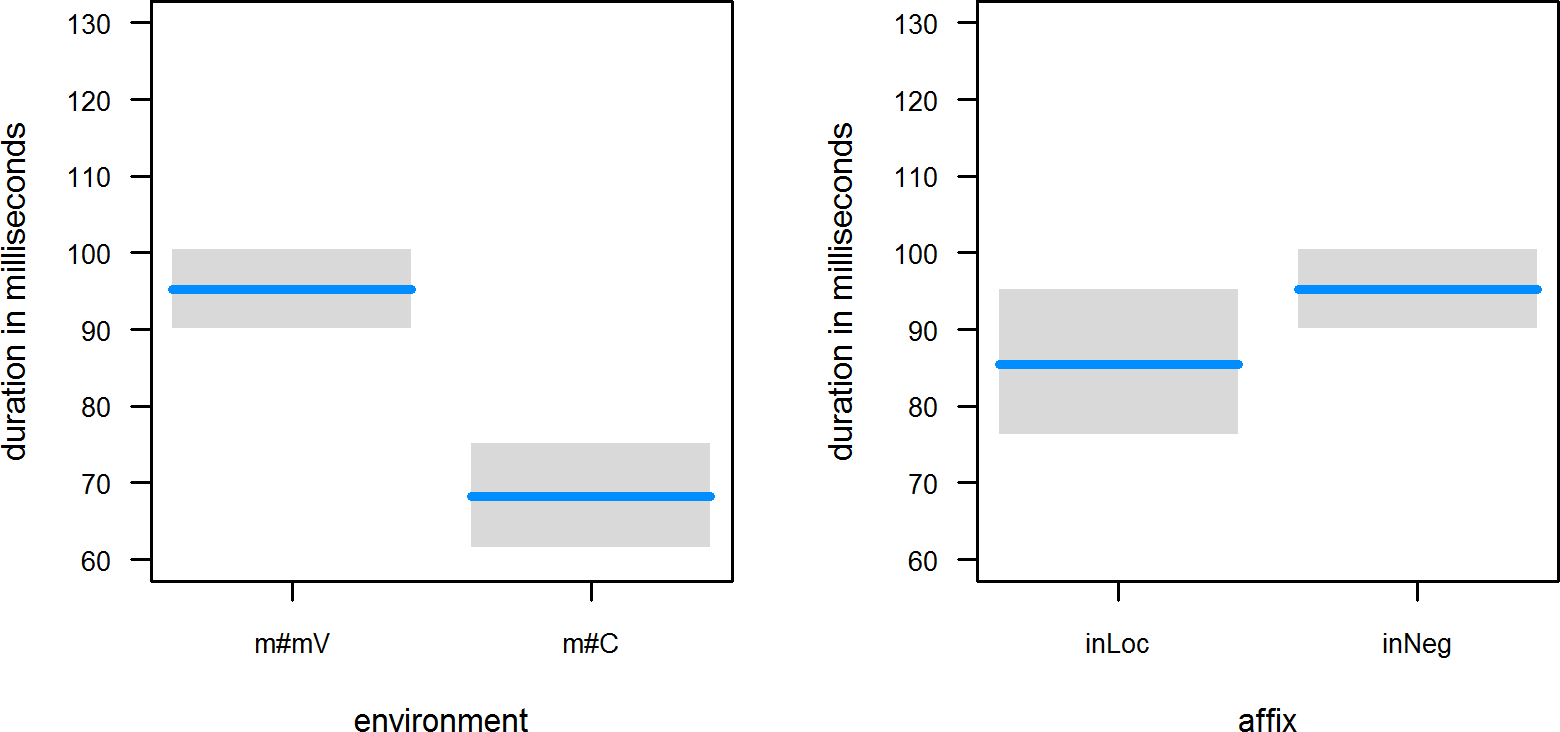
\includegraphics [scale=0.8]  {images/Corpus/inModel.png}
	\caption{Effects of environment and affix on consonant duration in \prefix{in}data set}
	\label{fig:inModel}
\end{figure*}



However, one could venture the idea that the difference is not due to a difference between one consonant and two, but due to a difference in the following segment, i.e. consonant versus vowel. This idea is, however, unsupported, since following vowels lead to shorter durations of the nasal. This can also be seen in the \prefix{un}data set, in which a single nasal preceding a consonant (63~ms) is longer than a single nasal preceding a vowel (43~ms). In other words, the double nasals (which are by their very nature followed by a vowel) are likely to be shortened, not lengthened, due to their vocalic environment. In other words, the double nasals show longer duration in spite of being in an environment that would trigger shorter duration. The significant difference between \texttt{m\#mV}  and \texttt{m\#C} is thus a sure sign of gemination.



The effect of \textsc{Affix} is displayed  in the right panel of \figref{fig:inModel}. The nasal in negative \prefix{in} is significantly longer (by 10~ms) than the one in locative \prefix{in}. Hence, there is a difference in the duration of the nasal depending on which of the two affixes is used. There was no interaction of \textsc{Environment} and \textsc{Affix}, which means that the two prefixes do not differ significantly in their gemination behavior.


None of the investigated decomposability measures proved to be significant. However, it is possible that, while the measures do not affect duration when tested individually, a combined measure of decomposability has a significant effect on consonant duration. As evidenced by the decomposability analyses in \sectref{corpus dec}, at least some of the decomposability variables highly correlate and can be assumed to measure the same underlying property. It is thus possible to test the effect of a combined measure of this underlying property. 

To test the effect of a combined decomposability measure, an additional model with combined decomposability measures (as opposed to individual decomposability measures) was fitted. The combined measures were created by means of a principal component analysis (cf. \sectref{stats} on principal component analyses). 
The principal component analysis was fitted with the variables log\textsc{Relative-Frequency}, \textsc{SemanticTransparency}, \textsc{SemanticTransparencyRating}, \textsc{TypeOfBase} and \textsc{Affix}. The variable \textsc{Affix} was included because of the differences in segmentability between locative and negative \prefix{in} (see \sectref{The decomposability of the four affixes: a comparison} for discussion). \textsc{LSAScore} was excluded because of the low number of observations coded for this variable. Categorical variables were recoded as numerical before entering the analysis, and all variables were scaled.
\tabref{tbl: summary PC in corpus} summarizes the analysis by showing the composition of each principal component, i.e. the loading of each variable for each principal component, and by displaying the proportion of variance covered by each component. 


\begin{table}
	\caption{ Summary of principal components}
	\label{tbl: summary PC in corpus}
	
			\resizebox{\textwidth}{!}{%		
		\begin{tabular}{lrrrrr}
			
			
			\lsptoprule
			
			
			\multicolumn{6}{l}{\textbf{Composition of principal components}}\\
			
			&PC1&          PC2 &       PC3       & PC4 & PC5  \\
			\midrule
			scaled\textsc{Affix }   &   0.078& -0.817 &-0.244 &0.449 & 0.255\\
			scaled\textsc{RelativeFrequency } &  -0.428& 0.450&-0.530 &0.574 & 0.054\\ 
			scaled\textsc{SemanticTransparencyRating}  &   -0.521&-0.233&  0.450& 0.269& -0.631\\
			scaled\textsc{TypeOfBase }&-0.487&-0.275 &-0.529&-0.623& -0.140\\
			scaled\textsc{SemanticTransparency }& -0.550& -0.002 & 0.420&-0.087&  0.717\\
			
			
			\midrule
			\multicolumn{6}{l}{\textbf{Variance explained by principal components}}\\
			&PC1&          PC2 &       PC3       & PC4 & PC5  \\
			\midrule
			Proportion of Variance &0.551& 0.264&  0.086& 0.064 &0.035\\
			\lspbottomrule                                                                                
		\end{tabular}
}
	


\end{table}



The analysis revealed that the first two components can account for most of the variance expressed by the five variables (81\%). An inspection of the rotation matrix shows that the first component is dominated by all four decomposability measures, and that the second is mainly dominated by the variable \textsc{Affix}. One can thus conclude that the first component represents a combined measure of decomposability, and the second represents the variable \textsc{Affix}. 
Both components were included as predictor variables in the linear model.  



The linear model with the principal components was fitted similarly to the model with the individual decomposability measures. After simplification, the model showed very similar effects as the model with the individual decomposability measures (see \hyperref[Appendix D: model summaries corpus]{appendix D} for model summary). The effects of \textsc{Environment}, \textsc{LocalSpeechRate} and \textsc{BaseInitialStress} are identical. Instead of the variable \textsc{Affix}, this model shows an effect of \textsc{PC2}. The effect is shown in \figref{fig:PC2 in Corpus}. The higher the value of \textsc{PC2}, the longer the duration of the nasal. As explained above, \textsc{PC2} is dominated by the variable \textsc{Affix}. A higher \textsc{PC2}-value indicates negative \prefix{in}, a lower \textsc{PC2}-value indicates locative \prefix{in}. On can thus interpret the effect of \textsc{PC2} as being an effect of \textsc{Affix}. Negative \prefix{in} is longer than locative \prefix{in}. The principal component model hence shows the same effects as the model with the individual decomposability measures.


\begin{figure*}
	
	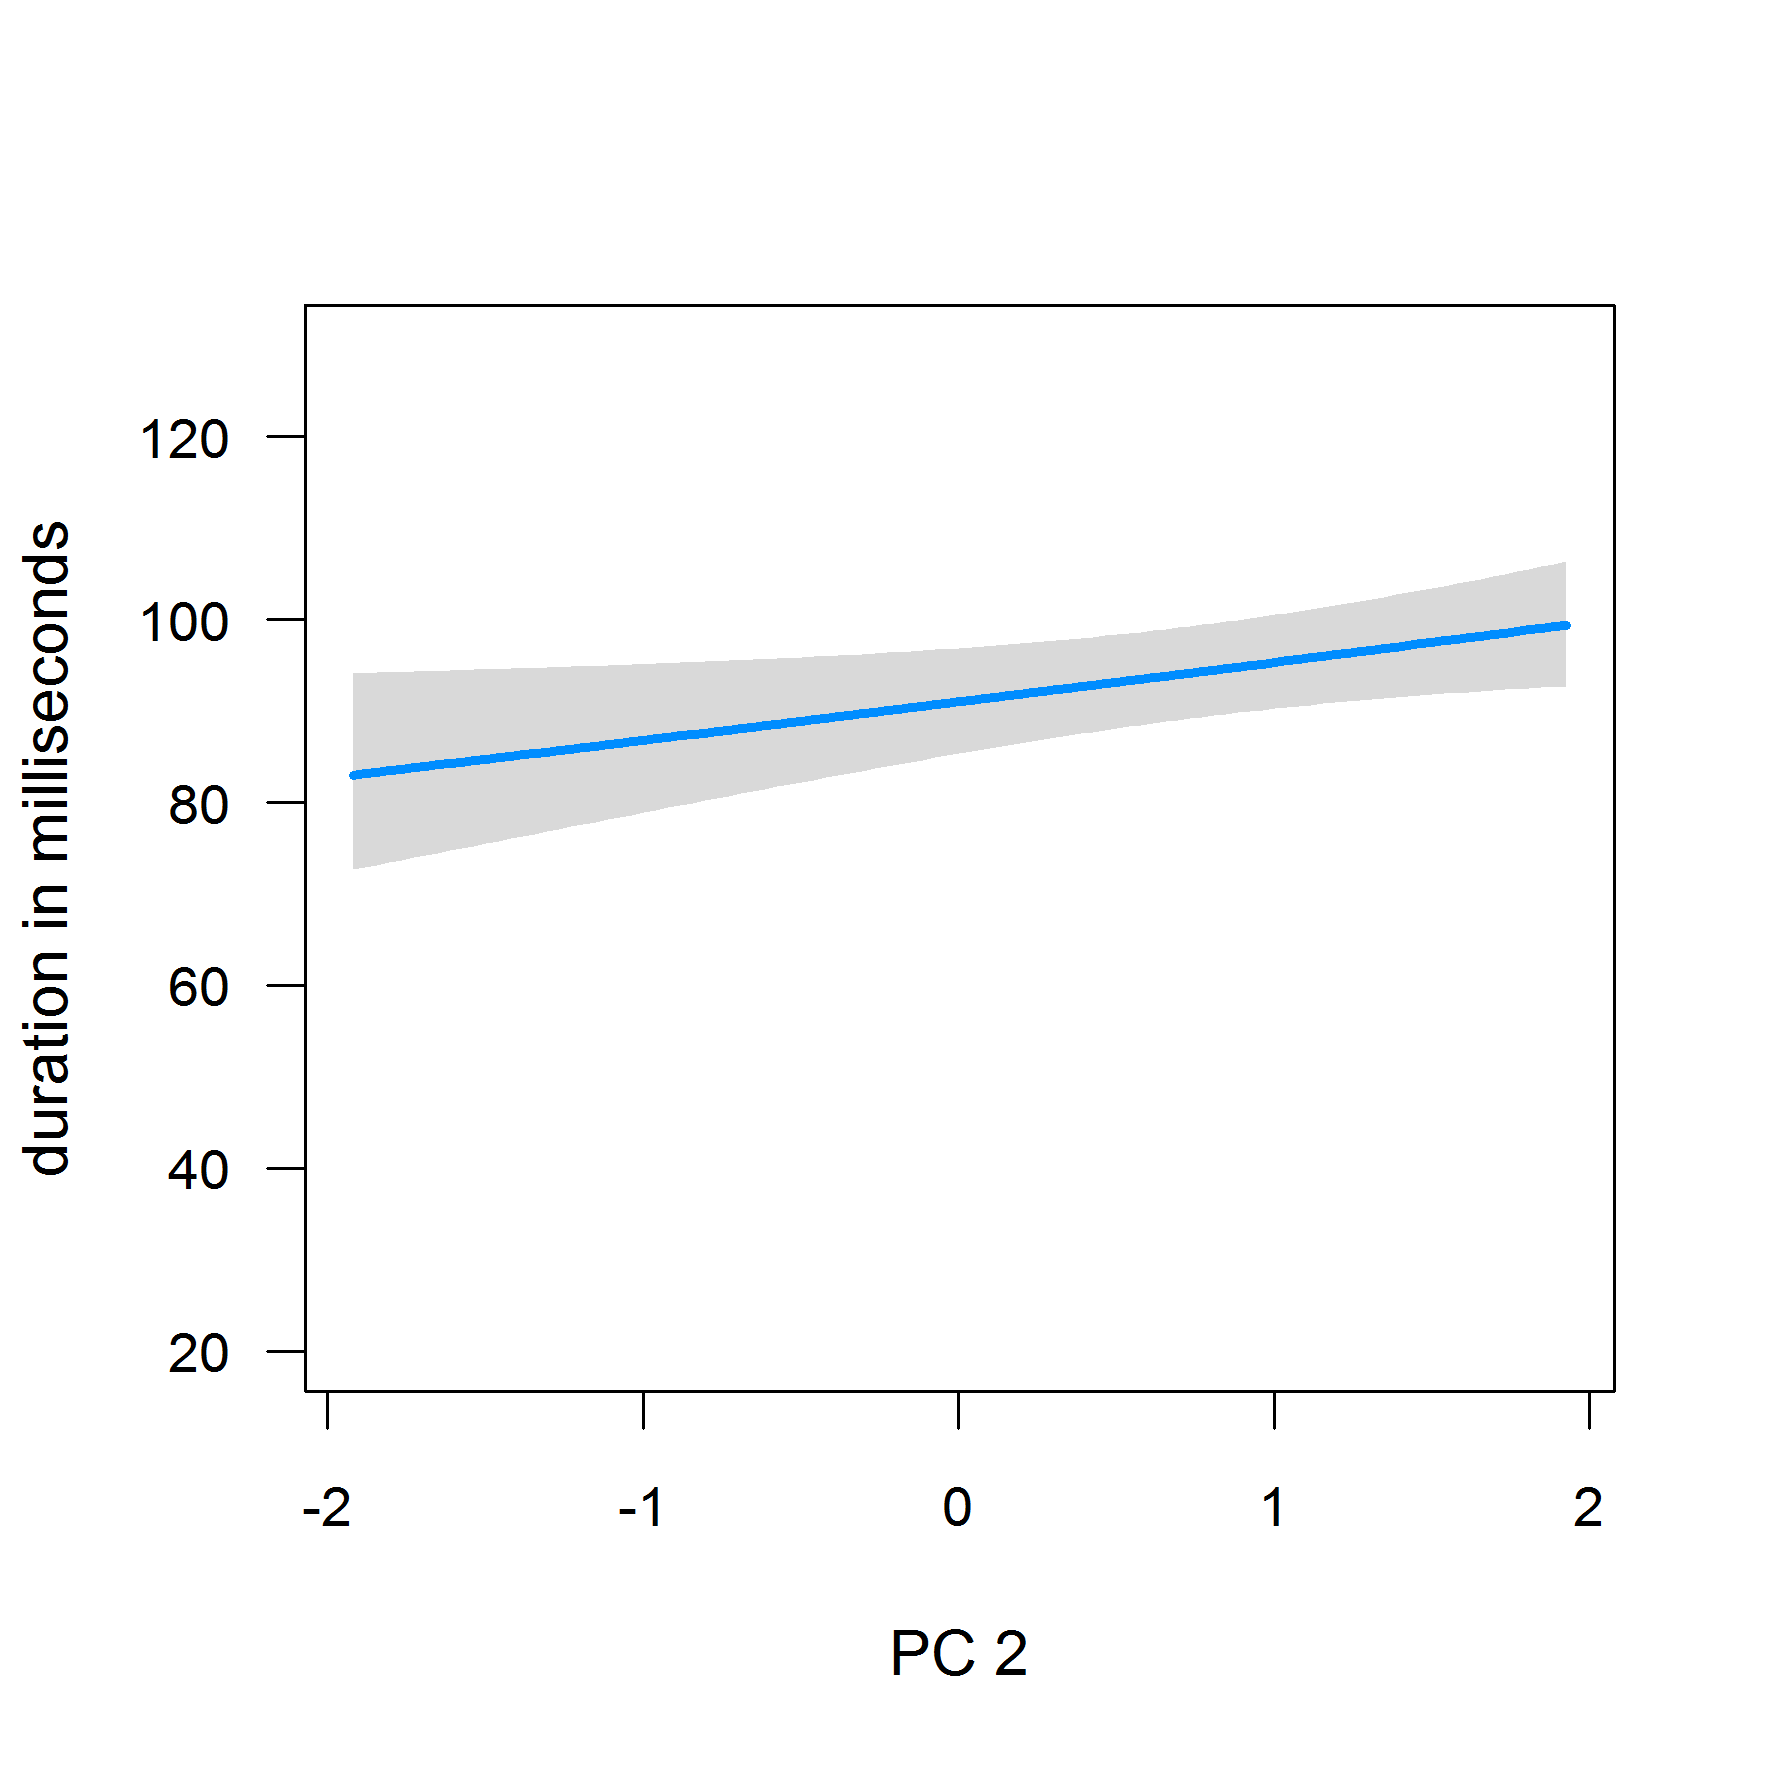
\includegraphics [scale=0.4] {images/Corpus/imPCAbsPC2.png}
	\caption{Effect of PC2 on consonant duration in \prefix{in}data set}
	\label{fig:PC2 in Corpus}
\end{figure*}



After the final models were fitted, multi-model inferencing  was used to detect the most important predictor variables. Due to the collinearity problems with the decomposability variables, these variables were not included separately in the analysis. Instead, the combined decomposability measure from the principal component analysis, i.e. principal component 1 (\textsc{PC1}), was included.
The analysis revealed that \textsc{LocalSpeechRate}, \textsc{Environment} and \textsc{BaseInitialStress} are the most predictive variables. They all have an importance value of $1$. \textsc{Affix} has an importance value of $0.79$, i.e. it is the fourth most important variable. With importance values of $0.29$ (\textsc{PC1}), $0.28$ (log\textsc{WordFormFrequency}) and $0.27$ (\textsc{PrecedingSegmentDuration}), the other variables are far less predictive of consonant duration. Multi-model-inferencing thus confirms the results of the final models.


\subsubsection{Relative duration}

In the model predicting relative consonant duration with \prefix{in}, the dependent variable was Box-Cox-transformed by the parameter $-0.101$ to achieve a normal distribution of the residuals. No outliers were excluded. The model was fitted similarly to the absolute duration model, i.e. the same interactions were tested and the decomposability measures were tested in the same way. On the one hand the decomposability variables were tested individually. On the other, decomposability was tested by means of principal components in an additional model. 

The simplification of both models, i.e. the one with the individual measures and the one with the principal components, resulted in same final model. The model features the three predictor variables \textsc{Environment}, \textsc{LocalSpeechRate} and \textsc{BaseInitialStress}. Neither the individual decomposability measures nor the principal components proved to be significant. There are no interactions. 
The summary of the final model is given in \tabref{tbl: summary model rel du in corpus}. The model explains about 42\% of the variance in the data.\\





\begin{table*}
	\caption{ Summary of linear model for variables predicting the Box-Cox-transformed relative duration of [m]  in \prefix{in}prefixed words}
	\label{tbl: summary model rel du in corpus}
	
			\resizebox{\textwidth}{!}{%		
		
		\begin{tabular}{lrrrr}
			
			
			\lsptoprule
			& Estimate & Std. Error & t-value & p-value  \\ 
			\midrule
			
			Intercept       & 0.987 & 0.015 & 65.285  &   	$< $0.001\\ 
			
			\textsc{Environment}-\texttt{m\#C } & 0.053 &   0.007 & 7.308 &$< $0.001\\ 
			
			
			\textsc{LocalSpeechRate}  				  &  -0.003 & 0.001 &  -3.416 & 0.001 \\ 
			
			\textsc{BaseInitialStress}-\texttt{unstressed}    & 0.066 &  0.008 & 7.876 & $< $0.001\\ 
			
			\midrule\\
			Adjusted R-squared: 0.422 \\
			\lspbottomrule
		\end{tabular}
}
	


\end{table*}


As in the model predicting absolute duration, this model reveals that double consonants are longer than singletons, i.e. we also find gemination in relative duration. Also similar to the absolute duration model, \textsc{LocalSpeechRate} affects consonant duration. The higher the speech rate, the shorter the nasal relative to the vowel. This effect of speech rate indicates that speech rate has a bigger effect on the consonant of the prefix \prefix{in} than on its vowel, i.e. in faster speech the consonant is more reduced than the vowel. A possible explanation might be that the prefixal vowel in \prefix{in} is too short to be reduced to the same degree as the prefixal nasal, i.e. there is simply less material to be reduced.

The model also reveals a significant effect of \textsc{BaseInitialStress}. In relative duration, the consonant is longer before unstressed syllables. This is the opposite of what is found for absolute duration, where the consonant is shorter in that condition. 
This difference between relative and absolute duration can be explained by the role of the preceding vowel for relative duration. Longer preceding vowels lead to shorter relative durations. One can thus assume that the shorter relative duration of the consonant in words with an unstressed base-initial syllable is caused by a longer preceding vowel in those words.
Longer vowels before unstressed syllables are expected. This is because, in the investigated words, unstressed base-initial syllables indicate a stressed prefix, which in turn might influence the duration of the prefixal vowel. It is particularly the duration of the vowel which is lengthened in a stressed syllable, i.e. one might expect the vowel of a stressed prefix (which is followed by an unstressed syllable) to be lengthened. A longer vowel in turn leads to shorter relative duration. This explains that in relative duration the consonant is shorter before unstressed base-initial syllables than before stressed base-initial syllables.
The absolute duration of the consonant, in contrast to its relative duration, is not affected by the duration of the preceding segment, i.e. by its stress status. Instead, the consonant participates in the stress-caused lengthening of its following syllable, i.e. the consonant is longer before stressed base-initial syllables. %The reverse effect of \textsc{BaseInitialStress} can thus be explained by the role of preceding vowel duration.

In contrast to the absolute model, in the relative duration model \textsc{Affix} does not have a significant effect. This indicates that negative and locative \prefix{in} only differ in absolute duration, i.e. the ratio of consonant and vowel duration does not differ between the two prefixes. 
As with absolute duration, no effect of the decomposability variables was found in the relative duration models. 

Multi-model inferencing revealed that the three variables which are significant in the final model are the most predictive variables across a multitude of models. \textsc{BaseInitialStress} has an importance value of $1$, \textsc{Environment}  has an importance value of $0.99$,  and  \textsc{LocalSpeechRate} has an importance value of $0.99$. The other tested variables are much less predictive of relative duration (importance value of log\textsc{WordFormFrequency}: $0.54$, importance value of \textsc{Affix}: $0.48$, importance value of \textsc{PC1}: $0.37$). 


\subsubsection{Summary}


The two linear models predicting consonant duration with \prefix{in} clearly show that locative and negative \prefix{in} geminate. In both models, phonological doubles are longer than phonological singletons. 
The absolute duration model furthermore revealed that the nasal in negative \prefix{in} is significantly longer than the one in locative \prefix{in}, irrespective of whether it is a double consonant or a singleton. This effect of \textsc{Affix} was, however, not found in relative duration.
With regard to the decomposability measure, none had an effect on nasal duration, neither in absolute, nor in relative duration. 
In both models, the two noise variables \textsc{LocalSpeechRate} and \textsc{BaseInitialStress} showed expected effects. None of the tested interactions was significant. 
The model predicting absolute consonant duration explains more of the variance in the data than the model predicting relative duration. 



\subsection{The Prefixes \prefix{un} and \prefix{in}} \label{corpus un in}


The model predicting consonant duration with \prefix{un} and \prefix{in} was fitted to directly compare the durational behavior of the nasals in the three prefixes \prefix{un}, negative \prefix{in} and locative \prefix{in}. The model has, however, the disadvantage that a number of interesting variables cannot be properly tested. The reason is that the \prefix{un} data set and the \prefix{in}data set differ in important respects.
First, the prefix \prefix{un} and the allomorph of \prefix{in} that is being invested here end in two different consonants, i.e.  /n/ vs. /m/. Therefore, durational differences between \prefix{un} and \prefix{in} are not directly comparable. I  used scaling of the durational variables to alleviate this problem. This, however, means that durational differences are not straightforward in their interpretation. 
Second, the phonological environments of singleton \prefix{un} and singleton \prefix{in} are not the same, since /ɪm/ is necessarily always followed by a base-initial consonant, while \prefix{un} is followed by both consonants and vowels. Only the double nasal in both prefixes is always followed by a vowel.
Third, variables of decomposability  cannot be tested in an interesting way. This is because \prefix{un}, as described in \sectref{The decomposability of the four affixes: a comparison}, does not vary in most of the decomposability measures, and because relative frequency measures are not well comparable across \prefix{un} and \prefix{in}. The prefix \prefix{in} has very many bound roots, which is problematic with regard to computing relative frequency measures that are comparable to the relative frequency measures of affixes with hardly any or no bound roots, i.e. in this case \prefix{un}. 
With these limitations in mind, a regression model was fitted to the lumped data set.  

Since the environments for the prefixal nasal are not the same across prefixes, I created a new variable in which I coded whether the word has one or two underlying nasals (\textsc{NumberOfConsonants}), and an additional variable encoding whether a vowel or a consonant followed the nasal (\textsc{FollowingSegment}). I included the following predictors in the model: \textsc{NumberOfConsonants}, \textsc{FollowingSegment}, \textsc{LocalSpeechRate},  \textsc{BaseInitialStress}, \textsc{Affix}, \textsc{PrecedingSegmentDuration} and log\textsc{WordFormFrequency}.
The model was then simplified and interactions were tested. Crucially, all interactions between the variable \textsc{Affix} and all other variables were tested (see \hyperref[Appendix C: Summaries of tested interactions in corpus study]{appendix C} for a list of all tested interactions). 
The final model explains 49\% of the variance and features five variables, \textsc{Number-OfConsonants}, \textsc{FollowingSegment}, \textsc{LocalSpeechRate}, \textsc{BaseInitialStress} and \textsc{Affix}. The model is documented in \tabref{tbl:corpus summary model un, in}.




\begin{table*}
	\caption{ Summary of linear model for variables predicting the normalized duration of the nasal in
		\prefix{un} and \prefix{in}prefixed words}
	\label{tbl:corpus summary model un, in}
	
		
			\resizebox{\textwidth}{!}{%				
		\begin{tabular}{lrrrr}
			
			
			\lsptoprule
			& Estimate & Std. Error & t-value & p-value  \\ 
			\midrule
			
			Intercept       & 2.484 &0.223  & 11.127  &   $<$ 0.001\\ 
			
			\textsc{NumberOfConsonants}-\texttt{double } & -1.454  &  0.144 & -10.065 & $<$ 0.001\\ 
			
			\textsc{FollowingSegment}-\texttt{vowel} & -0.537  & 0.130  & -4.136 & $<$ 0.001 \\ 			
			\textsc{LocalSpeechRate}  				  & -0.088 & 0.012 & -7.016 & $<$ 0.001\\ 
			
			\textsc{BaseInitialStress}-\texttt{unstressed}    & -0.347 &  0.103 & -3.365 & 0.001 \\ 
			
			\textsc{Affix}-\texttt{inLoc}   & -0.469  & 0.133 & -3.521 &   0.001\\ 
			\textsc{Affix}-\texttt{un}   & 0.343   & 0.123 & 2.794 &   0.006\\ 			
			\midrule\\
			Adjusted R-squared: 0.49  \\
			\lspbottomrule
		\end{tabular}
}
	
\end{table*}



\begin{figure*}
	
	
	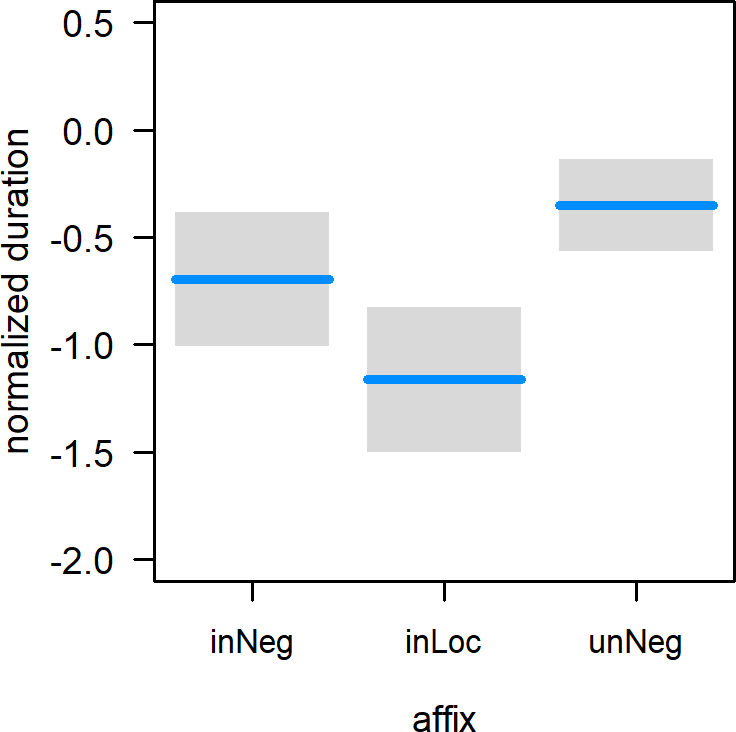
\includegraphics[scale=0.8] {images/Corpus/unInModel.png}
	\caption{Effects of  affix on consonant duration for words prefixed with \prefix{un} and \prefix{in}}
	\label{fig:inUnModel}
\end{figure*}



As in the \prefix{un} and \prefix{in}models, this model shows that doubles are longer than singletons. Interestingly, there is also  a  main effect of \textsc{Affix}. \figref{fig:inUnModel} shows that negative \prefix{in} is significantly longer than locative \prefix{in}, and that \prefix{un} is significantly longer than negative \prefix{in}.  We thus find a decline in duration from \prefix{un}, to negative \prefix{in}, to locative \prefix{in}. This decline is fully in line with the decline in segmentability of the prefixes found in \sectref{The decomposability of the four affixes: a comparison}. Crucially, there is no significant interaction between \textsc{Affix} and \textsc{NumberOfConsonants}, which means that all three prefixes geminate.

In addition to the effects of the variables of interest, there is the expected effect of \textsc{LocalSpeechRate} (nasals become shorter with increasing speech rate) and the expected effect of the \textsc{FollowingSegment} (nasals are shorter before vowels). There is also an effect of \textsc{BaseInitialStress} such that the nasal is shorter before unstressed syllables.

\subsection{The prefix \prefix{dis}} \label{corpus results dis}


\subsubsection{Absolute duration}

The residuals of the initial model predicting absolute consonant duration with \prefix{dis} were not distributed normally. Therefore, the dependent variable was Box-Cox-transformed (parameter:  $0.222$). After the model was refitted with the transformed dependent variable, it showed a satisfactory distribution of residuals. No outliers were removed. The model was then simplified according to the strategy described in \sectref{General Method}  and interactions were tested (see \hyperref[Appendix C: Summaries of tested interactions in corpus study]{appendix C} for a list of all tested interactions).

As in the \prefix{in}model, testing the effect of the decomposability measures simultaneously was not possible due to collinearity problems. Therefore, their effect was tested individually, as well as by using principal components. In other words, first models were fitted in which the effects of the decomposability measures were tested individually, and then an additional model with a combined decomposability measure was fitted. 
 Let us first discuss the model which initially included the individual measures.

An overview of the final model, i.e. the model after simplification, is given in \tabref{tbl: summary model4}. Insignificant estimates are printed in light gray. The model yields an adjusted R-squared of  0.333, i.e. it explains about 33\% of the variance found in the data. The model includes four variables, \textsc{Environment}, \textsc{LocalSpeechRate}, \textsc{Voicing} and \textsc{BaseInitialStress}. There is a significant interaction between \textsc{Environment} and \textsc{BaseInitialStress}. None of the decomposability variables is significant.


\begin{table*}
	\caption{ Summary of linear model for variables predicting the Box-Cox-transformed duration of [s] in \prefix{dis}prefixed words}
	\label{tbl: summary model4}
	
					\resizebox{\textwidth}{!}{%		
		\begin{tabular}{lrrrr}
			
			
			\lsptoprule
		 	                                     & Estimate & Std. Error & t-value & p-value  \\ 
			\midrule
			 Intercept                             & 0.644 &    0.015 & 43.659& $<$ 0.001\\	
					
			 \textsc{Environment}-\texttt{s\#C}  & -0.045 &    0.009 &  -5.176 & $<$ 0.001\\ 
			
			\textsc{Environment}-\texttt{s\#V}   & -0.026 &   0.010 & -2.506 & 0.014 \\ 
			
			\textsc{LocalSpeechRate}  				  &-0.005 & 0.001 & -4.595  &$<$ 0.001\\ 
			\textsc{Voicing}-\texttt{voiceless}   & 0.057 & 0.011 & 5.367 & $<$ 0.001\\ 		
			
			
			\textsc{BaseInitialStress}-\texttt{unstressed}   & -0.036 &  0.019 & -1.851 & 0.066 \\ 
			

			\textsc{Environment}-\texttt{s\#C}: &&&&\\
			\textsc{BaseInitialStress}-\texttt{unstressed}  & 0.048  &  0.023  & 2.068  & 0.041\\ 
			
			\textsc{Environment}-\texttt{s\#V}: &&&&\\
			\textsc{BaseInitialStress}-\texttt{unstressed}  & \color{lsLightGray}{0.017} & \color{lsLightGray} 0.021 &\color{lsLightGray}0.782  &\color{lsLightGray} 0.436 \\ 
			\midrule\\
			Adjusted R-squared: 0.333 \\
			\lspbottomrule
		\end{tabular}
}
	
\end{table*}






\begin{figure*}
	
	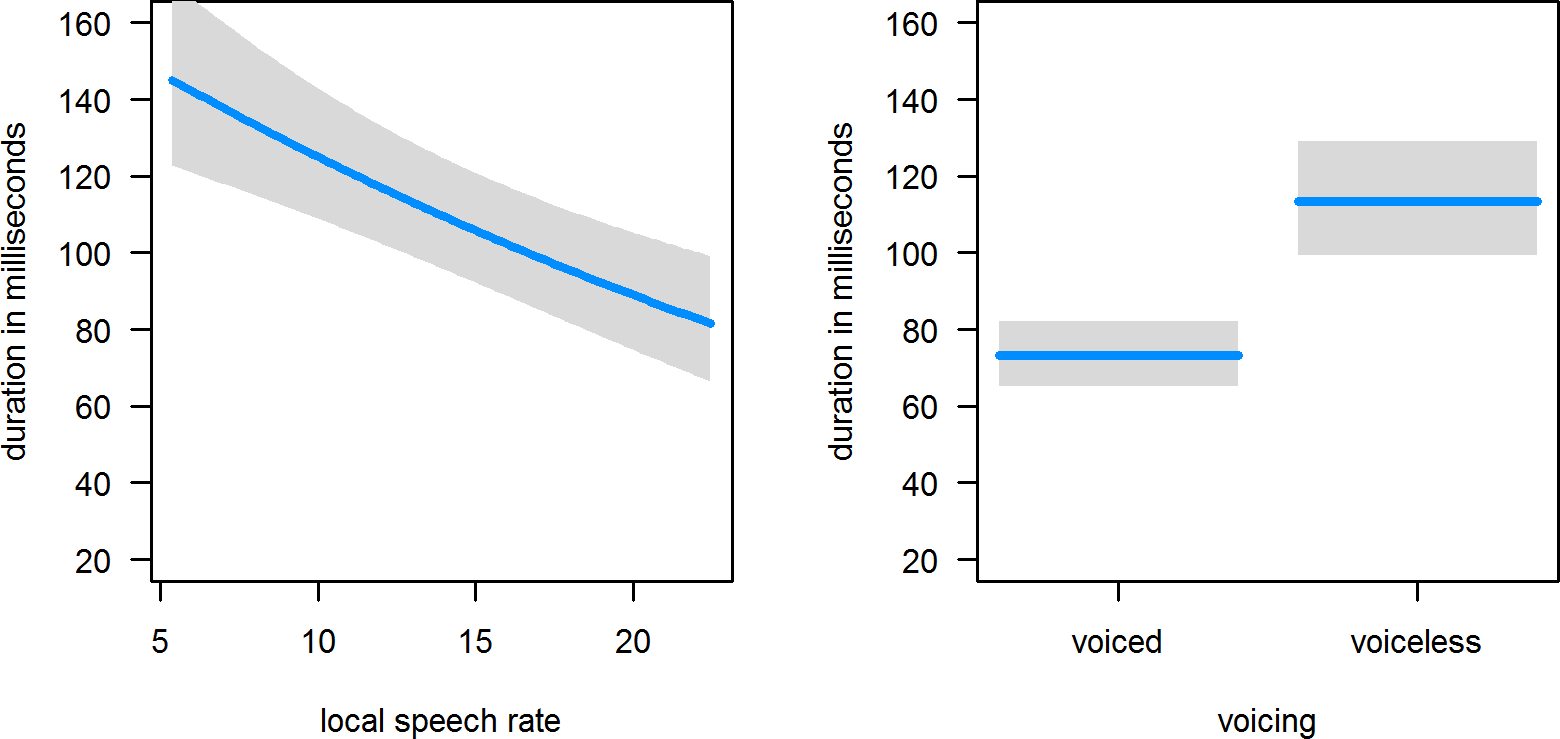
\includegraphics[scale=.8] {images/Corpus/disModelcov.png}
	\caption{ Effect of local speech rate and voicing on consonant duration in \prefix{dis}data set}
	\label{fig:corpus covariates dis}
\end{figure*}


%speech rate
\figref{fig:corpus covariates dis} displays the effects of \textsc{LocalSpeechRate} and \textsc{Voicing}. The effect of \textsc{LocalSpeechRate} can be seen in the left panel. As expected, with increasing speech rate the fricative in \prefix{dis}prefixed words becomes shorter. 
%voicing
The right panel of the figure shows the effect of \textsc{Voicing}. Voiced fricatives are significantly shorter than voiceless fricatives. For doubles this difference is predicted to be 47~ms, for singletons voiced fricatives are predicted to be 36~ms shorter than voiceless fricatives. 
With regard to \textsc{Voicing}, it is important to note that the distribution of voiced items in the data set is unbalanced. All voiced \prefix{dis}prefixed words are semantically opaque, followed by a vowel and have a stressed base-initial syllable. This skewed distribution might have influenced the final model, i.e. it might have skewed the effects of the affected variables. This problem will be discussed in further detail below.

\begin{figure*}

	
	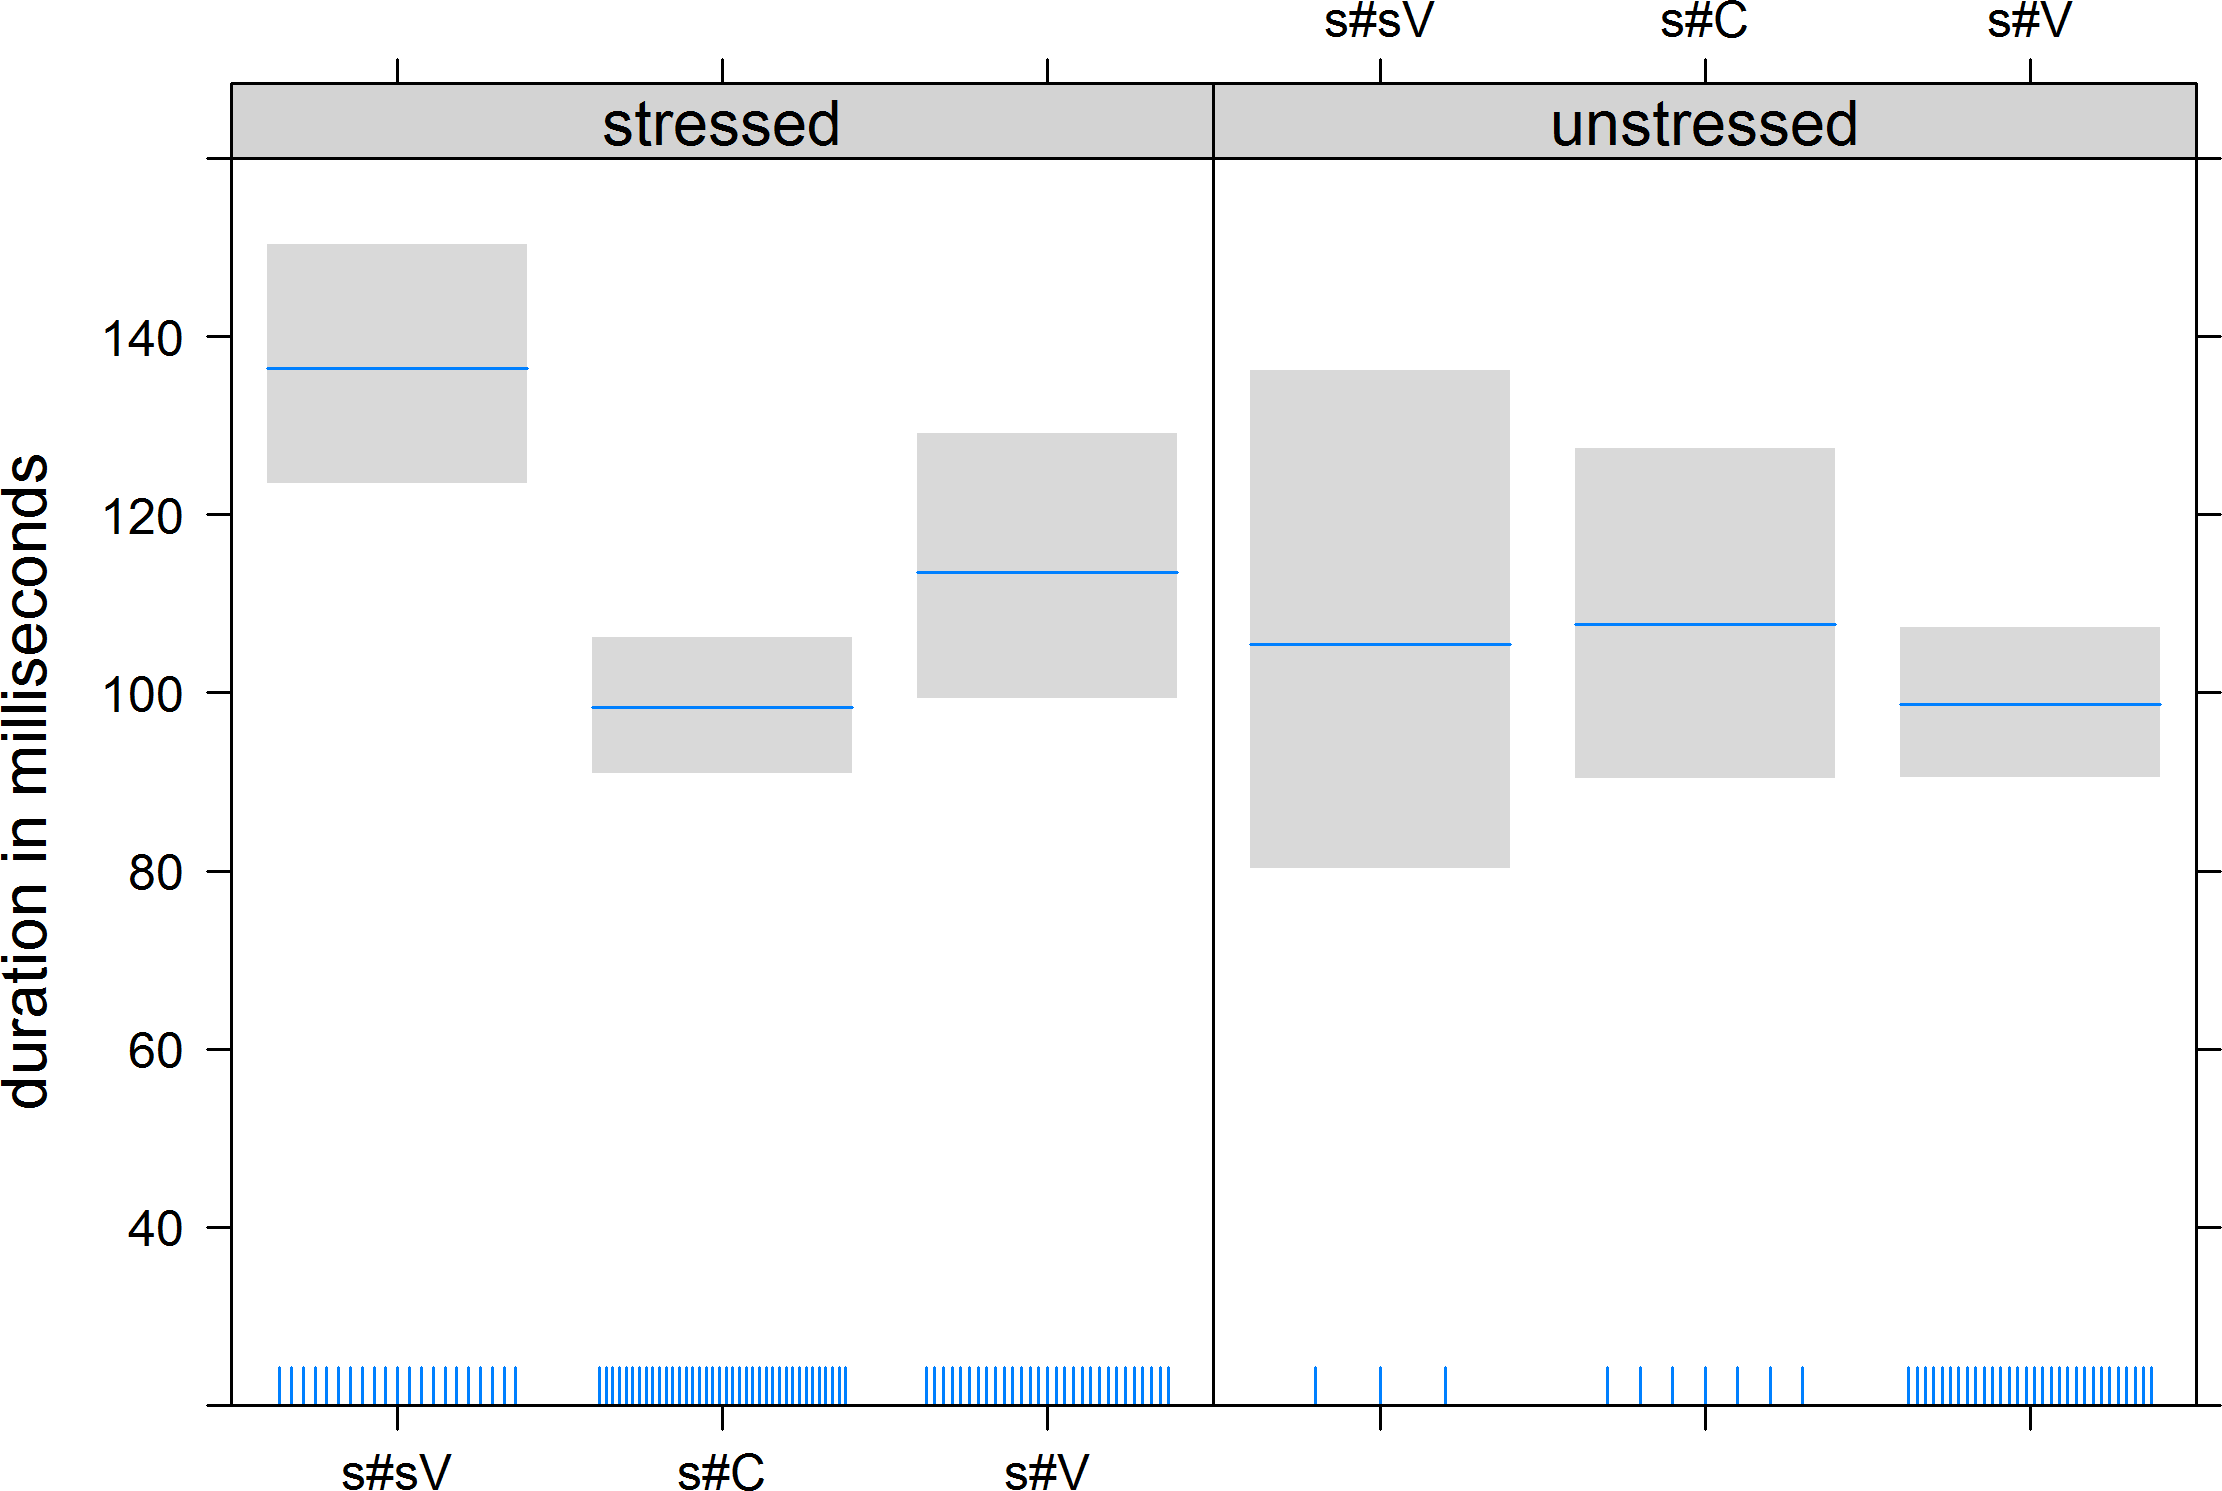
\includegraphics [scale=0.5]{images/Corpus/disModelTransitionTypeByStress.png}
	\caption{Effect of environment by base-initial stress on consonant duration in \prefix{dis}data set}
	\label{fig:corpus main effect 1 dis}
\end{figure*}

%Environment
The interaction between \textsc{Environment} and \textsc{BaseInitialStress} is displayed in \figref{fig:corpus main effect 1 dis}. The left panel of the figure displays the estimated effect of \textsc{Environment} on words with a stressed base-initial syllable. The right panel shows the estimated effect of \textsc{Environment} on words with an unstressed base-initial syllable. The figure shows that while there is a significant effect of \textsc{Environment} for words with a stressed base-initial syllable, there is no significant effect for words with an unstressed base-initial syllable. For words with a stressed base-initial syllable, doubles are estimated to be 38 ms  longer than singletons which are followed by a consonant, and 23 ms longer than singletons which are followed by a vowel. 
The difference in duration between the two singleton levels is marginally significant (p-value: $0.066$). The fricative before a consonant is predicted to be 15ms shorter than the fricative before a vowel.  There is no difference between the three environments for words with an unstressed base-initial syllable, i.e. doubles are of the same duration as singletons, and the two singleton levels are  also of the same duration. 


%



One could interpret the interaction between \textsc{Environment} and \textsc{BaseInitialStress} as evidence that the prefix \prefix{dis} only geminates when followed by a stressed syllable, and that only in this condition the following segment, i.e. consonant or vowel, affects the duration of the prefixal consonant. However, there are two problems with the pertinent interaction, and the interpretation of the effects is therefore not that straightforward. Both problems are related to the distribution of variables in the data set. 

%first problem
The first problem is the number of types and tokens for each category. The blue lines on the bottom of the plot (in \figref{fig:corpus main effect 1 dis}), the rugs, indicate the number of tokens for each category. It is striking that there are only three tokens with an unstressed base-initial syllable and a double consonant at the morphological boundary. These three tokens are all of the same type, i.e. \textit{dissolution}. The interaction found in the model is hence caused by only three observations (of one type). In other words, there are only three tokens with a double consonant which do not geminate. All three tokens are of the type \textit{dissolution}. 

One might argue that the word \textit{dissolution} behaves differently because the word is simplex. There are two arguments for this assumption. First, \prefix{dis} does not carry any meaning in the word \textit{dissolution}. Second, in the morphologically related derivative \textit{dissolve} the prefixal fricative is voiced. As discussed in \sectref{description un}, there are claims that voiced /s/ is only found in simplex \prefix{dis}words. That the word \textit{dissolve} features a voiced fricative might thus indicate that it is lexicalized, which in turn might also mean that the related word \textit{dissolution} is lexicalized and no longer complex.

The second problem with the interaction  
is related to the distribution of the variable \textsc{Voicing}. 
 As already mentioned above, all voiced \prefix{dis}prefixed words are semantically opaque, followed by a vowel and have a stressed base-initial syllable. The significant effect of \textsc{Voicing} in the final model is thus solely based on opaque, vowel-adjacent items with stressed base-initial syllables. Even though the effect is based on only a few items with a particular combination of features, the model accounts for \textsc{Voicing} in predicting consonant duration for all items of all levels. In other words, the model allocates the effect of \textsc{Voicing} to all levels irrespective of whether voiced items are actually present in the pertinent level. This might distort the effects of the affected variables, i.e. \textsc{SemanticTransparency}, \textsc{Environment} and \textsc{BaseInitialStress}. 
  With regard to the final model, the interaction between \textsc{Environment} and \textsc{BaseInitialStress} might be affected by this problem.
  Only two of the six pertinent categories feature voiced items, i.e. only words with base-initial stress and a double consonant and words with base-initial stress and a singleton followed by a vowel can be voiced. All other categories only feature voiceless items.
  
  
  
  To test whether the effects of \textsc{Environment} and \textsc{BaseInitialSyllable} are affected by the distribution of voiced items in the data set, and to also test the effect of \textsc{SemanticTransparency} without the possible harming influence of the variable \textsc{Voicing}, an additional model was fitted to the \prefix{dis}data set. In this model only voiceless \prefix{dis}prefixed words were included. The model included 104 observations, i.e. 24 voiced \prefix{dis}prefixed words were excluded. 
  
  


 
\begin{table*}
	\caption{ Summary of linear model for variables predicting the Box-Cox-transformed duration of [s] in \prefix{dis}prefixed words with voiceless /s/}
	\label{tbl: summary model6}
	
					\resizebox{\textwidth}{!}{%		
		\begin{tabular}{lrrrr}
			
			
			\lsptoprule
			& Estimate & Std. Error & t-value & p-value  \\ 
			\midrule
			Intercept                             &0.716 &    0.017 &41.928 & $<$ 0.001\\	
			
			\textsc{Environment}-\texttt{s\#C}  &-0.050 &     0.009 &  -5.607 &$<$ 0.001\\ 
			
			\textsc{Environment}-\texttt{s\#V}   & -0.052 &   0.011 & -4.918 &$<$ 0.001 \\ 
			
			\textsc{SemanticTransparency}-\texttt{transparent}  &
			\color{lsLightGray}{-0.004 }& \color{lsLightGray} 0.008 & \color{lsLightGray}-0.523   &  \color{lsLightGray}0.602  \\ 
			
			\textsc{SpeechRate}  				  &-0.005 & 0.001 & -5.088   &$<$ 0.001 \\ 
			
			\textsc{BaseInitialStress}-\texttt{unstressed}   & -0.046 &   0.017 & -2.748 & 0.007 \\ 
			

			\textsc{SemanticTransparency}-\texttt{transparent}: &&&&\\
			\textsc{BaseInitialStress} - \texttt{unstressed}  & 0.052 &  0.020 & 2.646 & 0.010\\ 
			\midrule\\
			Adjusted R-squared: 0.375\\
			\lspbottomrule
		\end{tabular}
}
	
\end{table*}

The model predicting consonant duration with voiceless \prefix{dis}prefixed words was fitted similarly to the model with all items. 
\tabref{tbl: summary model6} shows the final model for the voiceless fricatives. It explains about 38\% of the variance found in the data. 
As in the model with all \prefix{dis}prefixed words, \textsc{LocalSpeechRate} has the expected effect on duration, and we find an effect of \textsc{BaseInitialStress} and \textsc{Environment}. However, in contrast to the complete model, in this model \textsc{BaseInitialStress} and \textsc{Environment} are not interacting. 
\figref{fig:corpus main effect 1 dis without voiced items} shows the effect of  \textsc{Environment}. One clearly sees that the double is predicted to be longer than both singleton consonants, irrespective of base-initial stress. Furthermore, the durational difference between the two singleton levels is not significant in this model. One can hence assume that the marginally significant difference between the two singleton levels in the complete model was caused by the uneven distribution of voiced items in the complete \prefix{dis}data set. 


\begin{figure*}
	
	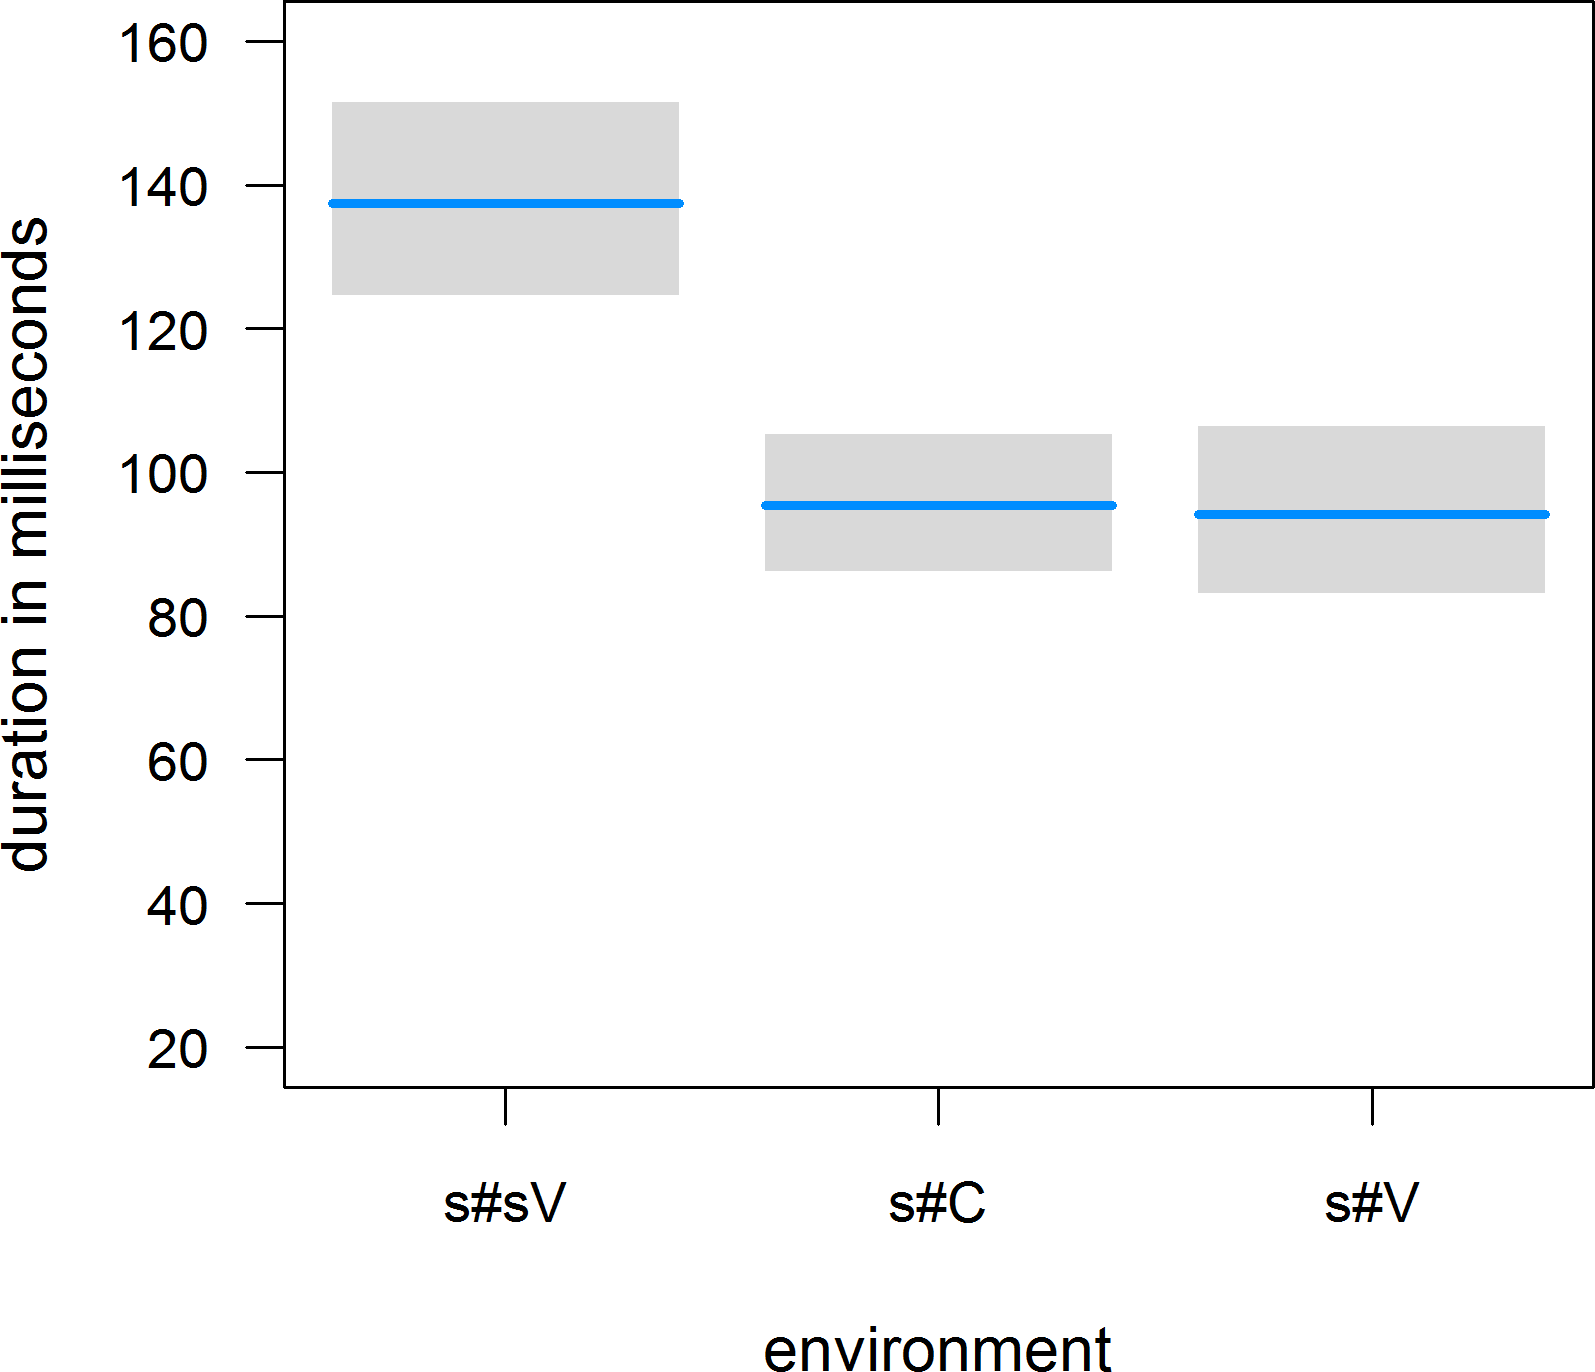
\includegraphics [scale=0.4]{images/Corpus/disModelWithoutVoicedSoundsEnvironment.png}
	\caption{ Effects of environment on consonant duration in voiceless \prefix{dis}data set}
	\label{fig:corpus main effect 1 dis without voiced items} 
\end{figure*}


\begin{figure*}
	

	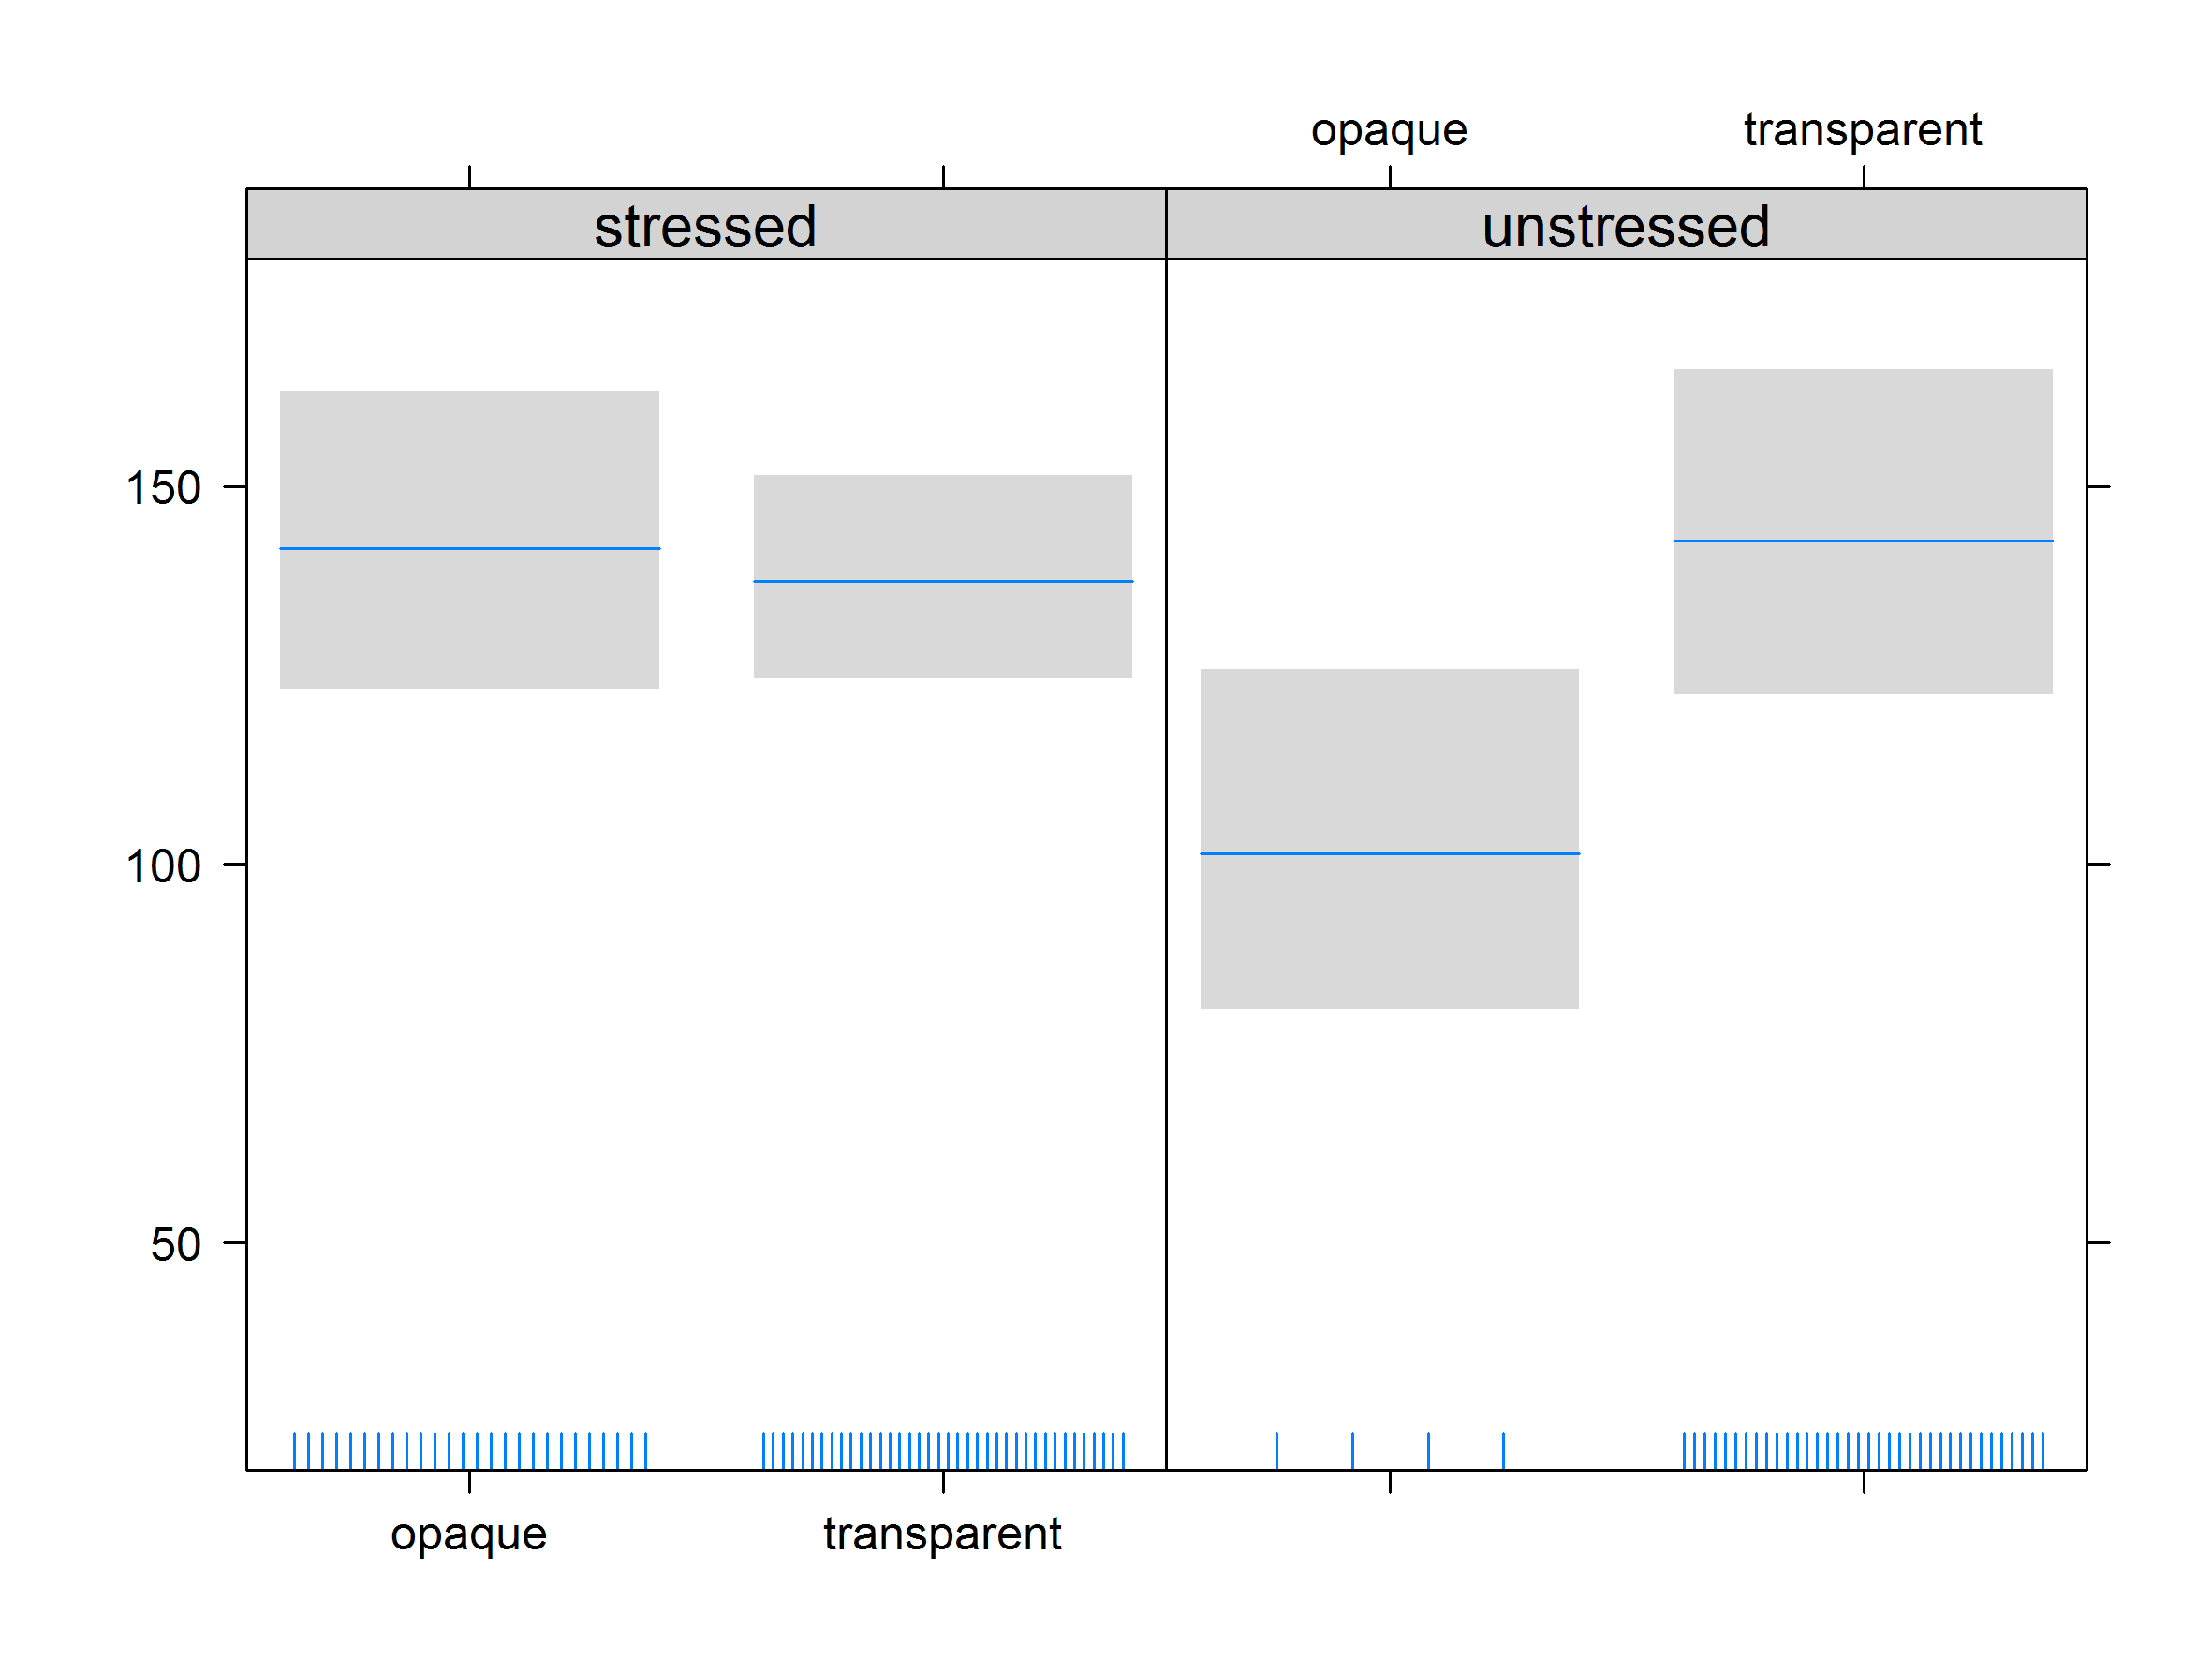
\includegraphics [scale=0.5]{images/Corpus/disModelWithoutVoicedSoundsSemanticTransTypeByStress.png}
	\caption{Effects of semantic transparency by  base-initial stress on consonant duration in voiceless \prefix{dis}data set}
	\label{fig:corpus main effect 2 dis without voiced items}
\end{figure*}






The voiceless model shows an interaction between the two variables \textsc{Semantic-Transparency} and \textsc{BaseInitialStress}. This interaction can be seen in \figref{fig:corpus main effect 2 dis without voiced items}. The left panel shows the effect of \textsc{SemanticTransparency} for items with a stressed base-initial syllable, the right panel shows the effect for items with an unstressed base-initial syllable. When the base-initial syllable is stressed, there is no difference between opaque and transparent items. When the base-initial syllable is unstressed, the fricative in opaque items is predicted to be 42 ms shorter than the fricative in transparent items. However, as in the complete model one must be cautious to  interpret this interaction. There are only four opaque tokens with an unstressed base-initial syllable in the data set. These four tokens cause the interaction, i.e. in these four tokens the fricative is significantly shorter than in all other tokens. 
Crucially, three of the four tokens are of the type \textit{dissolution}. This means that, even though we find two different interactions in the two \prefix{dis}models (\textsc{BaseInitialStress} and \textsc{Environment} in the complete model vs. \textsc{BaseInitialStress} and \textsc{SemanticTransparency} in the voiceless model), the same tokens which cause the interaction in the complete model cause the interaction in the model with only voiceless items. It remains unclear whether the short fricative in the pertinent words is due to the unstressed base-initial syllable in combination with semantic opacity, or whether the pertinent words behave differently because the stress status of the base-initial syllable is crucial for gemination with \prefix{dis}, i.e. only words with a stressed base-initial syllable geminate, or whether the shorter fricative duration is caused by type-specific effects. 



After fitting a model with the individual decomposability measures, I fitted a model with combined decomposability measures. The combined measures were created by means of a principal component analysis (cf. \sectref{stats} on principal component analyses). 
The principal component analysis included the four variables log\textsc{RelativeFrequency}, \textsc{SemanticTransparencyRating}, \textsc{TypeOfBase} and \textsc{SemanticTransparency}. As with \prefix{in}, the variable \textsc{LSAScore} was not included in the principal component analysis as it would have led to an extreme reduction of the data set. Categorical variables were recoded as numerical before they entered the analysis, and all variables were scaled.




\tabref{tbl: summary PC discorpus} shows a summary of the principal components. The first principal component accounts for most of the variance and is composed more or less equally of all measures. The second component is dominated by \textsc{TypeOfBase} and log\textsc{RelativeFrequency}, the third component mostly represents \textsc{SemanticTransparency}, \textsc{TypeOfBase} and log\textsc{RelativeFrequency}, and the fourth is mostly composed of \textsc{SemanticTransparency} and \textsc{SemanticTransparencyRating}. The second and the third component explain much less variance than the first, and the last principal component explains barely any variance. The first three principal components were included in the model.



After model simplification none of the principal components remained in the model. The final model resembles the final model of the complete data set. This means that the four variables \textsc{Environment}, \textsc{LocalSpeechRate}, \textsc{Voicing} and \textsc{BaseInitialStress} proved to be significant, and that \textsc{Environment} and \textsc{BaseInitialStress} form an interaction in the model. Decomposability did not affect fricative duration. 


\begin{table*}
	\caption{ Summary of principal components}
	\label{tbl: summary PC discorpus}
	
		\resizebox{\textwidth}{!}{%		
			\begin{tabular}{lrrrr}
				
				
				\lsptoprule
				
				
				\multicolumn{5}{l}{\textbf{Composition of principal components}}\\
				
				&PC1&          PC2 &       PC3       & PC4   \\
				\midrule
				
				scaled\textsc{RelativeFrequency } &  0.449&  0.653 & 0.609& 0.036\\ 
				scaled\textsc{SemanticTransparencyRating}  &   0.563 &-0.094 &-0.269& -0.776\\
				scaled\textsc{TypeOfBase }&0.441& -0.735 & 0.447  & 0.255\\
				scaled\textsc{SemanticTransparency }& 0.535  &0.158 &-0.598 &  0.576\\
				\midrule
				\multicolumn{5}{l}{\textbf{Variance explained by principal components}}\\
				&PC1&          PC2 &       PC3       & PC4  \\
				\midrule
				Proportion of Variance &0.679& 0.174& 0.105& 0.042\\
				\lspbottomrule
			\end{tabular}
		}
	
\end{table*}

%Mumin voiced
Two multi-model inferencing analyses were conducted for \prefix{dis}, one for the complete data set, one for the voiceless data set. As with \prefix{in}, the principal components were used to test the predictive value of the decomposability variables. In other words, to avoid collinearity problems, the principal components were used in the analyses instead of the individual decomposability measures. 

The models revealed that \textsc{LocalSpeechRate} and \textsc{Environment}  are the most important variables in both models (importance value: $1$). In the complete model, \textsc{Voicing} was also of high importance (importance value: $1$). 
For both data sets, \textsc{BaseInitialStress} proved to be the next most important variable. However, its importance value is much lower than the ones of \textsc{Environment}, \textsc{LocalSpeechRate} and \textsc{Voicing} ($0.47$ in complete model, $0.32$ in voiceless model).
 All other variables were much less important in both models. 
The importance values for the complete model are $0.37$ for log\textsc{WordFormFrequency},  $0.26$ for \textsc{PrecedingSegmentDuration}, $0.29$ for \textsc{PC2}, $0.25$ for \textsc{PC1},  and $0.25$ for \textsc{PC3}; 
 the importance values for the voiceless model are $0.30$ for \textsc{PC3}, $0.28$ for log\textsc{WordForm-Frequency}, $0.28$ for \textsc{PC1}, $0.27$ for \textsc{PC2} and $0.30$ for \textsc{PrecedingSegmentDuration}.



\subsubsection{Relative duration}

In the model predicting relative duration with \prefix{dis}, the residuals showed a normal distribution and therefore no transformation of the dependent variable was necessary. The model was fitted similarly to the absolute duration model, i.e. decomposability measures were tested individually, as well as in terms of principal components, and the same interactions were tested. Let us first discuss the model with the individual decomposability measures.

After model simplification, the following four variables remained in the final model: \textsc{Environment}, \textsc{SemanticTransparency}, \textsc{Voicing} and \textsc{BaseInitialStress}. With an adjusted R-squared of $0.262$ the model explains less of the variance than the absolute duration model. The model summary is printed in \tabref{tbl: summary model5}.
  
    \begin{table*}
    	\caption{ Summary of linear model for variables predicting the relative  duration of [s] in \prefix{dis}prefixed words}
    	\label{tbl: summary model5}
    	
    					\resizebox{\textwidth}{!}{%		
    		\begin{tabular}{lrrrr}
    			\lsptoprule
    			& Estimate & Std. Error & t-value & p-value  \\ 
    			\midrule
    			Intercept                             & 1.937 &   0.231  & 8.384 &$<$ 0.001\\	
    			
    			\textsc{Environment}-\texttt{s\#C}  & -0.838  &   0.203 &-4.134  &$<$ 0.001\\ 
    			
    			\textsc{Environment}-\texttt{s\#V}   &-0.643 & 0.208 &-3.089 & 0.002\\ 
    			
    			\textsc{SemanticTransparency}-\texttt{transparent}				   & -0.390 &   0.194 &-2.015 &0.046\\ 
					
    			\textsc{Voicing}-\texttt{voiceless}   &1.187 &0.281 &  4.225  & $<$ 0.001 \\ 	
    			
    			
    			\textsc{BaseInitialStress}-\texttt{unstressed}   &-0.370 &  0.185  & -1.998  &0.048 \\ 

    			\midrule\\
    			Adjusted R-squared: 0.262\\
			\lspbottomrule
    		\end{tabular}
    	}
    	
    \end{table*}
  
The variable \textsc{Voicing} shows the same effect as in the absolute duration model. Voiced fricatives are shorter than voiceless fricatives.
The effects of \textsc{Environment} and \textsc{BaseInitialStress} are also similar to the ones found in the absolute duration model. Doubles are longer than singletons, and consonants are shorter before unstressed base-initial syllables than before stressed base-initial syllables. 
In contrast to the absolute duration model, the relative duration model does not show an interaction between \textsc{Environment} and \textsc{BaseInitialStress}, or between \textsc{SemanticTransparency} and \textsc{BaseInitialStress}. This means that, in contrast to the absolute duration model,  all \prefix{dis}prefixed types geminate in terms of their relative duration. Furthermore, all prefixal fricatives are affected by an unstressed base-initial syllable, i.e. not just opaque words or words with a double consonant.

The effect of \textsc{BaseInitialStress} on relative duration with \prefix{dis} deviates from the effect of \textsc{BaseInitialStress} on relative duration with \prefix{in}. For \prefix{in}, we find shorter relative durations before stressed syllables than before unstressed syllables. This effect was explained by reference to the preceding vowel duration in \prefix{in}. There are different possibilities for the deviating results between \prefix{in} and \prefix{dis}. It might for example be that inherent durational differences between the consonants, i.e. /m/ vs. /s/, led to different results. Another possibility is that preceding vowel durations differ between \prefix{in} and \prefix{dis}.
          

 The final relative duration model shows a significant effect of \textsc{SemanticTrans-parency}. Transparent items are predicted to have shorter fricatives than opaque items. This is an unexpected effect, which is not found in absolute duration, and one must be cautious to interpret the effect. 
 As discussed above, there is a close and complex relation between the variables \textsc{Voicing} and \textsc{SemanticTransparency}. This relation might have caused the surprising result. To see whether this is the case, an additional model with only voiceless items was fitted. The model is displayed in \tabref{tbl: summary model7}.
 With an R-squared of $0.204$, the model explains 20\% of the data. This is less than any other model fitted to the \prefix{dis}data set. Only one variable remained significant in the model, \textsc{Environment}. The fricative in \texttt{s\#sV}-structures is longer than the fricative in \texttt{s\#C}- and \texttt{s\#V}-structures. In other words, the model again shows that \prefix{dis} geminates. 
 Crucially, \textsc{SemanticTransparency} does not reach significance in the model. One can therefore conclude that the effect found in the complete model is probably caused by the distribution of voicing in the data set. In other words, the effect is not stable and therefore not trustworthy.

    \begin{table}
    	\caption{ Summary of linear model for variables predicting the relative  duration of [s] in \prefix{dis}prefixed words with voiceless /s/}
    	\label{tbl: summary model7}
    	
    					\resizebox{\textwidth}{!}{%		
    		\begin{tabular}{lrrrr}
    			\lsptoprule
    			& Estimate & Std. Error & t-value & p-value  \\ 
    			\midrule
    			Intercept                             & 2.878   &  0.172 & 16.692  & $<$ 0.001 \\	
    			
    			\textsc{Environment}-\texttt{s\#C}  & -0.823 &  0.207&  -3.970 &  $<$ 0.001\\ 
    			
    			\textsc{Environment}-\texttt{s\#V}   &-1.123  &   0.212&  -5.295 &$<$ 0.001 \\
    			
    			
    			\midrule\\
    			Adjusted R-squared: 0.204 \\
			\lspbottomrule
    		\end{tabular}
    	}
    	
    \end{table}



After fitting the model with the individual decomposability measures, the model with the principal components was fitted. After simplification, the principal component model showed similar effects as the model with the individual decomposability measures (see \tabref{model im PC Corpus abs} in \hyperref[Appendix D: model summaries corpus]{appendix D} for model summary). The effects of \textsc{Environment} and \textsc{Voicing} are identical. However, instead of the variables \textsc{BaseInitialStress} and \textsc{SemanticTransparency}, this model includes the variable \textsc{PC1}. 
The effect of \textsc{PC1} is shown in \figref{fig:PC1 dis Corpus}. 


\begin{figure*}
	
	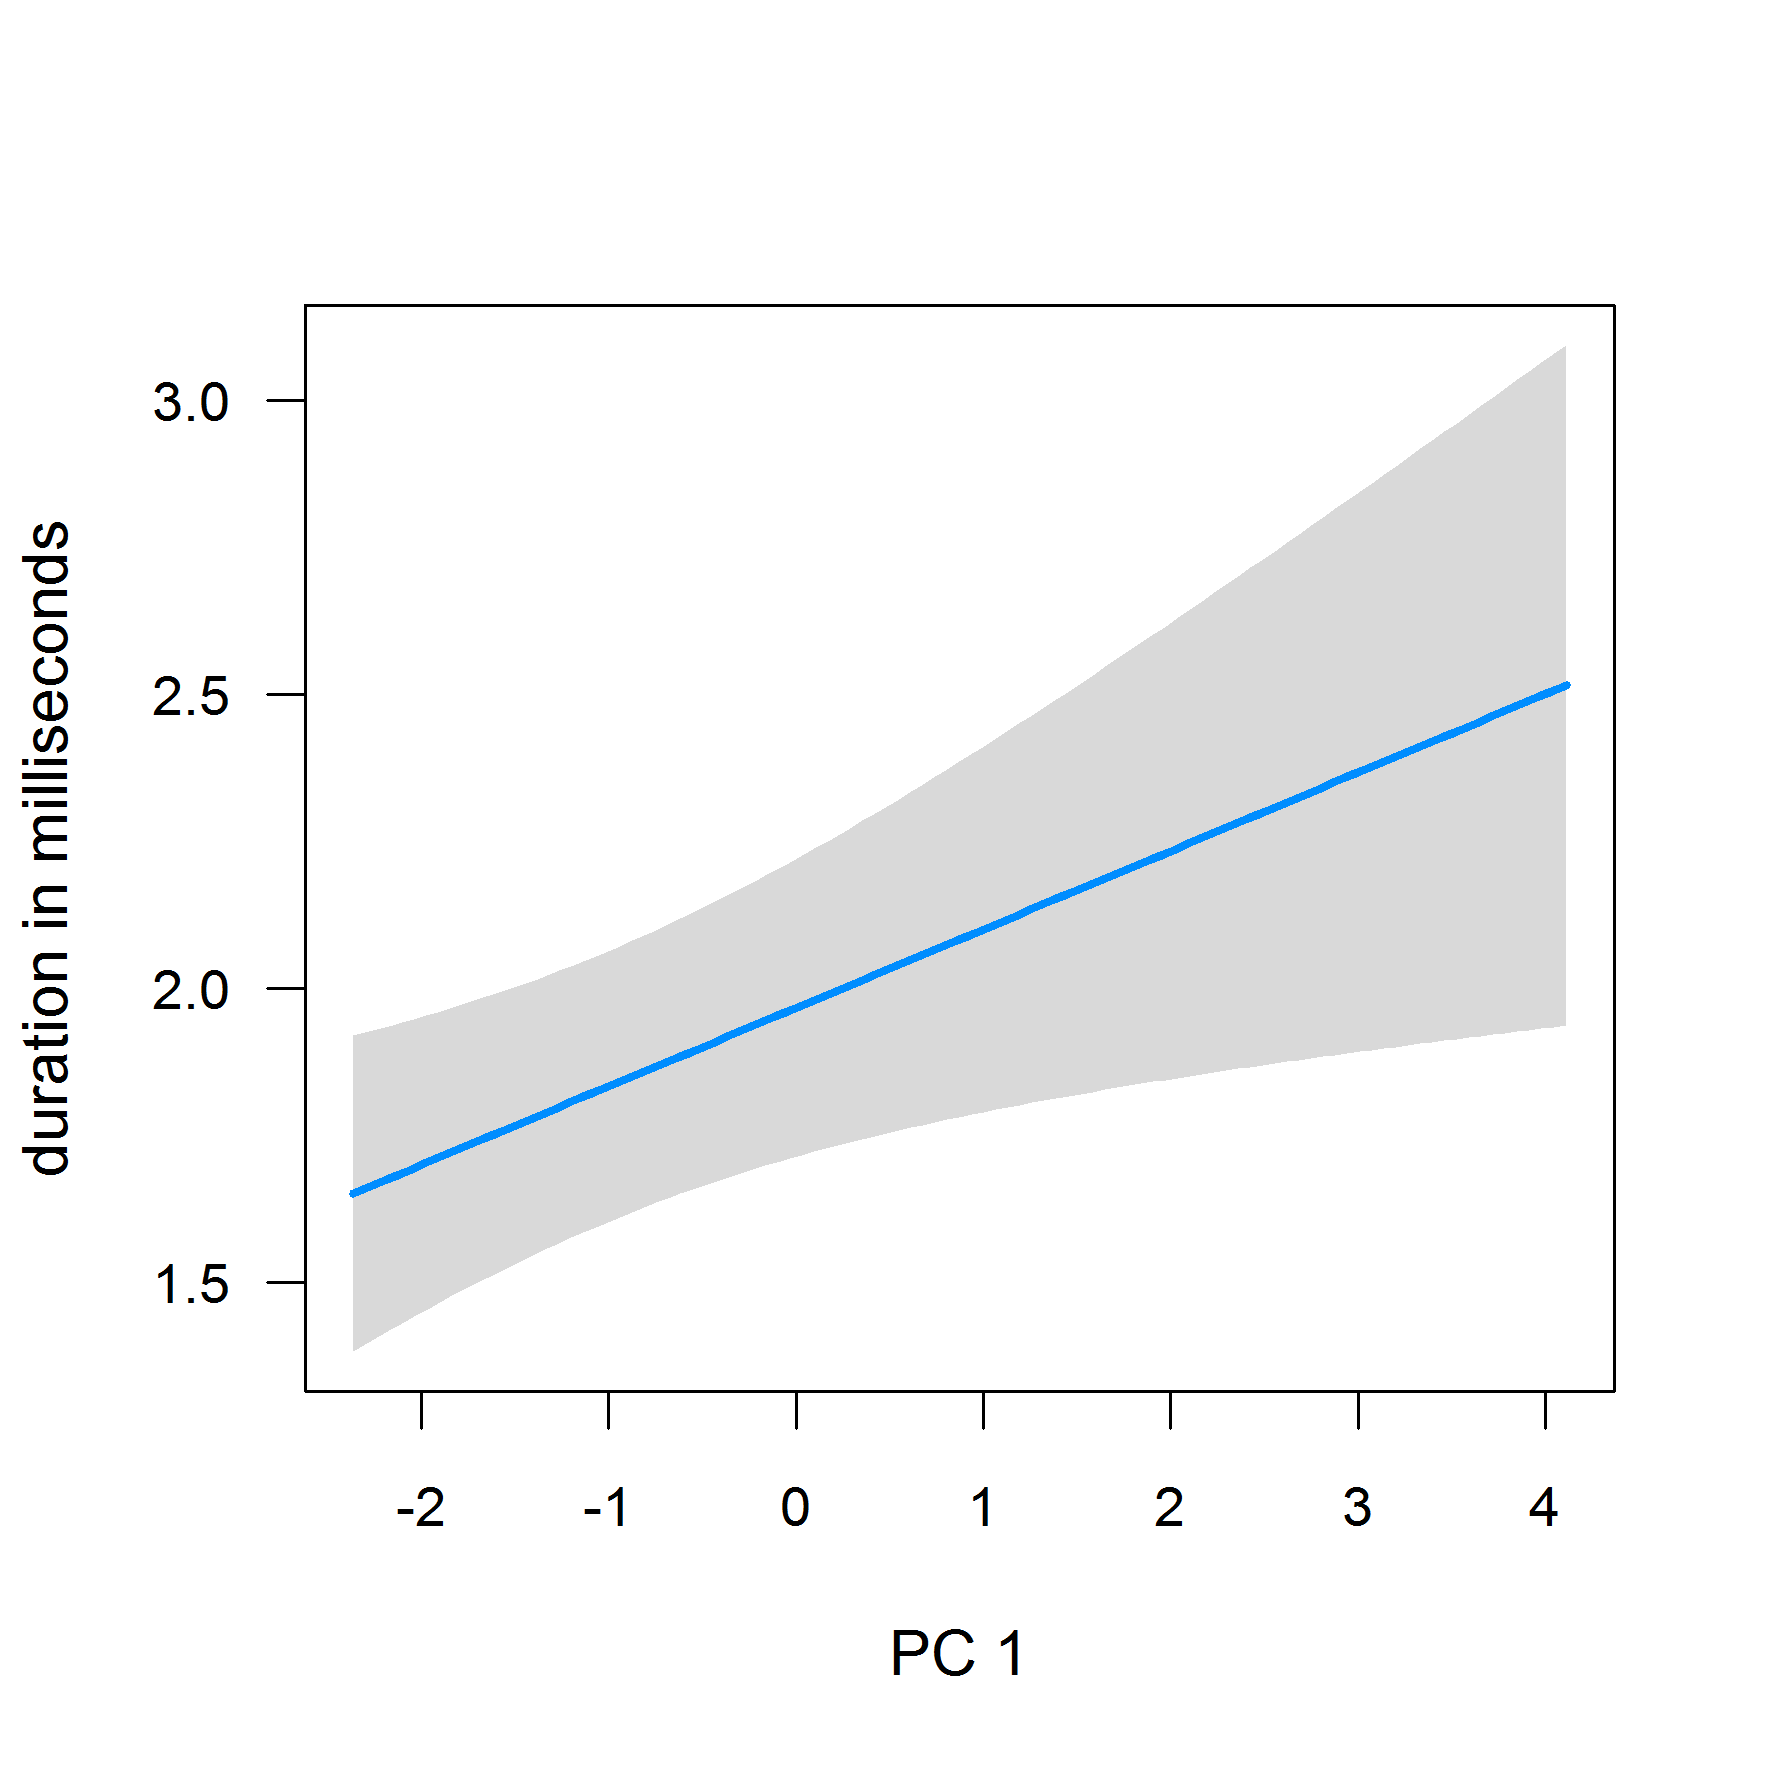
\includegraphics [scale=0.4] {images/Corpus/disPCAbsPC4.png}
	\caption{Effect of PC1 on relative consonant duration in complete \prefix{dis}data set}
	\label{fig:PC1 dis Corpus}
\end{figure*}


The higher the value of \textsc{PC1}, the longer the relative duration of the fricative. As explained above, \textsc{PC1} is composed of all decomposability measures. The higher the \textsc{PC1}-value, the less decomposable a word is.
 One can thus interpret the effect of \textsc{PC1} in the following way: the less decomposable a derivative, the longer the relative duration of /s/. This is unexpected with regard to the decomposability predictions. It is, however, somewhat expected with regard to the results from the complete relative duration model, in which semantically transparent words are predicted to have shorter fricatives than semantically opaque words. As discussed above, this effect might be caused by the distribution of certain properties among types and tokens in the subset, and one must therefore be cautious with the interpretation of the effect. All in all, one can state that the principal component model shows similar effects as the model with the individual decomposability measures, and that the interpretation of the decomposability effect is yet unclear.






As for absolute duration, two multi-model inferencing analyses were conducted to identify the most important variables for predicting relative duration with \prefix{dis}, one for the complete data set and one for the voiceless data set. 
 As in the absolute duration models, \textsc{Environment} is clearly the most important variable in both models (importance value: $1$). In the complete model, \textsc{Voicing} is also of very high importance  (importance value: $0.99$). For both data sets, the first principal component (\textsc{PC1}) reaches a rather high importance value (complete data set: $0.85$,  voiceless data set: $0.71$). The importance values of all other variables are much lower.
\textsc{BaseInitialStress} has an importance value of $0.56$ in the complete data set and one of $0.41$ in the voiceless data set,   
\textsc{PC2} has an importance value of $0.47$ in the complete data set and one of $0.40$ in the voiceless data set,   
\textsc{PC3} has an importance value of $0.27$ in the complete data set and one of $0.28$ in the voiceless data set,   
log\textsc{WordFormFrequency} has an importance value of $0.27$ in the complete data set and one of $0.25$ in the voiceless data set, and  
\textsc{LocalSpeechRate} has an importance value of $0.26$ in the complete data set and one of $0.24$ in the voiceless data set.  

\subsubsection{Summary}


The models predicting absolute duration with \prefix{dis} and the models predicting relative duration with \prefix{dis} reveal similar effects. In general, all models feature the same set of variables, and there are only small differences between the models. The models predicting relative duration feature fewer significant variables, and only in absolute duration models interactions were found to be significant. 
The absolute duration models feature a higher R-squared than the relative duration models. They thus explain more of the variance in the data than the relative duration models. This finding is similar to what was found for \prefix{un} and \prefix{in}. 

%Loc Speech 
With regard to the noise variables, \textsc{LocalSpeechRate}, \textsc{Voicing}  and \textsc{BaseInitialStress} had a significant effect on consonant duration in the models. 
In absolute duration, \textsc{LocalSpeechRate} influenced fricative duration in the expected direction, i.e. the higher the speech rate, the shorter the fricative. \textsc{LocalSpeechRate} did not affect the relative duration of the fricative. 
An effect of \textsc{Voicing} was found in the two models containing all \prefix{dis}prefixed items, i.e. voiced and voiceless items. Voiced items are shorter than voiceless items in absolute and relative duration.
The effect of \textsc{BaseInitialStress} is less clear. While in relative duration, an unstressed base-initial syllable leads to the shortening of the fricative in all \prefix{dis}prefixed words, in the absolute duration models the variable forms interactions. In the model with only voiceless items \textsc{BaseInitialStress} interacts with \textsc{SemanticTransparency},  in the complete model it interacts with \textsc{Environment}.



% The two interactions
Both interactions with the variable \textsc{BaseInitialStress} are caused by only few tokens in the data set, three in the complete model and four in the voiceless model. Three of those tokens are of the type \textit{dissolution}, which is the only type in the data set which is opaque, features a double consonant and has an unstressed base-initial syllable. 
In the voiceless model, we find that in opaque items with an unstressed base-initial syllable, i.e. in the three tokens of the type \textit{dissolution} and in the one token of the type \textit{discount}, consonants are shorter than in all other items. 
In the complete model, we find that doubles in words with an unstressed base-initial syllable, i.e. doubles in the type \textit{dissolution}, are shorter than in all other double consonant items. They are as long as singletons. This means that while all other double consonants geminate, the double consonant in these words is not significantly longer than a singleton.

The two absolute duration models thus predict particularly short fricative durations for the same tokens, in particular tokens of the type \textit{dissolution}. The models differ, however, in how they explain the shortness of the consonant. While in the complete model the short double consonant is explained by the following unstressed syllable, in the voiceless model it is explained by the combination of an unstressed base-initial syllable with semantic opacity. It remains unclear whether the short duration of /s/ in \textit{dissolution} is caused by its unstressed base-initial syllable, i.e. whether all \prefix{dis}prefixed words degeminate when followed by an unstressed syllable, or whether it is caused by the combination of an unstressed base-initial syllable and semantic opacity, or whether this is a type-specific effect.


All in all, the analyses suggest that, in general, \prefix{dis} geminates. Except for the complete absolute duration model, in which one type with a double consonant degeminates, i.e. \textit{dissolution}, all  models show a robust effect of the variable \textsc{Environment}. In both absolute and relative duration, doubles are significantly longer than singletons. There is no significant difference in duration between the two singleton levels. Furthermore, multi-model inferencing supports the claim that \prefix{dis} geminates by showing the importance of the variable \textsc{Environment} for all models. 
One can thus summarize that the corpus study shows that in the majority of cases, the prefix \prefix{dis} geminates. The only \prefix{dis}prefixed word in the data set which might degeminate is the word \textit{dissolution}.

With regard to the other variables of interest, i.e. the decomposability measures, only \textsc{SemanticTransparency} showed a significant effect in absolute duration. The effect was only significant in one model and formed an interaction with \textsc{BaseInitialStress}. As discussed above, the interaction is  caused by only a few items and therefore difficult to interpret.
 In the relative duration models, effects of \textsc{SemanticTranspaency} and \textsc{PC1} were found. Due to the distribution of certain properties in the data set, these effects are, however, also difficult to interpret. 


\subsection{The Suffix \suffix{ly}}


\subsubsection{Absolute duration}

After the exclusion of two outliers, the \suffix{ly}-model showed a satisfactory distribution of residuals, and an initial model was fitted. 
With regard to decomposability, only the two decomposability measures \textsc{LSAScore} and log\textsc{RelativeFrequency} were tested in the model. As described in \sectref{The decomposability of the four affixes: a comparison}, in the \suffix{ly}-data set the variables \textsc{SemanticTransparency}, \textsc{TypeOfBase}  and \textsc{SemanticTransparencyRat-ing} did not show any, or barely any, variation. Therefore, their effect on consonant duration in \suffix{ly} could not be tested. The variable \textsc{PrecedingSegmentDuration} was also discarded. This was because of its high correlation with the variable \textsc{PrecedingSegment}, which would have caused collinearity problems in the model. In preliminary analyses, the variable \textsc{PrecedingSegment} proved to be the better predictor. Therefore, this variable was used in the model and not \textsc{PrecedingSegmentDuration}. 

The model for the \textit{ly-}data set was simplified according to the same procedure as the  previous models. A list of all tested interactions in the model can be found in \hyperref[Appendix C: Summaries of tested interactions in corpus study]{appendix C}. 
The final model is summarized in \tabref {tbl: corpus summary model ly}.


\begin{table*}
	\caption{Summary of linear model for variables predicting the  duration of [l] in \suffix{ly}-suffixed words}
	\label{tbl: corpus summary model ly}
	
					\resizebox{\textwidth}{!}{%		
		
		\begin{tabular}{lrrrr}
			
			
			\lsptoprule
			& Estimate & Std. Error & t-value & p-value  \\ 
			\midrule
			Intercept                           &   77.323& 8.438 & 9.163& $<$0.001\\
			\textsc{Environment}-\texttt{syllabic l\#l} &
			\color{lsLightGray} {7.387}  & \color{lsLightGray} 5.641 &\color{lsLightGray}1.309 &\color{lsLightGray} 0.192 \\
			\textsc{Environment}-\texttt{\#l} &
			\color{lsLightGray} {3.965} & \color{lsLightGray}  4.761 &\color{lsLightGray}0.833  & \color{lsLightGray}0.406 \\
			\textsc{LocalSpeechRate} &                 -2.335 &  0.438 & -5.332& $<$0.001\\
			\textsc{PrecedingSegment} - \texttt{vowel}  &    15.694  &4.429&  3.544  & 0.001\\
				log\textsc{WordFormFrequency} &       -1.631&0.777 &  -2.100 & 0.038 \\		
			\midrule\\
			Adjusted R-squared: 0.236\\
			\lspbottomrule

		\end{tabular}
	}
	
\end{table*}





The model explains about 24\% of the variance and features four variables of which three are significant. The three noise variables \textsc{LocalSpeechRate}, \textsc{PrecedingSegment} and log\textsc{WordFormFrequency} are significant. 
The variable \textsc{Environment} does not show a significant effect but remained in the model as it is the crucial variable with regard to gemination.



\figref{fig:corpus covariates ly} displays the effects of \textsc{LocalSpeechRate} and \textsc{PrecedingSegment}. The left panel of the figure shows that with increasing speech rate /l/ becomes shorter, and the right panel shows that after a vowel /l/ is longer than after a consonant. These effects are expected.





\begin{figure*}
	
		
	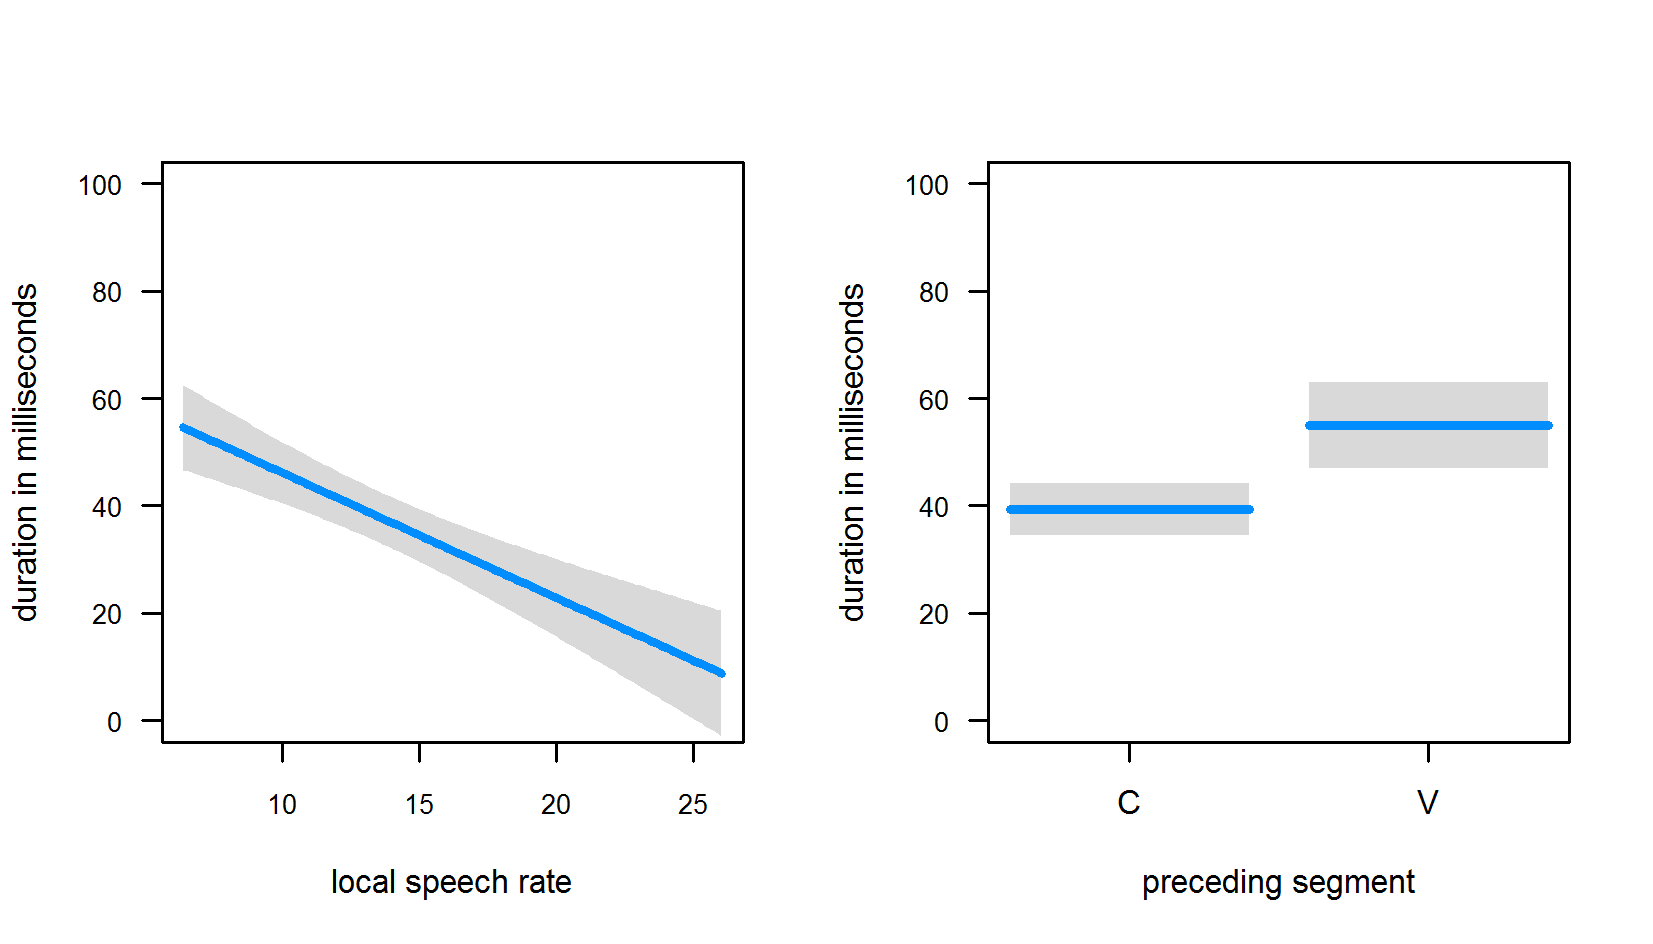
\includegraphics[scale=.8] {images/Corpus/lyModelcov.png}
	\caption{Effects of local speech rate and preceding segment on consonant duration in \suffix{ly}-data set}
	\label{fig:corpus covariates ly}
\end{figure*}





\figref{fig:corpus main effects  ly} shows the effects of log\textsc{WordFormFrequency} and \textsc{Environment}.
The left panel of the figure shows that with increasing frequency /l/ becomes shorter. This is expected.
The right panel of the figure shows the insignificant effect of \textsc{Environment} on consonant duration in \suffix{ly}. The figure clearly shows that there is no durational difference between double /l/ (\texttt{l\#l}), syllabic double /l/ (syllabic \texttt{l\#l}) and singleton /l/ (\texttt{\#l}). The suffix \suffix{ly} thus clearly degeminates in absolute duration. 


\begin{figure*}
	

	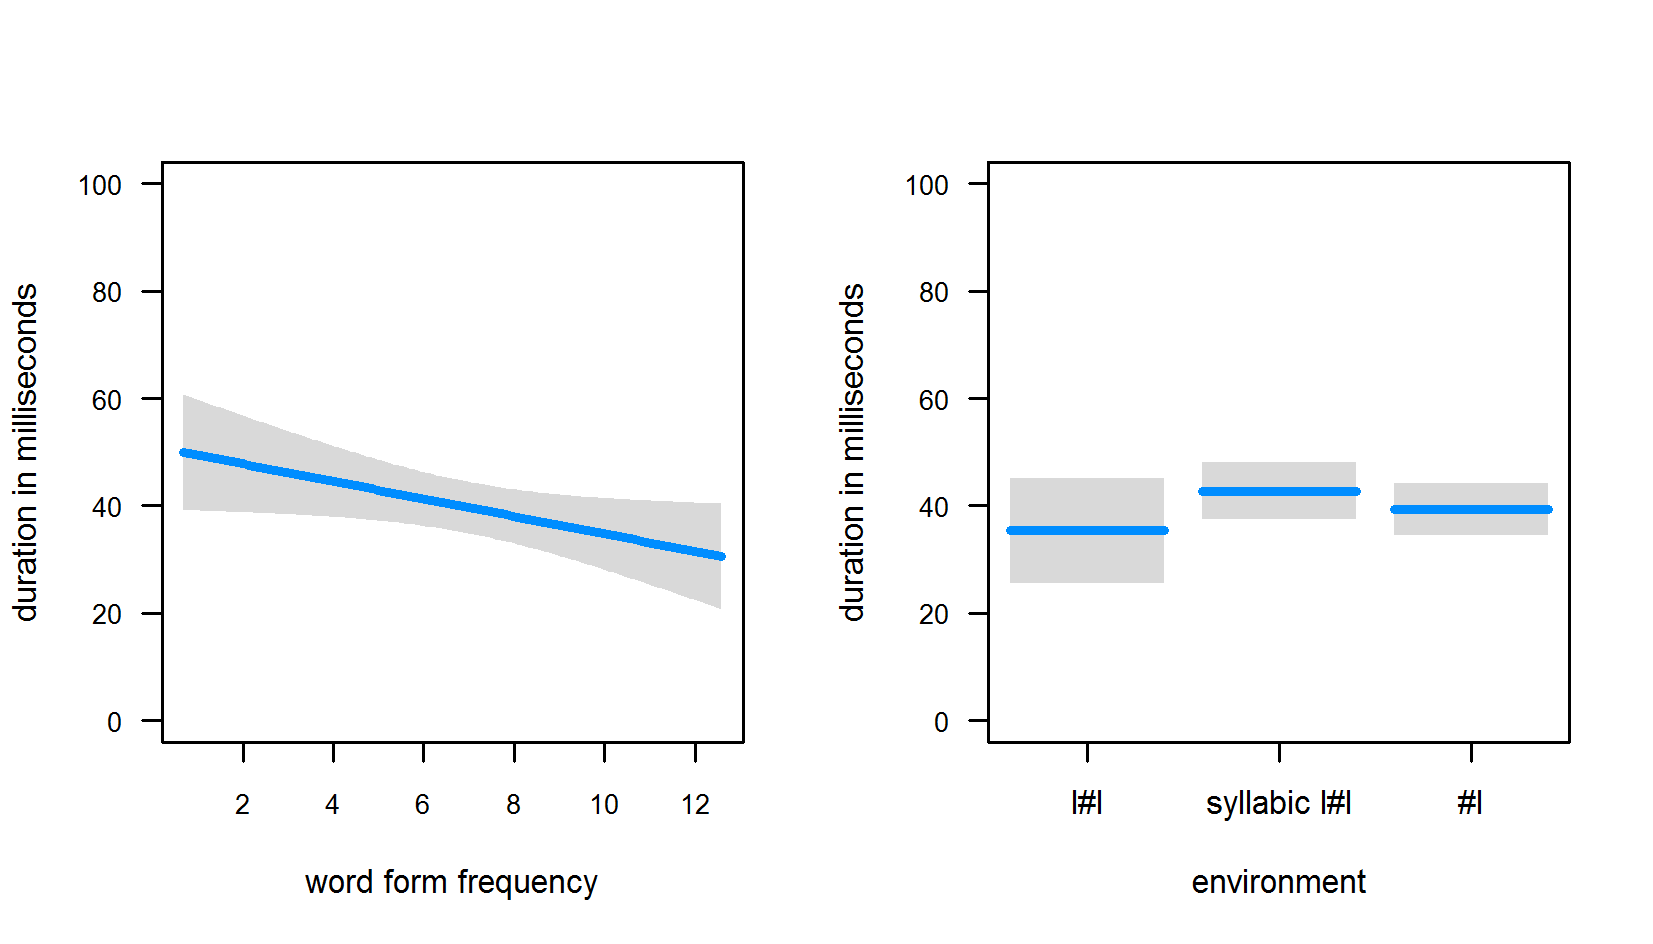
\includegraphics[scale=.8] {images/Corpus/lyModelTransitionTypeAndFreq.png}
	\caption{Effects of word form frequency  and environment on consonant duration in \suffix{ly}-data set}
	\label{fig:corpus main effects  ly}
\end{figure*}




To see which are the most predictive variables for consonant duration in the \suffix{ly}-data set, I conducted a multi-model inferencing analysis. As for the other data sets, the analyses did not include the variable \textsc{LSAScore} because of the low number of observations which were coded for \textsc{LSAScore}. The analysis revealed that \textsc{LocalSpeechRate} is the most important variable (importance value: $1$). With an importance value of $0.99$ the variable \textsc{PrecedingSegment} is the second most important value. It is followed by the two frequency variables log\textsc{RelativeFrequen-cy} (importance value: $0.67$) and log\textsc{WordFormFrequency} (importance value: $0.64$). With importance values of $0.32$ (\textsc{Environment}) and $0.26$ (\textsc{BaseFinalStress}), the other variables are far less important for predicting consonant duration with \suffix{ly}.


\subsubsection{Relative duration}

To test whether the affix \suffix{ly} geminates in terms of relative duration, it was necessary to create a subset. This subset only includes words which feature a vowel at the end of their base, i.e. words in which the suffix is preceded by a vowel. This was necessary because relative duration (as a measure of gemination) is calculated by dividing consonant duration by preceding vowel duration. Since the complete data set includes words which are preceded by a consonant, the creation of the subset was necessary.
However, the subset only includes 48 tokens, i.e. it is very small. Furthermore, in this data set only the difference in duration between two of the pertinent environments can be tested, i.e. \texttt{l\#l} and \texttt{\#l}. The items featuring a syllabic double (\texttt{syllabic l\#l}) had to be excluded since they are always preceded by a consonant. 

The small size of the data set restricted the number of noise variables included in the model, i.e. to avoid overfitting, only few variables were tested in the model. I chose to only include those noise variables which showed a significant effect in the absolute duration model, i.e. \textsc{LocalSpeechRate} and log\textsc{WordFormFrequen-cy}. The variable \textsc{PrecedingSegment} was not included because all of the preceding segments in the data set were vowels. The model was then fitted according to the same procedure as the absolute duration model. The residuals were normally distributed, and thus no transformation of the dependent variable was necessary and no items had to be excluded.

The final model reached an adjusted R-squared of $0.184$, i.e. it explains 18\% of the variance in the data. As with the other affixes, the relative duration model is thus worse than the absolute duration model. Only one variable remained in the final model, log\textsc{WordFormFrequency}. The higher the frequency, the shorter the relative duration of the consonant ($estimate= -0.129$, $t$-$value=-3.533, p=0.001$). In contrast to the absolute duration model, \textsc{LocalSpeechRate} did not reach significance. Crucially, \textsc{Environment} did not reach significance. Doubles are not longer than singletons in terms of relative duration, i.e. they degeminate.
Because of the low number of observations in the subset, no multi-model inferencing analysis was conducted.

\subsubsection{Summary}
Two models predicting consonant duration with \suffix{ly} were fitted, one predicting absolute consonant duration and one predicting relative consonant duration. The usefulness of the relative duration model is, however,  restricted by the small number of observations which were taken into account in this model. In both models only noise variables showed significant effects. 
In the absolute duration model, the expected effects of \textsc{LocalSpeechRate}, \textsc{PrecedingSegment} and log\textsc{WordFormFrequency} were found. In the relative duration model only log\textsc{WordFormFrequency} had a significant effect on consonant duration.
Crucially, the variable \textsc{Environment} did not have a significant effect on consonant duration, neither in absolute nor in relative duration. Multi-model inferencing also showed that this variable is not an important predictor for consonant duration with \suffix{ly}. Thus, the suffix \suffix{ly} clearly degeminates.
The decomposability variables did not prove to be significant in either model.




\subsection{Summary} \label{Summary Corpus Study}

The first durational analyses looked at the distribution of duration across environments to get a first impression of whether the affixes under investigation geminate, and if so, whether gemination is a gradient or a categorical phenomenon. 
For the prefixes, the analyses revealed that the distribution of duration in the data sets is bimodal, with the double consonants being significantly longer than the singletons. This indicates that the prefixes geminate, and that gemination is categorical. The distribution for \suffix{ly} is not bimodal, and doubles are not longer than singletons. This suggests degemination with \suffix{ly}. The impression that the prefixes geminate and that the suffix degeminates was validated in the linear models.


For all data sets at least two linear models were fitted, one predicting absolute consonant duration and one predicting relative consonant duration. 
In general, both models reveal very similar results, i.e. for the most part the same variables are significant in both models. However, the relative models feature fewer variables than the absolute models.  Importantly, the effects of the variables of interest do not differ between the models, i.e. the same variables of interest are significant in both models. The relative duration models only feature less noise variables. 
The variable \textsc{Environment} shows stronger effects in absolute than in relative duration. 
Furthermore, for all affixes, the absolute duration models explain more of the variance in the data than the relative duration models. 
The results thus suggest that absolute consonant duration is a better measure of gemination than relative consonant duration. In other words, gemination in English is not expressed by a particular consonant-vowel ratio but by absolute consonant duration. 
In what follows I will therefore concentrate on absolute consonant duration.

\begin{table*}
	\caption{Overview of significant variables in absolute duration models}
	\label{tbl: Overview of results in the corpus study}
	
	%	
	
		%			\resizebox{\textwidth}{!}{%		
		\begin{tabular} {lccccc}
			
			\lsptoprule
			\textbf{Variable} & \textbf{un-} & \textbf{im-} &\textbf{un-} &\textbf{dis-}& \textbf{-ly}\\
			& & &\& \textbf{im-}  && \\
			\midrule			
			\textsc{Environment}& \checkmark & \checkmark  & \checkmark & \checkmark & n.s. \\ 
			\textsc{Affix }&- &\checkmark  & \checkmark  &- & -\\ 
			
			\textsc{SemanticTransparency}&-& n.s. &  - & (\checkmark) & - \\
			\textsc{LocalSpeechRate}&\checkmark & \checkmark & \checkmark  &\checkmark  & \checkmark \\			
			\textsc{BaseInitialStress}&n.s.& \checkmark & \checkmark & \checkmark &-\\
			\textsc{Voicing}& - & - & - &\checkmark  & - \\
			\textsc{PrecedingSegment}&-& -& - & - &\checkmark\\
			log\textsc{WordFormFrequency}&n.s.& n.s.& n.s. & n.s.&\checkmark\\
			
			\midrule\\
			
			\multicolumn{6}{l}{\small \checkmark \hspace*{0.2cm}: significant in at least one of the absolute duration models} \\			
			\multicolumn{6}{l}{\small n.s. : not significant in any of the absolute duration models} \\			
			\multicolumn{6}{l}{\small - \hspace*{0.45cm}: not included in the absolute duration models} \\	\\
			\lspbottomrule		
			
		\end{tabular}
		%	}
	
	
	
	
\end{table*}


\tabref{tbl: Overview of results in the corpus study} shows an overview of the variables which show significant effects on absolute consonant duration in the subsets. Only variables which are significant in at least one of the absolute duration models are listed. For \prefix{dis}, the table indicates all variables which are significant in at least one of the two absolute duration models fitted, i.e. the model including all \prefix{dis}prefixed items and the model including only voiceless items.







Let us first discuss the noise variables. The variable \textsc{LocalSpeechRate} shows the expected effect in all models.  The higher the speech rate, the shorter the duration of the consonant. 
For \prefix{dis}, the variable \textsc{Voicing} is significant in the complete model. As expected, voiced items are shorter than voiceless items. The variable is irrelevant for all other models.

\textsc{BaseInitialStress} affects consonant duration in the \prefix{in}model and in the \prefix{un} \& \prefix{in} model. Before unstressed base-initial syllables the consonant is shorter than before stressed base-initial syllables. 
In the \prefix{dis}models, \textsc{BaseInitialStress} forms interactions with \textsc{Environment} and \textsc{SemanticTransparency}. As discussed thoroughly in \sectref{corpus results dis}, these interactions were caused by only a few items and their interpretation is therefore unclear. Either only \prefix{dis}prefixed items with a double consonant are affected by \textsc{BaseInitialStress}, or only semantically opaque items are affected by stress.

 \textsc{BaseInitialStress} does not affect consonant duration with \prefix{un}. The reason for the absence of the effect might be due to the distribution of \textsc{BaseInitialStress} across \prefix{un}prefixed words. Most \prefix{un}words feature a stressed base-initial syllable. This includes all items with a double consonant. This lack of variation in stress might have caused the absence of the effect with \prefix{un}. It is also possible that other factors, such as prefixal stress, might have interfered with the effect of \textsc{BaseInitialStress}. As discussed in chapter \ref{affixes}, the stress status of \prefix{un} is yet unclear. Further research on prefixal stress is necessary to explore the relation of stress and prefixal consonant duration further. This is, however, beyond the scope of this study.

For the suffix \suffix{ly}, the two variables \textsc{PrecedingSegment} and log\textsc{WordFormFre-quency} show the expected effects. The consonant is shorter after a consonant than after a vowel, and more frequent words display shorter consonant durations than less frequent words. While \textsc{PrecedingSegment} was only coded for \suffix{ly}, the variable log\textsc{WordFormFrequency} was included in all models. Only for \suffix{ly} it affected consonant duration. There are various possible explanations for this. 
One possibility is that word form frequency only affects consonant duration in suffixes but not in prefixes. Another possibility is that, while the effect exists for all affixes, it only reaches significance in the \suffix{ly}-model. There are two arguments for this explanation.
 First, the \suffix{ly}-model is the worst of all models, i.e. it explains the least variance. It is therefore easier for weaker effects to reach significance. 
 Second, out of all data sets the \suffix{ly}-data set features the highest number of different types. Different types have different frequencies, i.e. the distribution of log\textsc{WordFormFrequency} shows more variation in the \suffix{ly}-data set than in the other data sets. As already discussed above, the lack of variation in the distribution of a variable might make it impossible to find effects. In other words, there might not be enough variation in log\textsc{WordFormFrequency} in the prefixal data sets to find effects.


Let us now turn to the variables of interest. Out of the five decomposability measures only \textsc{SemanticTransparency} showed an effect on consonant duration. This effect was, however, only found in one model, i.e. the model predicting absolute consonant duration with voiceless \prefix{dis}.  Furthermore, the effect was only found in interaction with the variable \textsc{BaseInitialStress}. Since the interaction was caused by only a few items in the data set, its validity is yet unclear. 
In none of the other models decomposability directly played a role. 
However, in two of the models decomposability indirectly influenced duration. As discussed in \sectref{corpus dec}, the five affixes differ in their overall segmentability. This difference is mirrored in consonant duration in the \prefix{in} and in the \prefix{un} and \prefix{in} model. In these models, the variable \textsc{Affix} significantly affects consonant duration. The affix \prefix{un} features the longest nasal, negative \prefix{in} features a significantly shorter nasal, and locative \prefix{in} has the shortest nasal out of the three. This decline in duration resembles the decline in segmentability of the affixes. The prefix \prefix{un} is the most segmentable affix of the three, followed by negative \prefix{in}, followed by locative \prefix{in}. Thus, while word-specific decomposability measures did not affect consonant duration in the models, decomposability influenced consonant duration in terms of the overall segmentability of the affix.


The variable \textsc{Environment} significantly affected consonant duration in all prefixal models. For \suffix{ly}, there was no significant difference in duration between the three tested environments.
\tabref{tbl: Overview of environment in the corpus study} summarizes the predicted durations for all environments for all affixes. The table also shows the significant differences in predicted durations between doubles and singletons for the prefixes, as well as singleton-geminate ratios.
The conditions of the predicted values are the same as in the partial effects plots, i.e. numerical variables are held constant at their median and categorical variables are held constant at the most common category. For \prefix{dis}, two predicted values are shown, one for the complete data set (for words with a stressed base-initial syllable), and one for the voiceless data set.







\begin{table}
	\caption{Overview of predicted durations in the corpus studies}
	\label{tbl: Overview of environment in the corpus study}
	
	
					\resizebox{\textwidth}{!}{%		
		\begin{tabular} {lcccc}
		\lsptoprule
			
			\multicolumn{5}{l}{\textbf{Predicted durations}}\\
					\\
			&  \multicolumn{2}{c}{Phonological Doubles } &  \multicolumn{2}{c}{Phonological Singletons } \\
		%	&in Complex Words & in Complex Words &in Complex Words\\
			& 					(non-syllabic)						&(syllabic)			& (consonant-adjacent) &(vowel-adjacent)\\
			%	&Double -Singleton & Double -Singleton &\\
			\midrule			
			un-& 90~ms &NA& 63~ms   & 43~ms\\ 
			im-& 95~ms&NA& 68~ms & NA  \\ 

			dis-\textsuperscript{1}   & 136~ms&NA& 98~ms& 113~ms\\
			dis-\textsuperscript{2}&142~ms&NA& 98~ms &  97~ms\\

			%& Phonological Doubles & Phonological Doubles &Phonological Singleton \\
				%		&in Complex Words & in Complex Words &in Complex Words\\
			%&(non-syllabic)&(syllabic) &\\

			-ly&35~ms& 43~ms &   \multicolumn{2}{c}{39~ms}\\
			
			
			\midrule

			\\
			
						\\
						\multicolumn{3}{l}{\textbf{Durational difference}}&\multicolumn{2}{l}{\textbf{Singleton-Geminate Ratio}}\\
						\\			
						&Double-Singleton  &Double-Singleton  &Singleton-Double  &Singleton-Double  \\
						&(consonant-adjacent) &(vowel-adjacent)& (consonant-adjacent) &(vowel-adjacent)\\


			%	&Double -Singleton & Double -Singleton &\\
			\midrule			
			un-& 27~ms & 47~ms   & 1:1.4 & 1:2.1\\ 
			im-&27~ms &NA  & 1:1.4 & NA\\ 
			dis-\textsuperscript{1}  &38~ms& 23~ms & 1:1.4& 1:1.2 \\
			dis-\textsuperscript{2} &44~ms& 45~ms &1:1.5& 1:1.5\\
			
			%-ly&- & - & &  \\			
			
			\midrule
			\\

			\multicolumn{5}{l}{\textsuperscript{1} \footnotesize{stressed base-initial syllable}}\\
			\multicolumn{5}{l}{\textsuperscript{2} \footnotesize{voiceless}}\\
			\lspbottomrule

		\end{tabular}
	}
	
	

	
\end{table}


For \prefix{un}, \prefix{in} and \prefix{dis}, double consonants are significantly longer than corresponding singletons. The only exception might be the double consonant in the word \textit{dissolution}. In the \prefix{dis}model with all words, i.e. voiced and voiceless \prefix{dis}pre-fixed words, a significant interaction between \textsc{Environment} and \textsc{BaseInitialStress} was found. Double consonant items with an unstressed base-initial syllable, i.e. words of the type \textit{dissolution}, degeminated. However, it is yet unclear whether this effect is universal, i.e. whether it applies to all \prefix{dis}prefixed words with a double consonant and an unstressed base-initial syllable,  or whether the effect is caused by other factors, such as the word's opacity or type-specific effects. In chapter \ref{Experimental Studies}, we will turn back to this question after considering the results of the experimental study.

The durational differences between doubles and singletons range from 23~ms to 47~ms.  The singleton-double ratio for singletons followed by a consonant is comparable across all prefixes. The ratio is 1:1.4 for \prefix{un}, \prefix{in}, and \prefix{dis} (in the complete data set). For voiceless \prefix{dis} the ratio is 1:1.5.
For singletons followed by a vowel, the absolute durational difference between doubles and singletons is practically the same for \prefix{un} and voiceless \prefix{dis} (47~ms and 45~ms), but smaller for voiced and voiceless \prefix{dis} (23~ms). The absolute durational differences for \prefix{dis} and \prefix{un} suggest that both prefixes geminate to the same degree. However, the double-singleton ratios suggest the opposite. The ratio for \prefix{un} is much bigger than the ones for \prefix{dis}. This indicates that \prefix{un} geminates to a higher degree than \prefix{dis}


In addition to the difference between doubles and singletons, a significant difference between the two singleton levels was found for \prefix{un}. Consonants followed by a vowel are significantly shorter than consonants followed by a consonant. This difference between the two singleton environments was not found for \prefix{dis}. For \suffix{ly} the variable \textsc{Environment} never reached significance, i.e. singletons, non-syllabic doubles and syllabic doubles are predicted to be of the same duration.

 A comparison of the singleton-double ratios found in this study with the ones in former studies is limited. Only two studies have investigated gemination with the investigated affixes, i.e. \cite{Kaye.2005} and \cite{Oh.2012}. Out of the two, only \cite{Oh.2012} provide enough data for a sensible comparison. The comparison with \citeauthor{Oh.2012}'s study is, however, also restricted as they only investigated the prefixes \prefix{un} and \prefix{in} under experimental condition. Furthermore, consonant duration was only analyzed in intervocalic position, which forbids a straightforward comparison. 
 
 For \prefix{un}, \cite{Oh.2012} find a ratio of 1:1.6 in normal speech, and a ratio of 1:2.0 in careful speech. For \prefix{in}, they find a ratio of 1:1.3 in normal and a ratio of 1:1.2 in careful speech. 
 As normal speech can be assumed to be more similar to conversational speech than careful speech, the singleton-geminate ratios of the present corpus study should be compared to the ones for normal speech. 
 For both \prefix{un} and \prefix{in}, the comparison shows that the ratios found in the present study are bigger than the ones in \cite{Oh.2012}. 
  One reason for this difference might be the different conditions under which the items were recorded, i.e. natural conversation vs. experimental reading. The experimental study on gemination will shed more light on this issue.

To summarize, the prefixes \prefix{un}, \prefix{in} and \prefix{dis} geminate. The suffix \suffix{ly} degeminates. No word-specific effect of decomposability was found, but the segmentability of the affix affected consonant duration in the expected way. Less segmentable affixes have shorter consonant durations. The effect of affix is independent of gemination, i.e. all prefixes geminate. The comparison of singleton-geminate ratios indicates, however, that the prefix \prefix{un} geminates to a higher degree than the prefix \prefix{dis}.

\subsection{Discussion}


The corpus study shows that gemination is affix-specific and categorical. While the prefixes geminate, the suffix \suffix{ly} degeminates. 
This result falsifies common assumptions about the gemination pattern of English affixes as found in the literature (cf. \sectref{assumption gem English}). 
With regard to the theoretical approaches discussed in chapter \ref{Theory}, the result falsifies word-specific approaches, and supports approaches which predict categorical gemination that depends on the affix. However, as thoroughly discussed in chapter \ref{Theory}, there are important differences in the predictions of the affix-specific approaches. In other words, the affix-specific approaches make different predictions about which affixes should geminate and which should degeminate. Therefore, it is necessary to look at the predictions of each of these approaches individually, and to compare them to the gemination pattern found in the study.

Let us first look at the formal linguistic approaches discussed. Even though all of them are categorical in nature and predict gemination to be affix-specific, none of them is supported by the data. The fact that the level 2 affix \suffix{ly} degeminates, while the level 1 affixes \prefix{dis} and \prefix{in} geminate, falsifies the predictions made by stratal approaches. That \prefix{in} and \prefix{dis} geminate furthermore falsifies the predictions made by the Prosodic Word Approach according to which one should find variation in their gemination pattern. 

With regard to the psycholinguistic approaches discussed, only the two affix-specific approaches can be supported by data, i.e. the affix-specific Segmentability Approach and the affix-specific Morphological Informativeness Approach. 
These two approaches are based on the two lexical segmentability hierarchies introduced in chapter \ref{affixes} (see \figref{fig:Segmentability hierarchies of  affixes repetition 2} for the two hierarchies). While the affix-specific Morphological Informativeness Approach predicts gemination to pattern according to the Semantic Segmentability Hierarchy, the affix-specific Segmentability Approach does not specify according to which of the two segmentability hierarchies gemination should pattern. In other words, while the affix-specific Morphological Informativeness Approach is only supported if gemination patterns according to the Semantic Segmentability Hierarchy, the affix-specific Segmentability Approach is also supported if gemination patterns according to the Non-Semantic Segmentability Hierarchy. 


The corpus study reveals that gemination, at least partly, patterns according to the Semantic Segmentability Hierarchy (\prefix{un} > \{\prefix{dis}, \prefix{in}\textsubscript{\textsc{Neg}}\} >  \prefix{in}\textsubscript{\textsc{Loc}} > \suffix{ly}). % according to which  \prefix{un} is the most segmentable and most informative affix, followed by negative \prefix{in} and \prefix{dis}, followed by locative \prefix{in}, followed by \suffix{ly}. 
The least segmentable and least informative affix \suffix{ly} degeminates, while all other affixes geminate. The most segmentable affix \prefix{un} displays a higher singleton-geminate ratio than the less segmentable affix \prefix{dis}, i.e. \prefix{un} geminates to a higher degree than \prefix{dis}. However, the data does not suggest a difference in degree of gemination between \prefix{in} and \prefix{un}, or between the two \prefix{in}prefixes.
 It is not yet clear whether such differences are non-existent, or whether, due to methodological reasons, they were not detected in the data set. 
  In contrast to \prefix{un} and \prefix{dis}, only two environments were investigated for \prefix{in}, i.e. \texttt{m\#mV} and \texttt{m\#C}. The difference in degree of gemination between \prefix{un} and \prefix{dis} was only detected by comparing the singleton-geminate ratio of doubles and singletons followed by a vowel, a ratio which could not be calculated for \prefix{in}. Thus, there might be differences between the degree of gemination of \prefix{un} and \prefix{in} which could not be detected in this study.
Furthermore, the model directly comparing \prefix{un}, negative \prefix{in} and locative \prefix{in} indicates that the difference in segmentability and informativeness between the three prefixes affects their phonetic realization in the predicted direction. The model revealed that the nasal in \prefix{un} is longer than the one in negative \prefix{in}, which in turn is longer than the one in locative \prefix{in}. Thus, while there is no difference in the degree of gemination between the three prefixes, there is a general difference in  their nasal duration.
 
 To conclude, the corpus study provides evidence that the phonetic realization of the investigated affixes, including the realization of morphological geminates, patterns according to the Semantic Segmentability Hierarchy. The pattern of gemination is, however, not yet clear and further evidence is needed. 
 Up until now, the affix-specific Segmentability Approach (which is based on the Semantic Segmentability Hierarchy) and the affix-specific Morphological Informativeness Approach are the only two approaches not falsified by the data, i.e. they are the two approaches which, based on the corpus study, explain gemination in English affixation the best.


Apart from evidence for the gemination pattern of English affixes, the corpus study also revealed important insights with regard to the phonetic realization of alleged homophones. The data shows that there is a durational difference between the two \prefix{in}prefixes. This has important implications for current models of speech production. Models which do not allow for morphological information to be visible on the phonetic level need to be revised with regard to this aspect.



While the corpus study has revealed some important insights for theories of the morpho-phonological interface, a number of questions remain  unanswered. Due to the limited number of types and tokens, some effects could not be investigated properly in the study, i.e the distribution of the data did not allow for valid investigations of some factors. Furthermore, one must complement the corpus data by experimental data, which is more controlled and therefore less prone to distorting effects.
